\chapter{Track reconstruction performance}
\label{chap:tracking-performance}
Track reconstruction identifies a track candidate as the digital realization of a particle trajectory. 
In the GNN-based chain, after graph segmentation, a track candidate is a list of 3-dimensional estimates of the intersections between a trajectory and different detector layers. 
The analysis of tracking performance starts with the extraction of track parameters by a $\chi^2$-fit over on the measurements contained in the candidate.
These parameters characterize the impact parameters and the momentum of the particle, which are crucial information for downstream tasks in event reconstruction. 
We have described the principles of track fitting in section \ref{sect:track-fit}.
The parameter extraction in this chapter closely follows this description, with a small number of adaptations described in section \ref{sect:chi2-fit}.

To evaluate the tracking efficiency, fake rate, and parameter resolution, fitted tracks are matched to generator-level truth particles, which must satisfy a number of criteria on reconstructibility and kinematics.
Section \ref{sect:track-match-metrics} describes the matching procedure and the metrics under which the performance is assessed.

Finally, section \ref{sect:track-performance} is an apple-to-apple comparison between GNN4ITk and CKF tracking performance.


% Different from a track candidate produced by the CKF, by itself does not provide any useful physical information about the trajectory. 
%  Only by fitting a track model through these measurements can we extract a set of track parameters that describe the momentum and impact parameters of the particle. This chapter describes elements of track fitting using the Least-Square Method and the Kalman Filter in ATLAS, laying the foundation for the discussion in subsequent chapters.

\section{Extraction of track parameters}
\label{sect:chi2-fit}

% The least-square method for parameter estimation is ubiquitously used to extract unknown quantities from data. 
As mentioned in section \ref{sect:track-fit}, the tracking model used in ATLAS considers the local coordinates of individual clusters as measurements.
A GNN track candidate, however, is a list of space points reconstructed from these clusters, according to section \ref{sect:cluster-spacepoint}. 
To carry out the fit, the space points are first matched to their corresponding clusters. 
A pixel space point is matched to a unique pixel cluster, while a strip space point is matched to two strip clusters, each from one side of a barrel stave or an endcap petal (see section \ref{sect:itk-overview}). 
The building block of track candidates is a major difference between the GNN-based and the current tracking algorithm, which has implications in the interpretation of results.

To fully characterize a charged particle's trajectory in a magnetic field, the parametrization must specify its global position, momentum and charge at any given point. 
Various conventions satisfy this requirement. 
In the offline analysis framework of ATLAS, the following track parametrization convention is chosen as part of the Event Data Model (EDM) \cite{ATL-SOFT-PUB-2006-004}
\beq
\label{eq:tracking-performance:1}
\mathbf{x} = (
    l^{(1)} , l^{(2)} , \phi , \theta , q/p 
)^T
\eeq
where $(l^{(1)}, l^{(2)})$ denote the coordinates of the intersection between the measuring surface and the trajectory in the local frame of reference, $\phi \in [-\pi, \pi]$ and $\theta \in [0, \pi]$ respectively the azimuthal angle and the polar angle in the global frame of the current location, and $q/p$ the inverse momentum signed by the particle charge. 
The track parameters vary continuously along the trajectory, and the measurements are ``snapshots" taken at the active layers that it traverses. 
The local coordinates $(l^{(1)}, l^{(2)})$ take different meaning depending on the measuring surface. 
For example, on a disk, they are the polar coordinates $(l^{(1)}, l^{(2)}) = (R_{loc}, \phi_{loc})$ of the cluster, while on a plane, they are given in Cartesian coordinates $(l^{(1)}, l^{(2)}) = (X_{loc}, Y_{loc})$.
The perigee parametrization, shown in figure \ref{fig:track-param}, is an imaginary cylindrical surface parallel to the global $z$-axis and passing through the point of closest approach to the origin\footnote{This point is defined as the perigee, hence the designation.}.
The local parameters $(l^{(1)}, l^{(2)}) = (d_0, z_0)$ are respectively the transverse and longitudinal impact parameters, which, along with other global parameters estimated at this position, are reported as \textit{the} track parameters of the corresponding hypothetical particle. 
The perigee parameters are the quantity denoted by $\mathbf{x}_0$ in the discussion in \ref{sect:track-fit}.

\begin{figure}[h!]
    \centering
    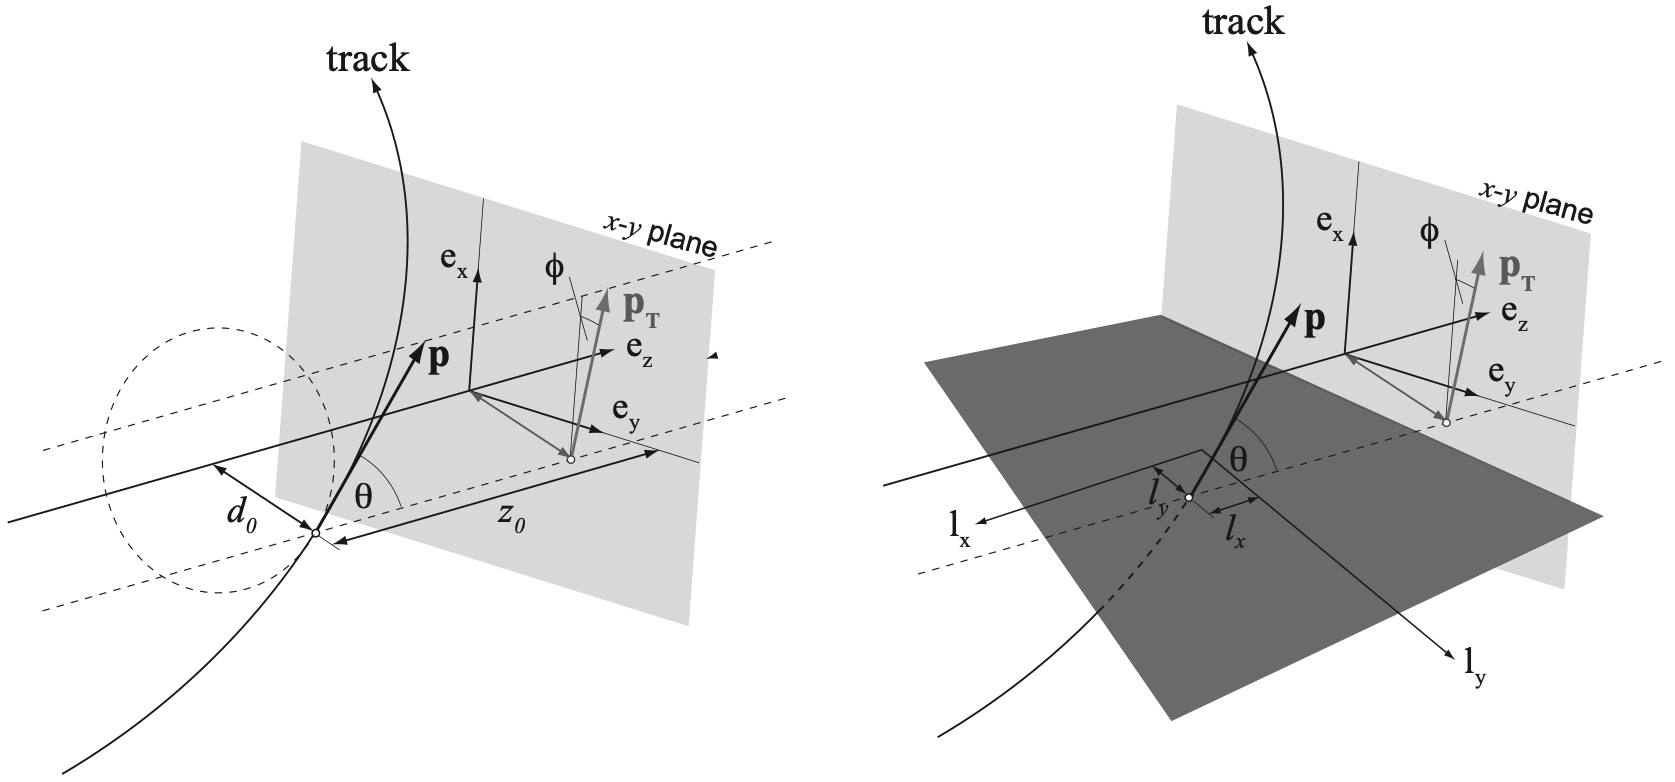
\includegraphics[width=\textwidth]{figures/track-param.png}
    \caption{A track represented in two different parametrizations, both being particular instances of the general ATLAS parametrization in equation \eqref{eq:tracking-performance:1}. The perigee parametrization (left) is defined with respect to the global $z$-axis, while the planar parametrization (right) is defined with respect to the coordinate axes of a local measuring surface \cite{ATL-SOFT-PUB-2007-003}.}
    \label{fig:track-param}
\end{figure}

Thanks to this parametrization, the measurement model is a simple identity projection of the first two track parameter parameters. 
The $i$-th measurement on track is given by
\beq
\label{eq:track-performance:2}
\mathbf{m}_i = \mathbf{H}_i \mathbf{x}_i = \begin{bmatrix} 
    1 & 0 & 0 & 0 & 0 \\
    0 & 1 & 0 & 0 & 0
\end{bmatrix} 
\begin{bmatrix}
    l^{(1)} \\ l^{(2)} \\ \phi \\ \theta \\ q/p 
\end{bmatrix} = 
\begin{bmatrix}
    l^{(1)} \\ l^{(2)}
\end{bmatrix}.
\eeq
The measurement uncertainty is codified in the covariance matrix 
\beq
\label{eq:track-performance:3}
[\mathbf{V}_i]_{jk} = \begin{cases}
    \sigma^2(l^{(j)}_i), \quad & i=j \\
    \rho(l^{(j)}_i, l^{(k)}_i), \quad & j\ne k
\end{cases}
\eeq
which is a block of the covariance matrix of the track parameters
\beq
\label{eq:track-performance:4}
[\mathbf{C}_i]_{jk} = \begin{cases}
    \sigma^2(\mathbf{x}_i^{(j)}), \quad & j=k \\
    \rho(\mathbf{x}_i^{(j)}, \mathbf{x}_i^{(k)}), \quad & j\ne k
\end{cases}
\eeq
where $\mathbf{x}^{(i)}$ is the $i$-th component of the track parameters, $\sigma^2(X)$ the variance of $X$ and $\rho(X,Y)$ the covariance of $X$ and $Y$. 

% A DISCUSSION ON TRACK PROPAGATION. THIS COULD BE MOVED TO THE CKF CHAPTER, BUT NECESSARY TO ADD A REMINDER HERE AND EMPHASIZE THE HOW MATERIAL EFFECTS ARE MODELLED.
Given the track state $\bfx$ and a covariance $\mathbf{C}$ at any point on the trajectory, an estimate of the state at a another point $\bfx'$ can be obtained by numerically integrating the EOM, as described
in section \ref{sect:chi2-fit}. 
If the position of $\bfx'$ coincides with a sensitive element, an expected value of the corresponding measurement could be derived using equation \eqref{eq:track-performance:2}, allowing to write 
the measurement error as a function of $\bfx$.
Repeating this process, taking $\bfx$ as the initial value, we can define the measurement error of the entire track candidate and optimize for $\bfx$.

Let $M=\{\mathbf{m}_1, \dotsc , \mathbf{m}_N\}$ be the set of all clusters matched to the track candidate. The cost function can be written as a function of an initial state $\mathbf{x}$ as
\beq
\label{eq:track-performance:5}
\boxed{\mathcal{L}_{M}(\mathbf{x}, \vartheta) = \frac{1}{2}\sum_{i=1}^{N} [\mathbf{m}_i - \mathbf{H}_i f_i(\mathbf{x}, \vartheta) ]^T \mathbf{V}_i^{-1} [\mathbf{m}_i - \mathbf{H}_i f_i(\mathbf{x}, \vartheta) ] + \frac{1}{2}\sum_{j=1}^{J} \frac{\vartheta_j^2}{\sigma^2(\vartheta_j)},}
\eeq
in which, as discussed in section \ref{sect:track-fit}, the set of angles $\{\vartheta_j\}$  is included to model small-angle multiple scatterings due to interaction with the detector material. 
These angles are assumed to be normally distributed with mean $\expval{\vartheta_j}=0$ and variance estimated by the Highland formula \eqref{eq:6.14}. 
It is important to note that these scattering angles are floated as fit parameters, but they are constrained by the variances $\sigma^2(\vartheta_j)$ which \textbf{are} functions of the trajectory and therefore the initial state $\mathbf{x}$.

Since the cost function is no longer linear, an analytical solution to the equation 
\beq
\label{eq:track-performance:4-1}
\nabla\mathcal{L}_M (\mathbf{x}, {\vartheta}) = 0
\eeq
does not exist.
Instead, it must be numerically minimized, starting from some initial value $\tilde{\mathbf{x}}$.
To estimate $\tilde{\mathbf{x}}$, a circle fit using the conformal map method is performed over the $(x,y)$ coordinates the first three space points of the track candidate. 
This procedure is described in reference \cite{HANSROUL1988498}. 
The crude estimate is fed into the optimizer, along with the cost function to obtain a globally optimal estimate $\hat{\mathbf{x}}$ of the track parameters. 
\beq
\label{eq:track-performance:6}
\hat{\mathbf{x }} = \min_{\mathbf{x}} \mathcal{L}_M(\mathbf{x}, \vartheta)
\eeq

% A discussion on outliers and outlier removal

\section{Track matching and performance metrics}
\label{sect:track-match-metrics}

In simple terms, tracking performance is evaluated by answering the following questions
\begin{enumerate}
    \item \textbf{Efficiency}: How many \textit{relevant} truth particles are reconstructed?
    \item \textbf{Fake rate}: How many tracks are created but represent no truth particles?
    \item \textbf{Track quality}: How well does a reconstructed track represent the corresponding truth particle?
\end{enumerate}
Since all three items compare tracks to particles, it is necessary to match the reconstructed track candidates and truth-level particles. 
It is for this reason that the evaluation can only be done with Monte-Carlo simulation where truth information is available. 

\begin{definition}
    \label{def:tracking-efficiency}
    The tracking efficiency $(\epsilon_{track})$ is the fraction of prompt particles associated with track candidates passing some quality selection. 
    \beq \label{eq:track-performance:7}
    \epsilon_{track} = \frac{N_{reco}}{N_{truth}},
    \eeq
    in which $N_{truth}$ is the number of particle passing a set of reconstructibility criteria, and $N_{reco}$ the number of those matched to a ``good" track candidate.
\end{definition}
It is important to distinguish the tracking efficiency the edge efficiency defined in equation \eqref{eq:9.2}. 
The former is defined on the set of truth particles, while the latter the set of edges between space points reconstructed from truth particles. 
While the edge efficiency is useful in machine learning development, only the tracking efficiency is meaningful in the performance presented in this chapter, and, to a larger extent, in the ATLAS event reconstruction chain.

A matched track candidate is required to have a high matching probability with the particle in question, defined as follows.
\begin{definition}
    \label{def:matching-prob}
    Matching probability $P_m{(A,B)}$: Let $A$ denote both a track candidate and the set of clusters it contains, and $B$ those of a particle. The matching probability between track $A$ and particle $B$ is the weighted fraction of clusters contained in $A$ that are in common with $B$.
    \beq \label{eq:track-performance:8}
        P_m{(A,B)} = \frac{2\abs{(A\cap B)_{pix}} + \abs{(A\cap B)_{strip}} }{  2\abs{A_{pix}} + \abs{A_{strip}  } },
    \eeq
    where $S_{pix}$ and $S_{strip}$ respectively denote the subsets of pixel and strip clusters of set $S$.
\end{definition}
Intuitively, a track candidate has a high probability of matching to a particle if the majority of its hits originate from that particle. 
The factor of 2 gives a doublet the weight to a pixel cluster, because it provides a 2D measurement of the track, whereas a strip cluster provides only 1\footnote{Remember that it takes 2 measurements (2 clusters) from a double-sided strip layer to form a 3D space point.}.
A track $A$ is said to be matched to a particle $B$ if its matching probability $$P_m(A,B) > 0.5.$$
Tracks candidates that are not matched to any particle are said to be fake.
The fake rate is thus defined as follows.
\begin{definition}
    \label{def:fake-rate}
    The fake rate $F_{track}$ is the fraction of reconstructed track candidates having the highest matching probability not exceeding 0.5
    \beq \label{eq:track-performance:9}
        F_{track} = \frac{1}{N_{track}} \sum_{i=1}^{N_{track}} \mathbb{I}_{[\max_j P_m(A_i, B_j) \le 0.5 ]} = \frac{N_{fake}}{N_{track}},
    \eeq
    where $\mathbb{I}$ is the indicator function.  
\end{definition}
Definitions \ref{def:tracking-efficiency} and \ref{def:fake-rate} thus answer questions (1) and (2).

The track quality is a comparison between the properties of truth particles, including momentum, cluster composition, and impact parameters, to those of the matched track candidate. 
The track properties are estimated by the track fit described in \ref{sect:chi2-fit}. 
Most important among them are the track parameter resolution, defined as
\begin{equation}
\label{eq:track-performance:11}
    \sigma(\mathbf{x}^{(i)}) = \abs{ \mathbf{x}^{(i)}_{reco} - \mathbf{x}^{(i)}_{truth}  }.
\end{equation}

\section{Results}
\label{sect:track-performance}

The tracking performance of the GNN-based algorithm is presented in this section. 
Track candidates constructed from 1000 $t\bar{t}$ events at $\expval{\mu}=200$ using the GNN4ITk algorithm are processed in \textsc{Athena}\footnote{The ATLAS offline analysis framework}. 
These are the same events used to evaluate the individual stages of the GNN-based pipeline presented in chapters \ref{chap:graph-construction} and \ref{chap:gnn}. 
We implemented a new component, denoted \texttt{InDetGNNTracking}, in \textsc{Athena} to interface between the GNN-based track builder and the current event reconstruction chain \cite{atlas_collaboration_2021_4772550}.
The same events are fed to the Kalman Filter under the configuration outlined in ref. \cite{Aad_2025}.
Tracking performance is evaluated using the standard \texttt{InDetPhysValMonitoring} tool in the software framework.

As mentioned in definition \ref{def:tracking-efficiency}, track candidates must pass a set of quality selections to be considered for truth-particle matching.
In production, the same selections are applied to reconstructed tracks before submitting them to downstream reconstruction stages.
% The same set of selections also applied in production on reconstructed track candidates.
Reference \cite{Aad_2025} studies the expected tracking performance of the ITk at $\expval{\mu}=200$ under the CKF, for which a set of such selection criteria is optimized.
These $\eta$-dependent criteria, shown in table \ref{tab:track-reco-cuts}, are hereafter referred to as the \textbf{nominal cuts}.
\begin{table}[h!]
    \centering
    \begin{tabular}{|l|c|c|c|} \hline
       \multirow{2}{*}{Requirements}  & \multicolumn{3}{c|}{Pseudorapidity interval} \\ \cline{2-4}
         & $\abs{\eta} \le 2.0 $ & $2.0< \abs{\eta} \le 2.6$ & $2.6 < \abs{\eta} < 4.0 $ \\ \hline
         Number of clusters & $\ge 9$ & $\ge 8$ & $\ge 7$ \\
         Number of holes & $\le 2$ & $\le 2$ & $\le 2 $ \\
         Number of pixel clusters & $\ge 1$ & $\ge 1$ & $\ge 1$ \\
         \pT [MeV] & $> 900$ & $>400$ & $>400$ \\
         $\abs{d_0}$ [mm] & $< 2.0$ & $<2.0$ & $<10.0$ \\
         $\abs{z_0}$ [cm] & $< 20.0$ & $<20.0$ & $<20.0$ \\
         \hline     
    \end{tabular}
    \caption{Nominal track selection criteria featured in reference~\cite{Aad_2025}.}
    \label{tab:track-reco-cuts}
\end{table}
Among these requirements, a hole is defined as the absence of a cluster between the first and the last hit on track, when the interpolated trajectory intersects a layer of active sensors. 
\pT, $d_0$ and $z_0$ are respectively the transverse momentum, the transverse and longitudinal impact parameters, as described in section \ref{sect:chi2-fit}.
The dependence on $\eta$ accounts for the difference in detector layout and material distribution, and helps maintain uniform reconstruction efficiency throughout the detector. 

It is important to note that the CKF and the GNN-based algorithm are two different techniques running on different event-level inputs, the former directly consuming the recorded clusters while the latter using space points formed from these clusters, adding an extra layer of abstraction. 
As mentioned in section \ref{sect:cluster-spacepoint}, there exists by construction cluster inefficiency amongst the reconstructed space points. 
In other words, assuming a particle generates at least one lone cluster in the strip detector, even a track perfectly reconstructed\footnote{that is, containing all of the particle's space points and no space points from other particles} from space points cannot recuperate the lone clusters. 
% This is in direct consequence of the fact that the space points do not contain any lone clusters. 
This issue also leads to an increase in the average number of holes on track, because every lone cluster that is not the outermost cluster of the particle contributes an additional hole, on top of those caused by detector or algorithmic inefficiency. 
Consequently, the first two criteria in table \ref{tab:track-reco-cuts} on the number of clusters and holes would likely penalize an algorithm based on space point because of information lost in its input rather than its inherent inefficiency. 
We thus examine a second set of selections, denoted \textbf{relaxed cuts} and shown in table \ref{tab:track-reco-cuts-relaxed}.
\begin{table}[h!]
    \centering
    \begin{tabular}{|l|c|c|c|} \hline
       \multirow{2}{*}{Requirements}  & \multicolumn{3}{c|}{Pseudorapidity interval} \\ \cline{2-4}
         & $\abs{\eta} \le 2.0 $ & $2.0< \abs{\eta} \le 2.6$ & $2.6 < \abs{\eta} < 4.0 $ \\ \hline
         \textbf{Number of clusters} & $\ge \mathbf{7}$ & $\ge \mathbf{7}$ & $\ge 7$ \\
         \textbf{Number of holes} & $\le \mathbf{4}$ & $\le \mathbf{4}$ & $\le \mathbf{4} $ \\
         Number of pixel clusters & $\ge 1$ & $\ge 1$ & $\ge 1$ \\
         \pT [MeV] & $> 900$ & $>400$ & $>400$ \\
         $\abs{d_0}$ [mm] & $< 2.0$ & $<2.0$ & $<10.0$ \\
         $\abs{z_0}$ [cm] & $< 20.0$ & $<20.0$ & $<20.0$ \\
         \hline     
    \end{tabular}
    \caption{Relaxed selections adapted to GNN-based tracks. Modified criteria with respect to those in table \ref{tab:track-reco-cuts} are highlighted in boldface. The rest is identical to reference \cite{Aad_2025}.}
    \label{tab:track-reco-cuts-relaxed}
\end{table}
In particular, compare to the nominal cuts, the minimum number of clusters is decreased to 7 and the maximum number of holes increased to 4 for pseudo rapidity range $-2.6\le \eta \le 2.6$. 
All particle traversing this region intersect the strip detector and may produce lone clusters, as shown in figure \ref{fig:lone-cluster-distribution}.
The selections on tracks having $\abs{\eta} > 2.6$ are identical to those in table \ref{tab:track-reco-cuts}, since this region features exclusively pixel sensors. 

\subsection{Reconstruction performance of the GNN-based algorithm under nominal and relaxed track selections}

In this section, we compare the tracking performance of the GNN-based algorithm under the \textbf{nominal} and the \textbf{relaxed} selections.
This discussion will shed light on the effect of cluster inefficiency and justify the relaxation in selection cuts.

Shown in figure \ref{subfig:nominal-vs-relaxed-eff} is the tracking efficiency of the GNN4ITk chain in the \textbf{Module Map MeanRMS} variant. 
Other graph construction techniques slightly differ in numerical value but maintain the same trend. 
The efficiency under the relaxed selections selections is significantly higher than that under the nominal selections.
It follows that the algorithm produces a number of track candidates which are matchable to a target truth particle but contain an insufficient number of cluster or an excess number of holes to pass the nominal selections. 
The relaxed selections allow these candidates to enter truth matching, so a larger proportion of particles are reconstructed, yielding better efficiency.

The difference is clearly visible in the particle pseudorapidity range $\abs{\eta}<2.6$, whereas no difference in the range $\abs{\eta}>2.6$ is observed.
% In other words, while the efficiency in particles with $\abs{\eta}<2.6$ benefit from relaxed track selections, no such gain is observed in particles with $\abs{\eta}>2.6$. 
A strong correlation between the truth pseudorapidity, the number of lone clusters, and the efficiency gain with relaxed selection emerges when we consider together figures figure \ref{fig:lone-cluster-distribution} and \ref{subfig:nominal-vs-relaxed-eff}.
For $\abs{\eta}<2.6$, lone clusters appear in the particle's trajectory, reaching up to one lone cluster per track near $\abs{\eta}=2.0$. 
Correspondingly, the efficiency in this region benefits from allowing fewer hits and more holes in the track candidate.
For $\abs{\eta}>2.6$, the particle stays entirely in the pixel detector, thus generating no lone cluster.
No efficiency gain from relaxed selections is observed in this region, implying that without lone clusters, the reconstructed track candidate contains fewer missing hits than it would otherwise. 
Almost all pixel-only candidates passing other selection cuts have at most 2 holes, so they gain nothing from further increase in maximum hole count. 
The logical conclusion of these observation is that the excess holes and deficient clusters on tracks containing strip clusters are largely due to hit inefficiency in the put rather than algorithmic inefficiency of the GNN-based track maker.

\begin{figure}[h!]
\centering
\begin{subfigure}{0.49\textwidth}
    \centering
    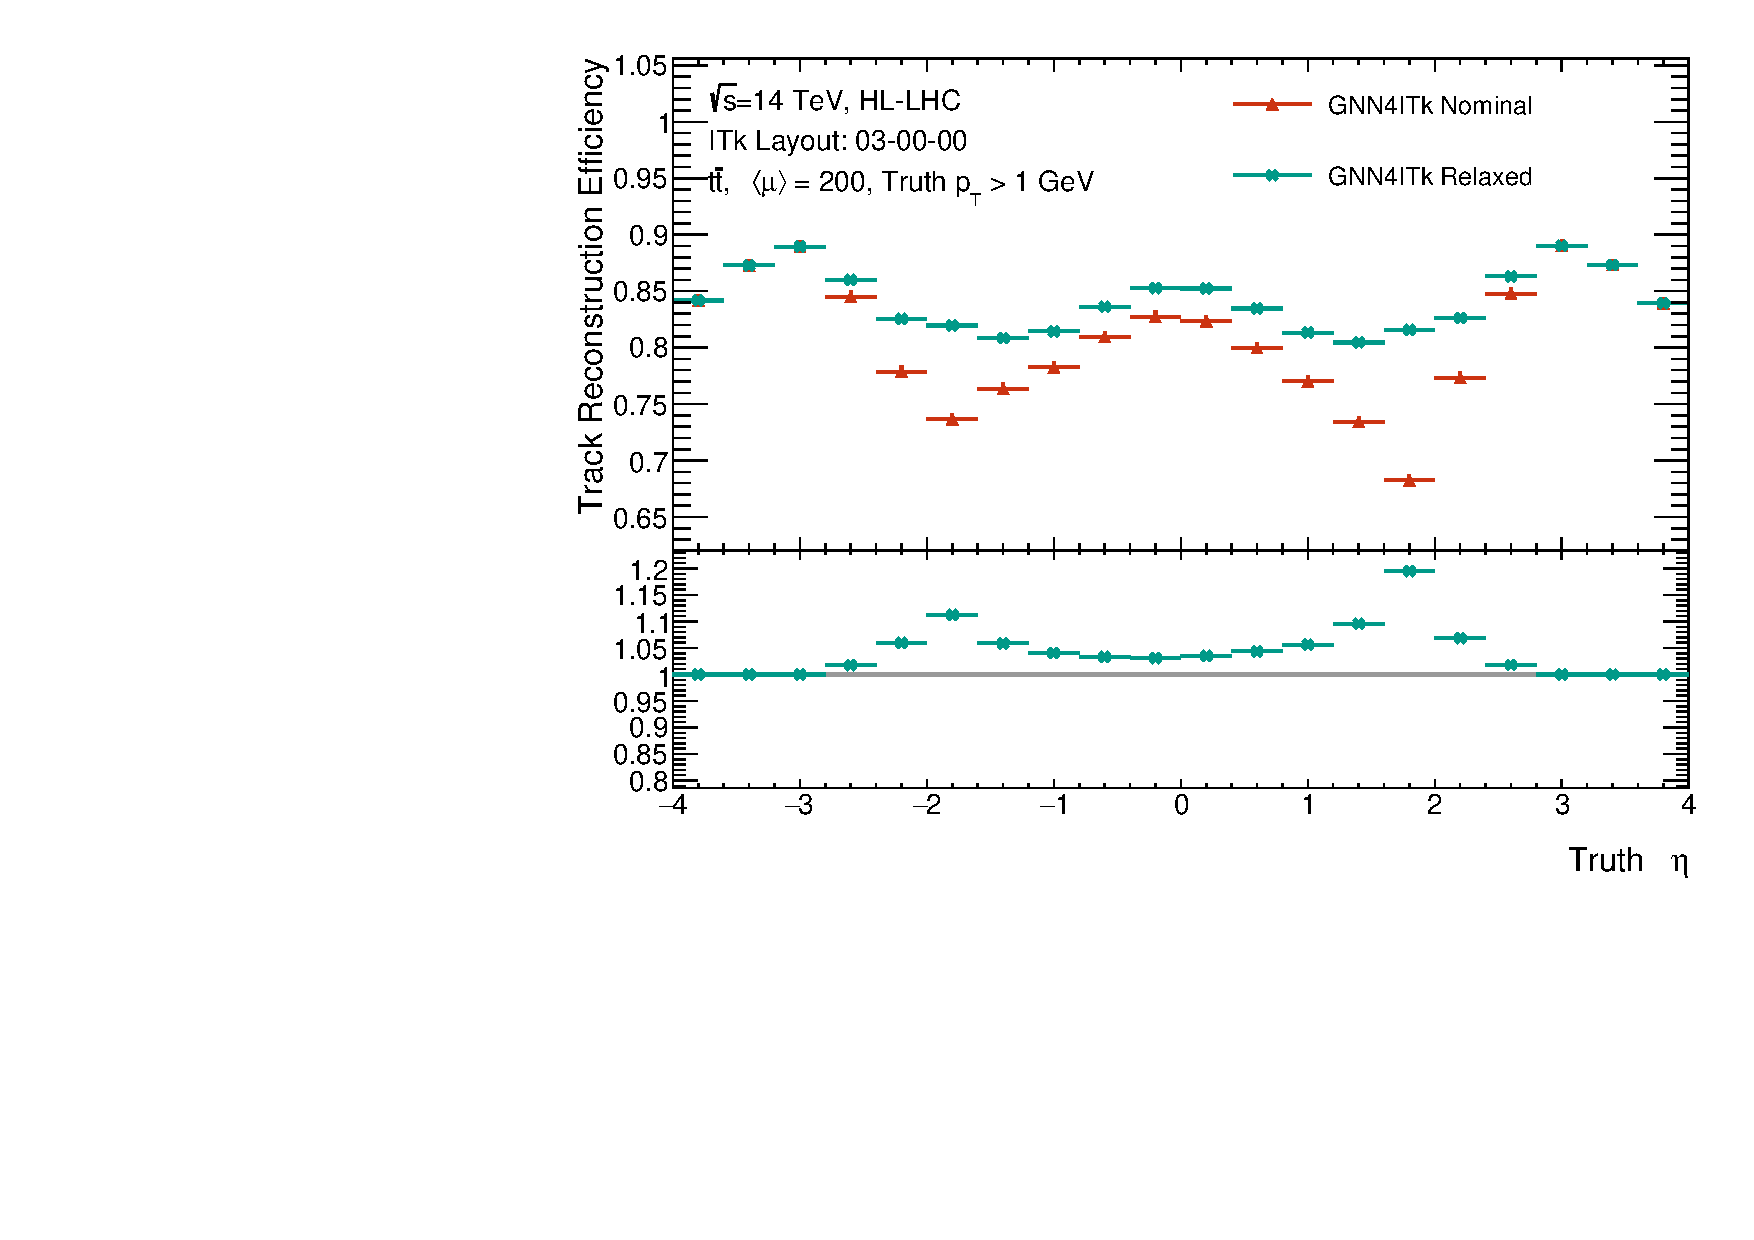
\includegraphics[width=\textwidth]{figures/nominal-vs-relaxed-cuts/Efficiency/efficiency_vs_eta.pdf}
    \caption{}
    \label{subfig:nominal-vs-relaxed-eff}
\end{subfigure}
\begin{subfigure}{0.49\textwidth}
    \centering
    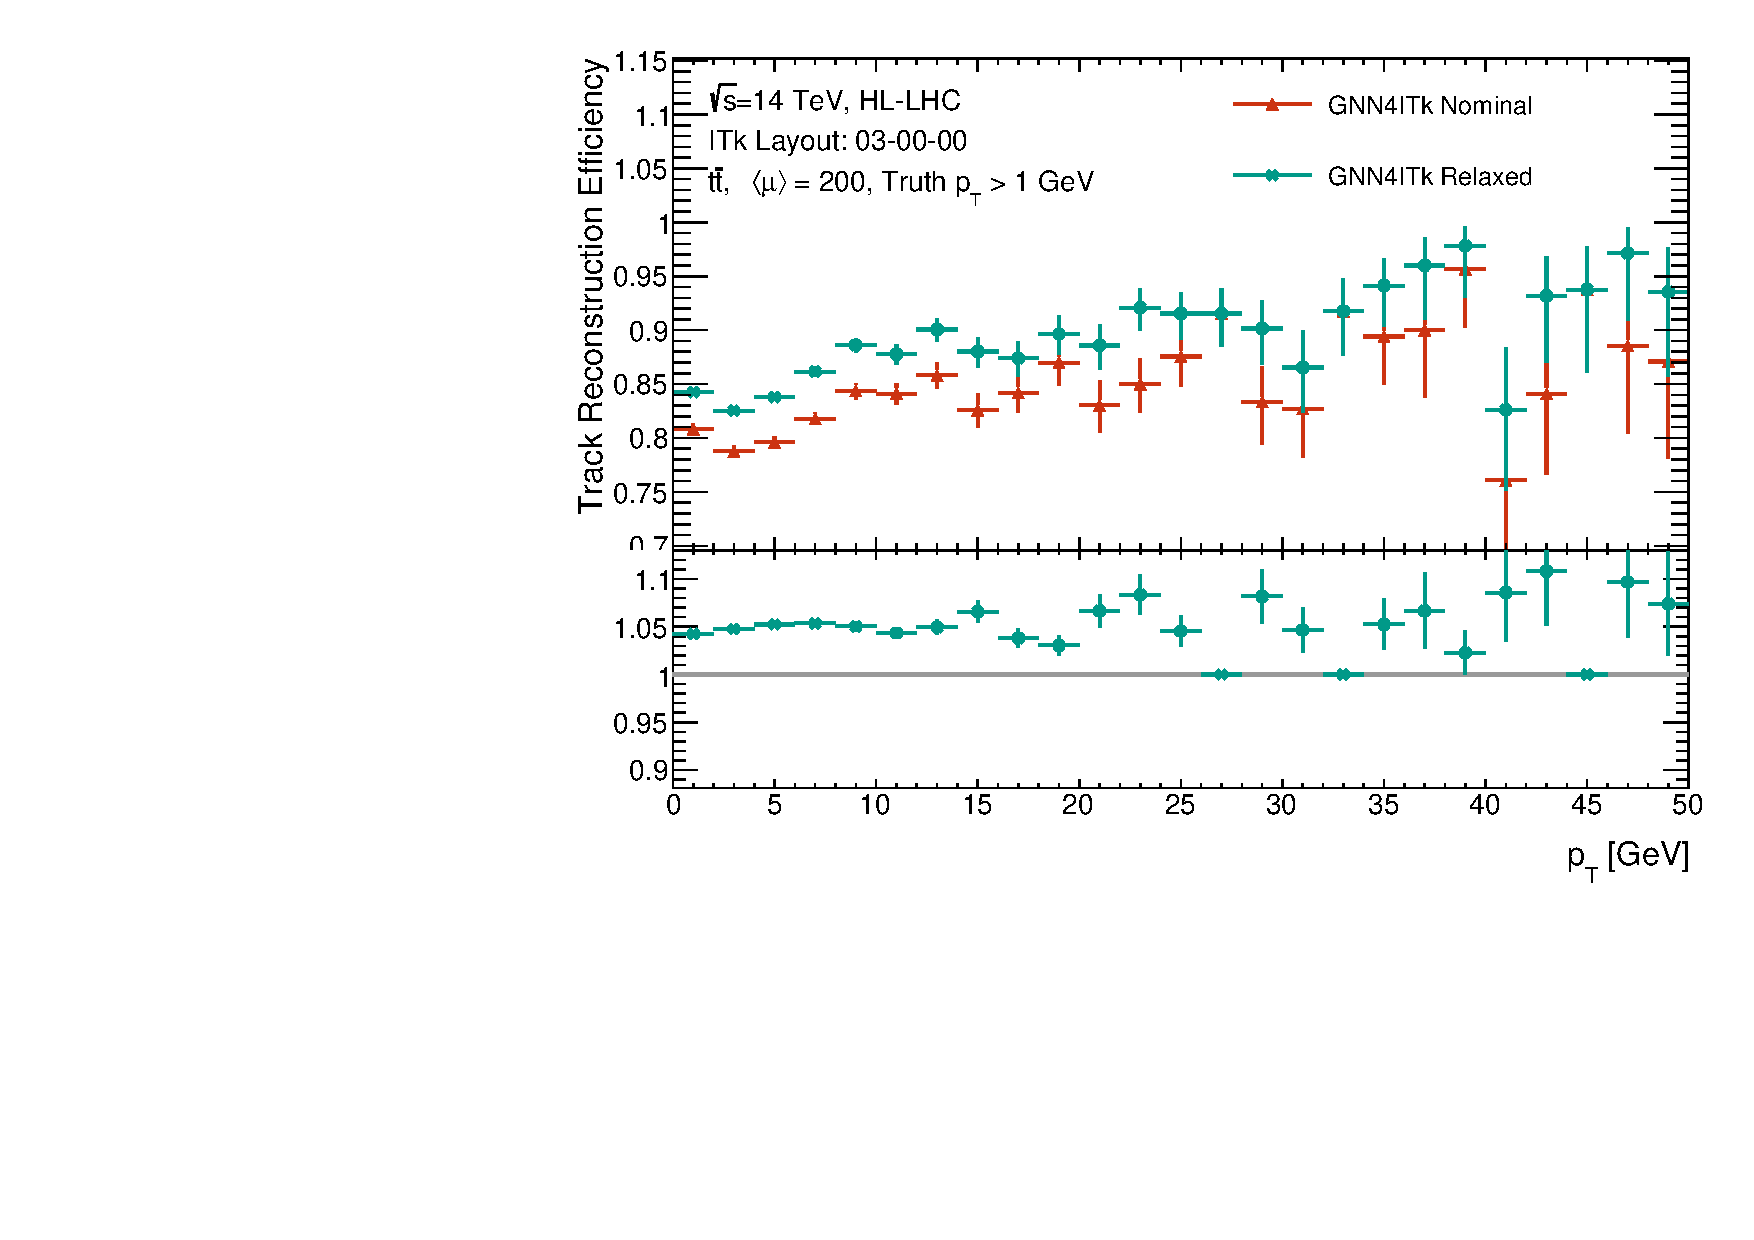
\includegraphics[width=\textwidth]{figures/nominal-vs-relaxed-cuts/Efficiency/efficiency_vs_pt.pdf}
    \caption{}
    \label{subfig:nominal-vs-relaxed-eff-pt}
\end{subfigure}
\begin{subfigure}{0.49\textwidth}
    \centering
    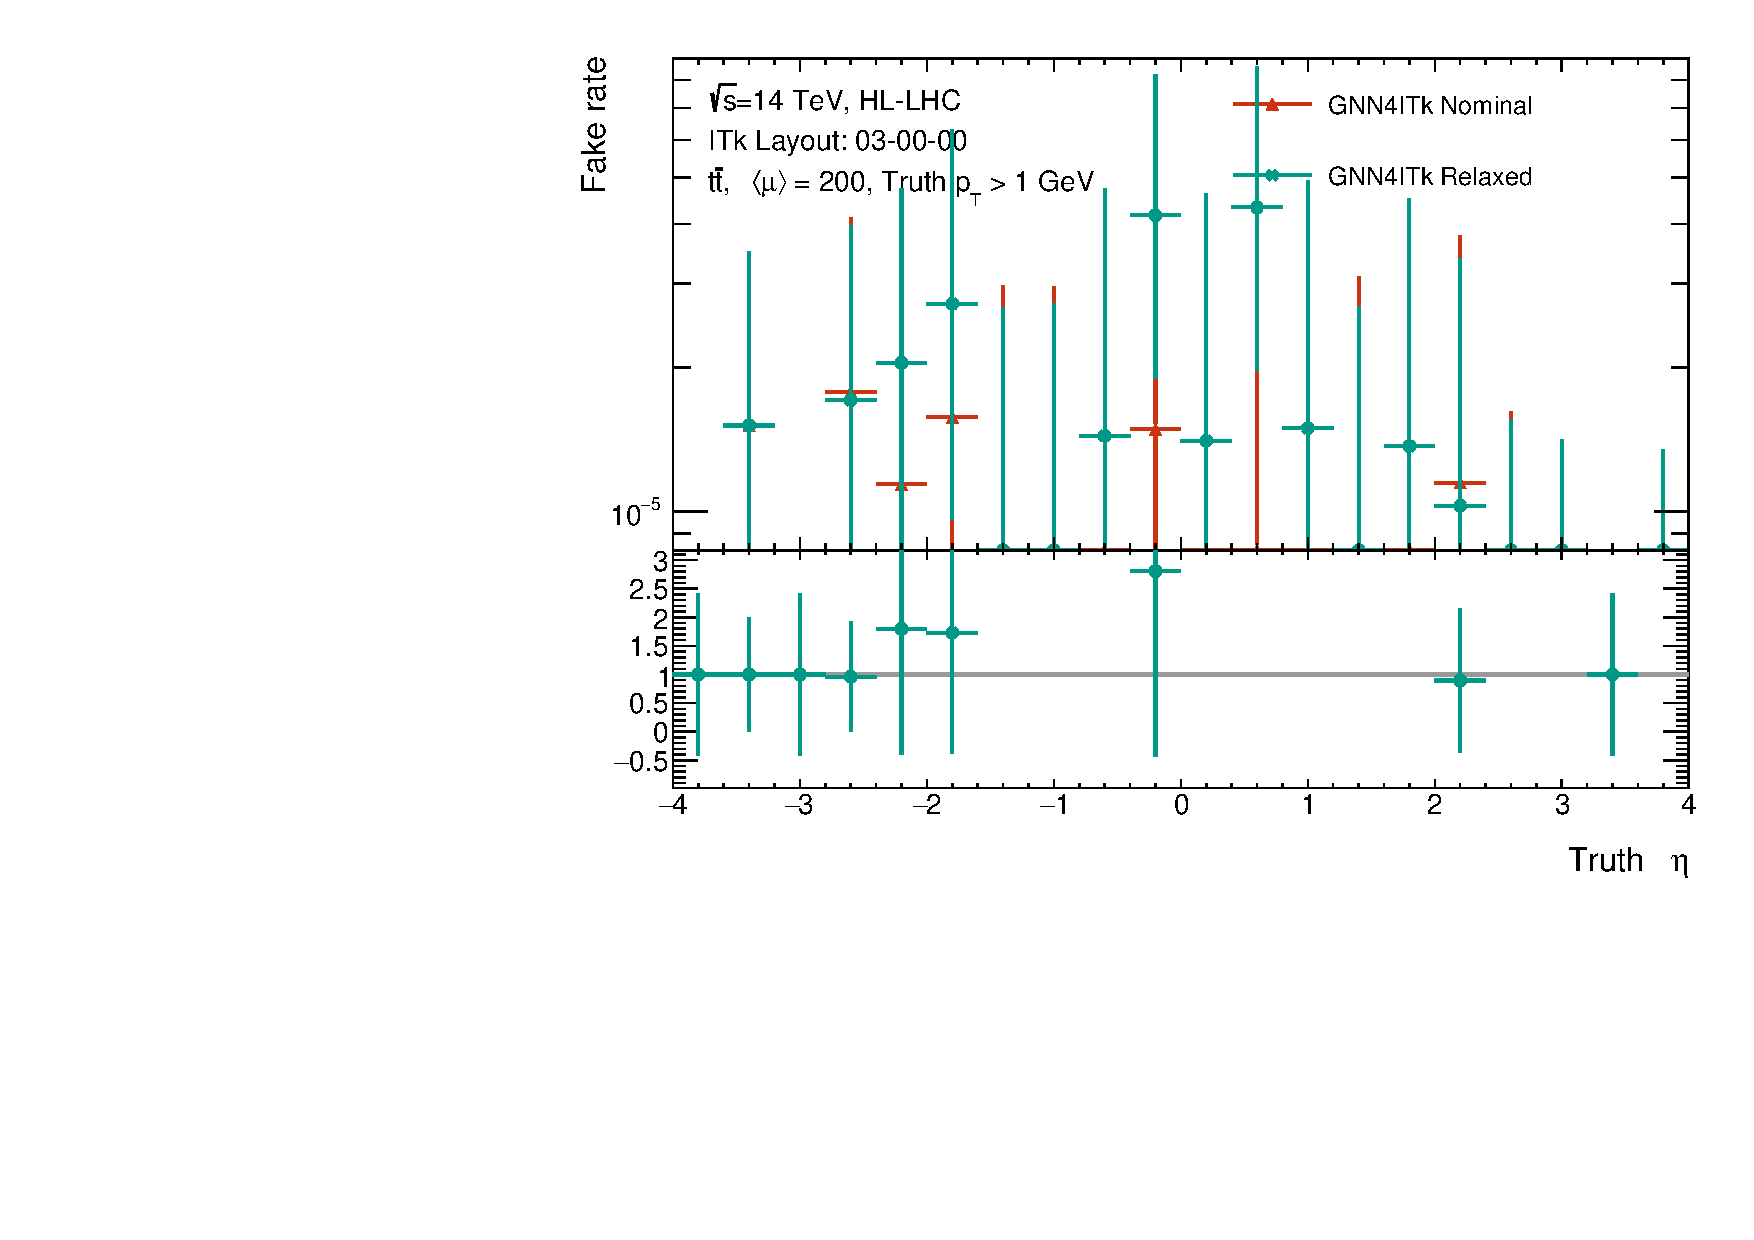
\includegraphics[width=\textwidth]{figures/nominal-vs-relaxed-cuts/FakeRate/fakerate_vs_eta.pdf}
    \caption{}
    \label{subfig:nominal-vs-relaxed-fake}
\end{subfigure}
\begin{subfigure}{0.49\textwidth}
    \centering
    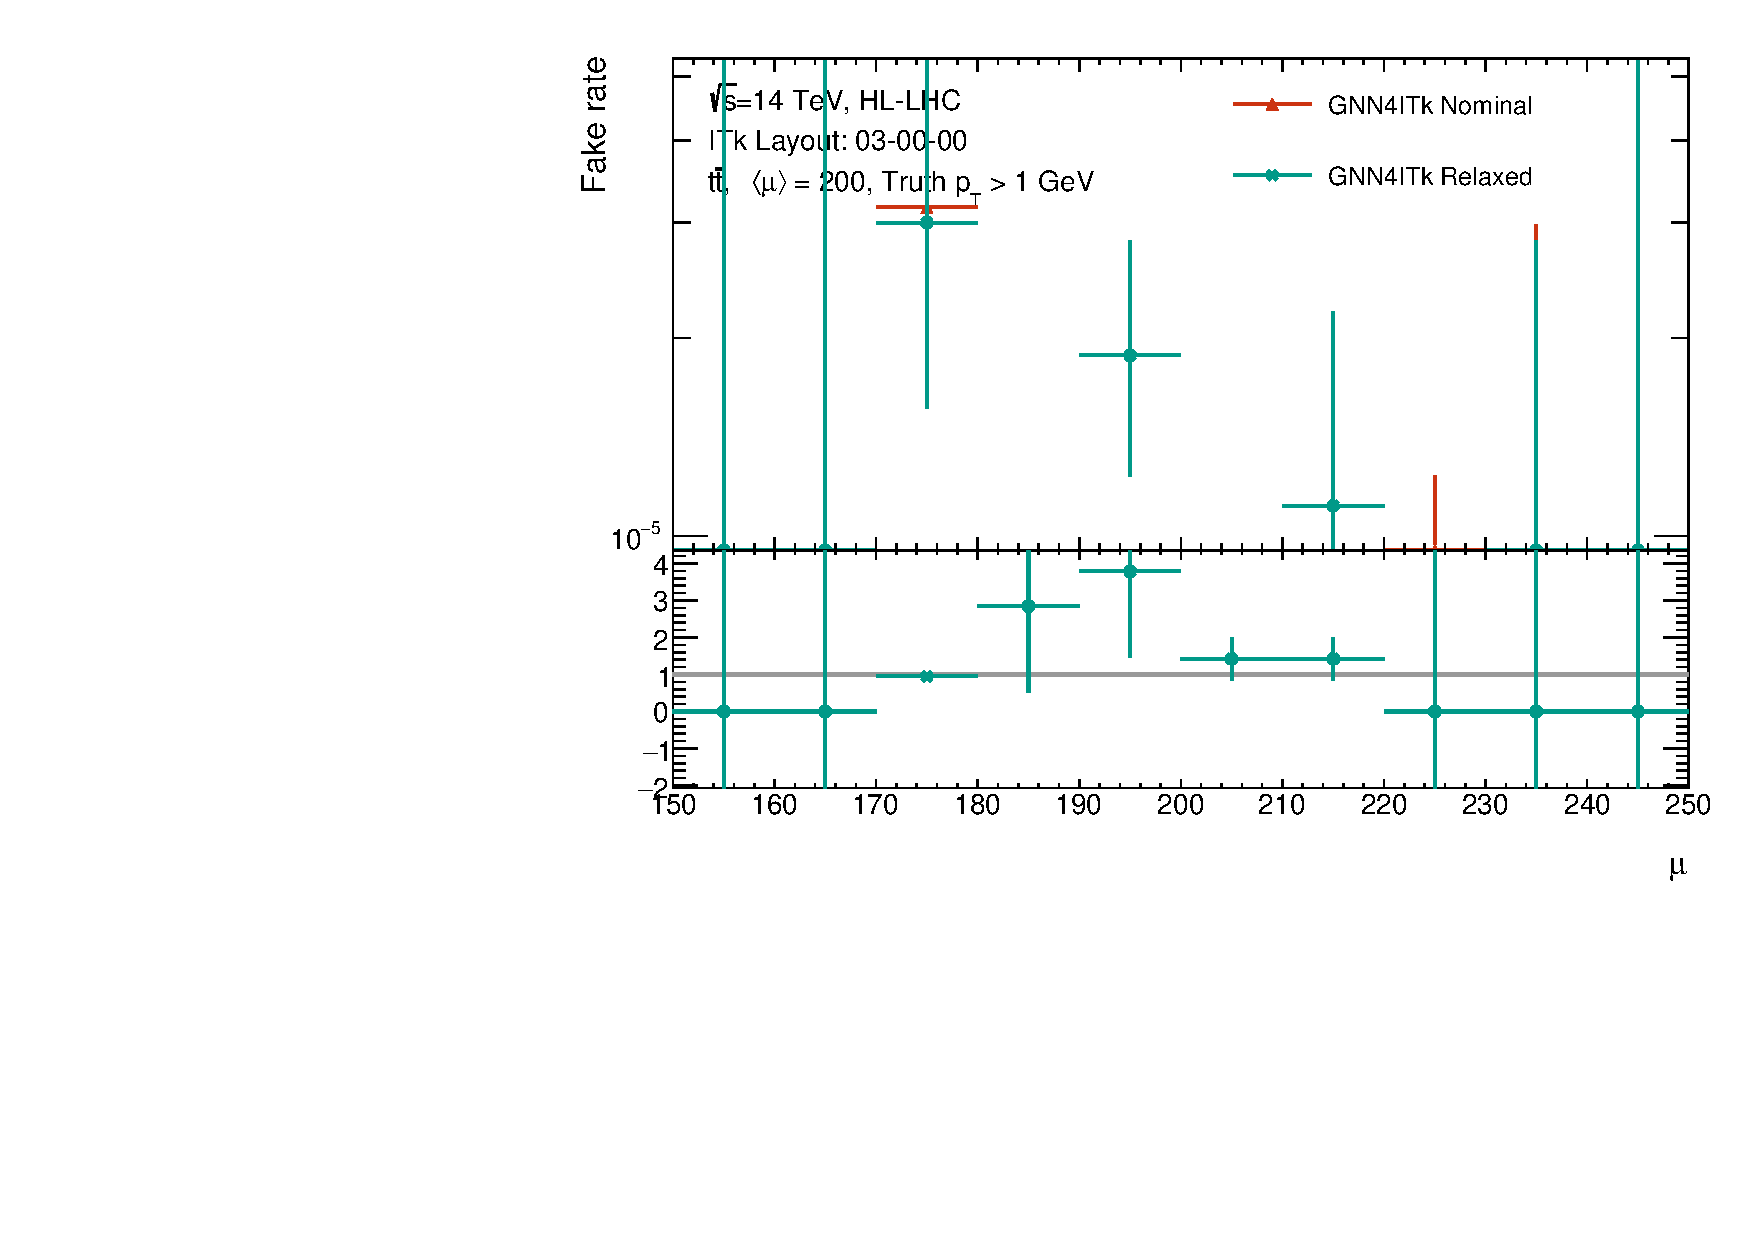
\includegraphics[width=\textwidth]{figures/nominal-vs-relaxed-cuts/FakeRate/fakerate_vs_mu.pdf}
    \caption{}
    \label{subfig:nominal-vs-relaxed-fake-mu}
\end{subfigure}
    \caption{A comparison of the GNN-based track candidates selected by the nominal and the relaxed criteria in representative performance metrics. Top plots show the efficiency as functions of the truth pseudorapditiy $\eta$ (a) and transverse momentum \pT (b). Bottom plots show the rate of fake tracks as functions of $\eta$ (c) and the pile-up level $\mu$ (d).}
    \label{fig:nominal-vs-relaxed}
\end{figure}

Efficiency and fake rate are typically in a trade-off relationship, such that to increase efficiency, one often admit more track candidates by loosening some selection criteria, potentially allowing those constructed from randomly associated hits. 
Fake tracks at best consume extra computing resources and at worse introduce bias to event- and object-level parameters, such as the missing transverse momentum $p_{T,miss}$ which is estimated as the compliment of the total visible transverse momentum. 
As parameter biases from the tracker accumulate throughout the reconstruction chain, it is particularly important to control the number of fake tracks.
In fact, the nominal cuts in table \ref{tab:track-reco-cuts} are optimized with a primary objective of limiting the fake rate~\cite{Aad_2025}.

Despite the increased efficiency, no explosion in the number fake tracks is observed with the relaxed cuts. 
Shown in figure \ref{subfig:nominal-vs-relaxed-fake}, the average fake rate under both the nominal and the relaxed selections is of $\mathcal{O}(10^{-5})$, i.e. every 10000 track candidates contain $\mathcal{O}(1)$ fake track.
Considering that the track builder produces about 2000 tracks per event, this fake rate implies that both sets of cuts can filter all fake candidates in the majority of events.
Table \ref{tab:integrated-fake} shows the total number of fake candidates among 1000 test $t\bar{t}$-events produced by the GNN- and CKF-based track builders under the two sets of selections. 
While the relaxed cuts increase the number of fake by a factor of 9 for the CKF, only a factor of 2 is observed for the GNN, in addition to its small absolute values.
Therefore, for the CKF, requiring track candidates to satisfy the requirements in table \ref{tab:track-reco-cuts} is \textit{essential} to limit fake tracks and maintain good efficiency. 
On the other hand, for the GNN4ITk, a relaxation in the minimum number of hits and the maximum number of holes in the strip region ($\abs{\eta}<2.6$) is necessary to cope with the input hit inefficiency, yet still guarantees low fake rate, thus achieving an optimal performance.

\begin{table}[h!]
    \centering
    \begin{tabular}{|l|c|c|} \hline
        Track selection & GNN4ITk & CKF \\ \hline
        Nominal & 11 & 130 \\
        Relaxed & 22 & 1205 \\ \hline
    \end{tabular}
    \caption{The total number of reconstructed tracks by the GNN4ITk and the CKF chains having matching probability less than 0.5 over 1000 $t\bar{t}$ events.}
    \label{tab:integrated-fake}
\end{table}

These factors when considered together justify the evaluation of GNN-based tracking performance at relaxed selections, and the CKF-based performance at the nominal selections. 
In light of this discussion, we propose to apply a minimally modified set of cuts, shown in table \ref{tab:track-reco-cuts-semi-relaxed} to all tracks built by the GNN-based algorithm.

\begin{table}[h!]
    \centering
    \begin{tabular}{|l|c|c|c|} \hline
       \multirow{2}{*}{Requirements}  & \multicolumn{3}{c|}{Pseudorapidity interval} \\ \cline{2-4}
         & $\abs{\eta} \le 2.0 $ & $2.0< \abs{\eta} \le 2.6$ & $2.6 < \abs{\eta} < 4.0 $ \\ \hline
         {Number of clusters} & $\ge 7$ & $\ge 7$ & $\ge 7$ \\
         {Number of holes} & $\le 4$ & $\le 4$ & $\le 2 $ \\
         Number of pixel clusters & $\ge 1$ & $\ge 1$ & $\ge 1$ \\
         \pT [MeV] & $> 900$ & $>400$ & $>400$ \\
         $\abs{d_0}$ [mm] & $< 2.0$ & $<2.0$ & $<10.0$ \\
         $\abs{z_0}$ [cm] & $< 20.0$ & $<20.0$ & $<20.0$ \\
         \hline     
    \end{tabular}
    \caption{Minimally modified selections adapted to GNN-based tracks. Modified criteria with respect to those in table \ref{tab:track-reco-cuts} are highlighted in boldface. The rest is identical to reference \cite{Aad_2025}.}
    \label{tab:track-reco-cuts-semi-relaxed}
\end{table}

\subsection{Reconstruction efficiency}
\label{subsect:tracking-efficiency}

In this section, we compare the reconstruction efficiency of the three variants of the GNN-based algorithm to that of the CKF.
Track candidates produced by the former are required to pass the quality cuts in table \ref{tab:track-reco-cuts-semi-relaxed}, and those produced by the latter are required to pass the cuts in table \ref{tab:track-reco-cuts}. 
The tracking efficiency as functions of the truth $\eta$ and \pT are respectively shown in figures \ref{subfig:tracking-eff-eta} and \ref{subfig:tracking-eff-pt}. 
The bottom plot in each figure shows the ratio between each of the GNN-based curves to the CKF-based curve.

\begin{figure}[h!]
\centering
\begin{subfigure}{0.65\textwidth}
    \centering
    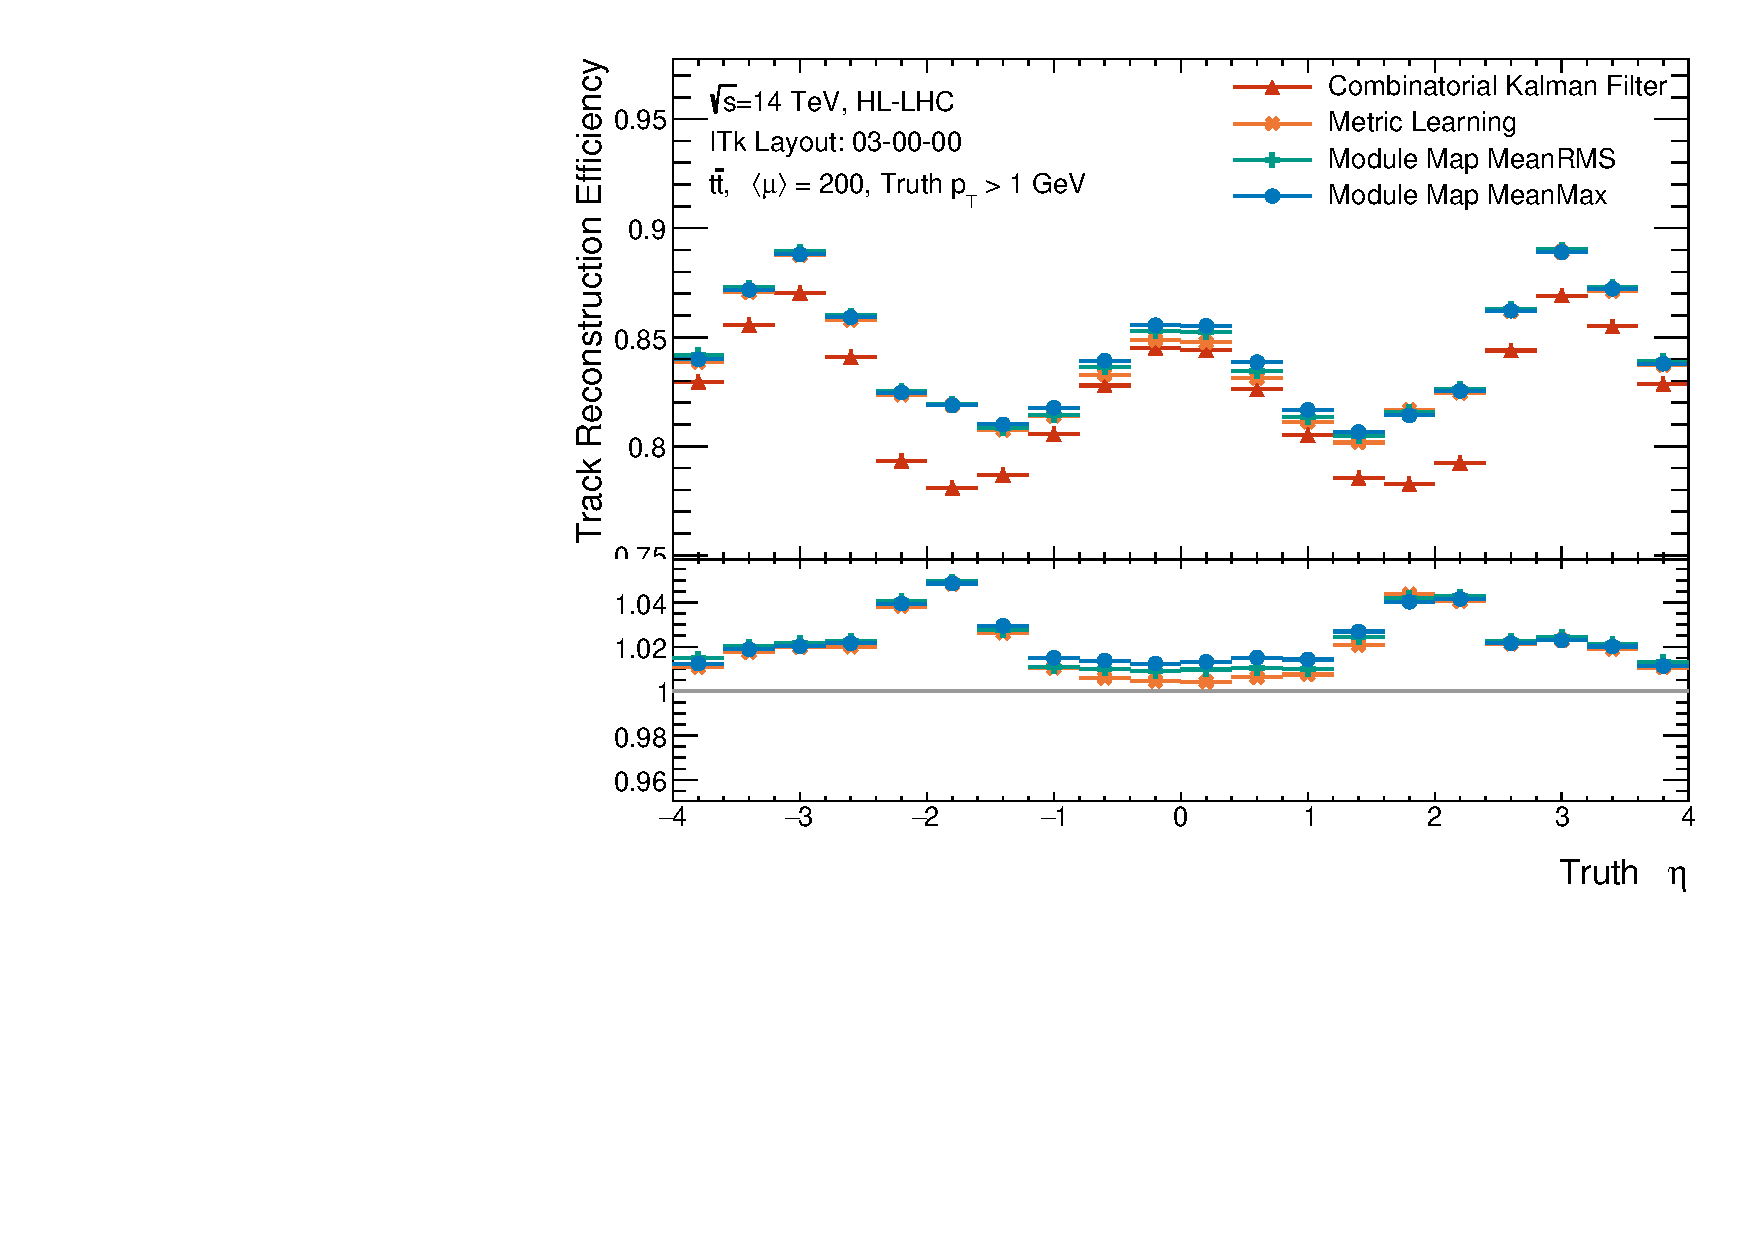
\includegraphics[width=\textwidth]{figures/ckf-gnn/Efficiency/efficiency_vs_eta.pdf}
    \caption{}
    \label{subfig:tracking-eff-eta}
\end{subfigure} 
\begin{subfigure}{0.65\textwidth}
    \centering
    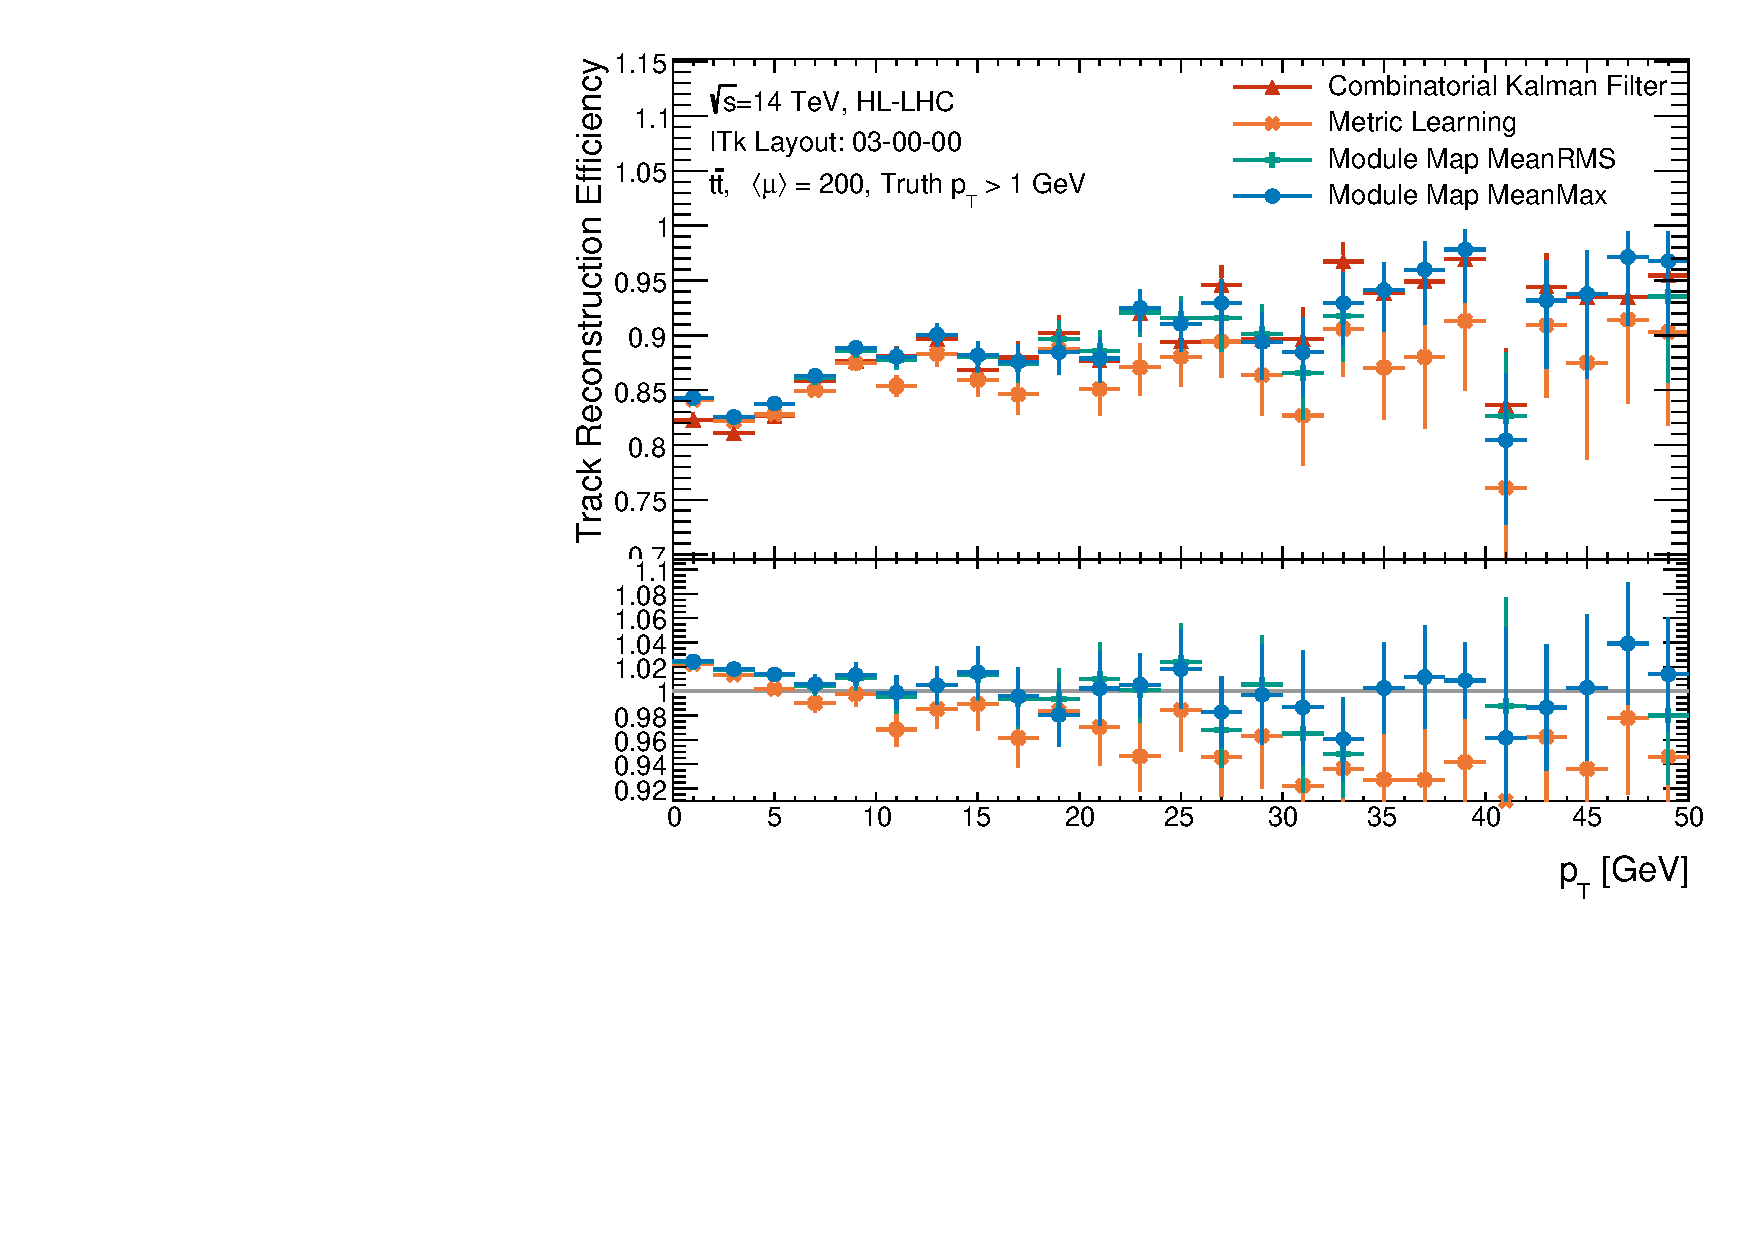
\includegraphics[width=\textwidth]{figures/ckf-gnn/Efficiency/efficiency_vs_pt.pdf}
    \caption{}
    \label{subfig:tracking-eff-pt}
\end{subfigure}
\caption{Tracking efficiency as functions of the truth pseudorapidity $\eta$ (a) and transverse momentum \pT (b). The bottom plots show the ratio of the GNN-based curves to the CKF-based curve.}
\label{fig:tracking-eff}
\end{figure}

The tracking efficiency varies as a function of truth pseudorapidity.
All reconstruction algorithms reache the maximum efficiency at $\abs{\eta}=0$ and $\eta=3.0$, and minimum at $\abs{\eta}=1.8$, symmetric around $\eta=0$
These variations are strongly correlated to the detector material encountered by the particle on its path, illustrated on figure \ref{subfig:rad-len-to-reco}. 
The total radiation length traversed by a particle before reaching the minimum number of hits to be reconstructible is lowest at $\abs{\eta}=0$ and $\abs{\eta}=3.0$ 
and peaks at $\abs{\eta}=1.5$. 
Since material effects randomly direct the real trajectory away from an ideal helix, particles travelling through more material tend to have more hits deviating considerably from 
their expected position. 
For the CKF, this means that incorporating the correct hit could significantly increase the total $\chi^2$, leading to an early termination of the hit-finding sequence and 
subsequently the track candidate failing the selection cuts.
On the other hand, trained on data which contain these ``irregular'' connections, the GNN is observed to tolerate large deviations, but the constructed track candidate could
still be ruled out by the global $\chi^2$ fit.

Among the GNN-based trackers, the best efficiency is observed in the {{Module Map MinMax}} variant, followed closely by the {{MeanRMS}} variant.
All three variants yield similar efficiency at low transverse momentum ($\pT<5$ GeV), but start to diverge at high \pT.
The {{Metric Learning}} variant is slightly less efficient than the Module Map variants for $\pT > 5$ GeV.
On the pseudorapidity spectrum, it has lower efficiency in the strip barrel in the range $\abs{\eta}<1$, but otherwise identical to the other GNN-based variants.
These observations are explain by the fact that high-\pT particles are more likely to have small pseudorapditiy and concentrate in the barrel region.
% Particles with a large transverse momentum are more likely to be concentrated in the central barrel, i.e. having small pseudorapidity. 
Graph construction using the Metric Learning is less efficient than the Module Map at high \pT, as shown in figure \ref{subfig:filter-eff-eta}, and the inefficiency accumulates throughout the pipeline,
leading to the observed degradation in tracking efficiency. 
% Consequently for the former method, the efficiency relatively degrades with increasing \pT, and, since large-\pT particles populates low $\abs{\eta}$, towards the central region.

All variants of the GNN4ITk algorithm produce tracking efficiency exceeding that of the CKF when plotted as a function of $\eta$, in which each bin is the conditional efficiency averaged over all particle momenta. 
On the \pT spectrum, however, it is clear that the improvement is not evenly distributed. 
All of the efficiency improvement occurs on particles with low \pT, as seen on the ratio plot of figure \ref{subfig:tracking-eff-pt}, the performance at high \pT is largely similar to that of the CKF.
High-\pT particles are rare, as they commonly originate from the hard-scattering collision, and concentrate around the barrel region.
The absence of efficiency improvement at high \pT partially explains the comparatively smaller efficiency boost near $\eta=0$. 
In contrast, low-\pT particles constitute the majority of target particles, orders of magnitude more abundant than their high-\pT counterparts, and are distributed quite evenly throughout the detector, which explains the excess efficiency in all $\eta$ bins on figure \ref{subfig:tracking-eff-eta}. 

Though not simply related, tracking efficiency is determined by the edge-level efficiency encountered the results of previous chapters.
The impact of the uneven \pT distribution in training data on edge-level performance was already seen in section \ref{sect:filter-results}. 
All models in the GNN4ITk are trained on data which predominantly features low-\pT tracks. 
They learn to minimize the classification loss of true edges from these tracks, possibly at the expense of the other less abundant particles.
As discussed in section \ref{subsect:ignn-result}, increasing the weight of high-\pT edges in the loss function proves ineffective.
For now, despite the degradation in the edge efficiency, the efficiency of the GNN-based tracker at high momentum matches that of the CKF in absolute terms. 
Increasing the per-edge performance of the pipeline at high \pT is a priority for future work.

% The tracking efficiency as functions of the particle's pseudorapidity $\eta$ and transverse momentum \pT are respectively shown in figures \ref{subfig:tracking-eff-eta} and \ref{subfig:tracking-eff-pt}, for tracks reconstructed by the CKF and the GNN-based algorithm using graphs created by the Metric Learning and Module Map MeanRMS methods. 
% The bottom plot in each figure shows the ratio between each of the GNN-based curves to the CKF-based curve.

% Figures  respectively show the tracking efficiency as functions of the particle's pseudorapidity $\eta$ and transverse momentum \pT.
% \newpage
% \begin{sidewaysfigure}
% \centering
% \begin{subfigure}[b]{0.45\textwidth}
%     \centering
%     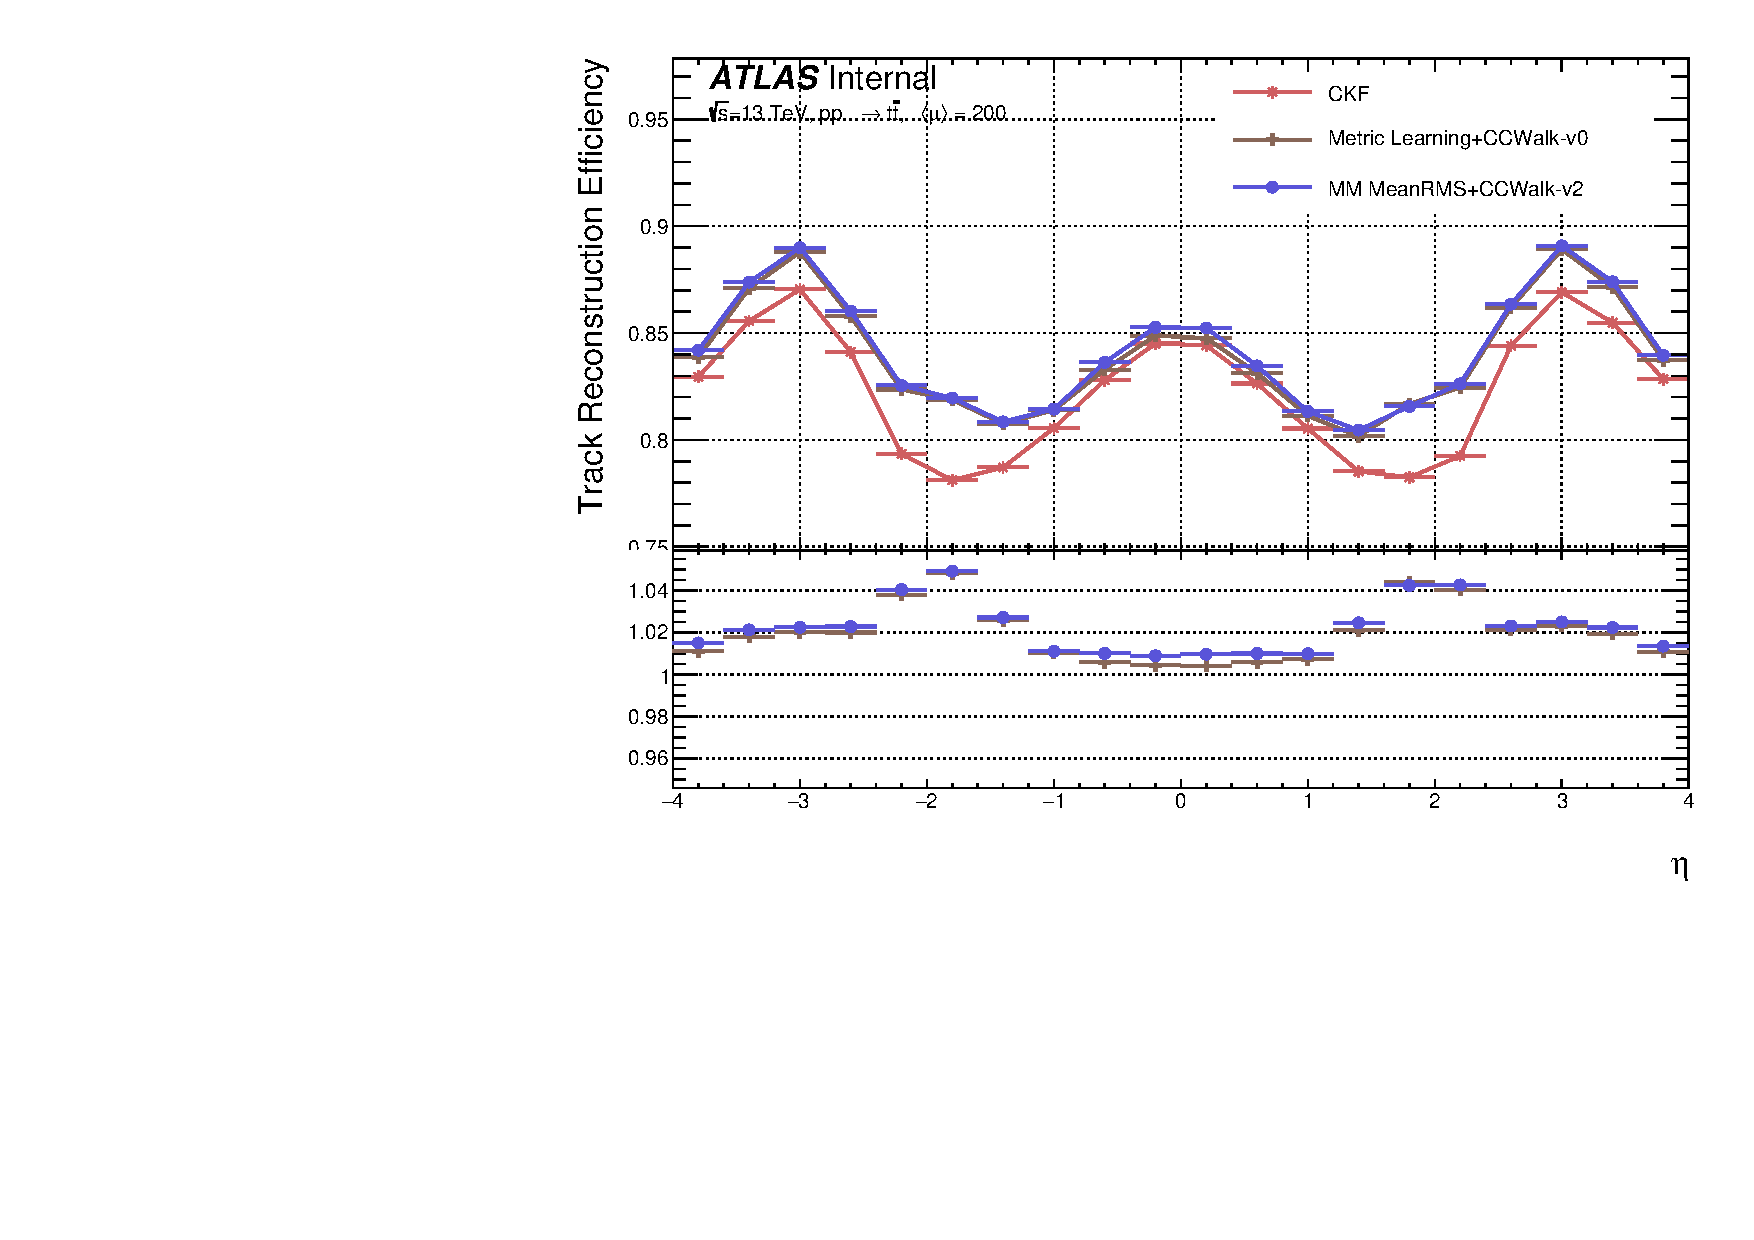
\includegraphics[width=\textwidth]{figures/Efficiency/efficiency_vs_eta.pdf}
%     \caption{Vs eta}
%     \label{subfig:tracking-eff-eta}
% \end{subfigure}
% \begin{subfigure}[b]{0.45\textwidth}
%     \centering
%     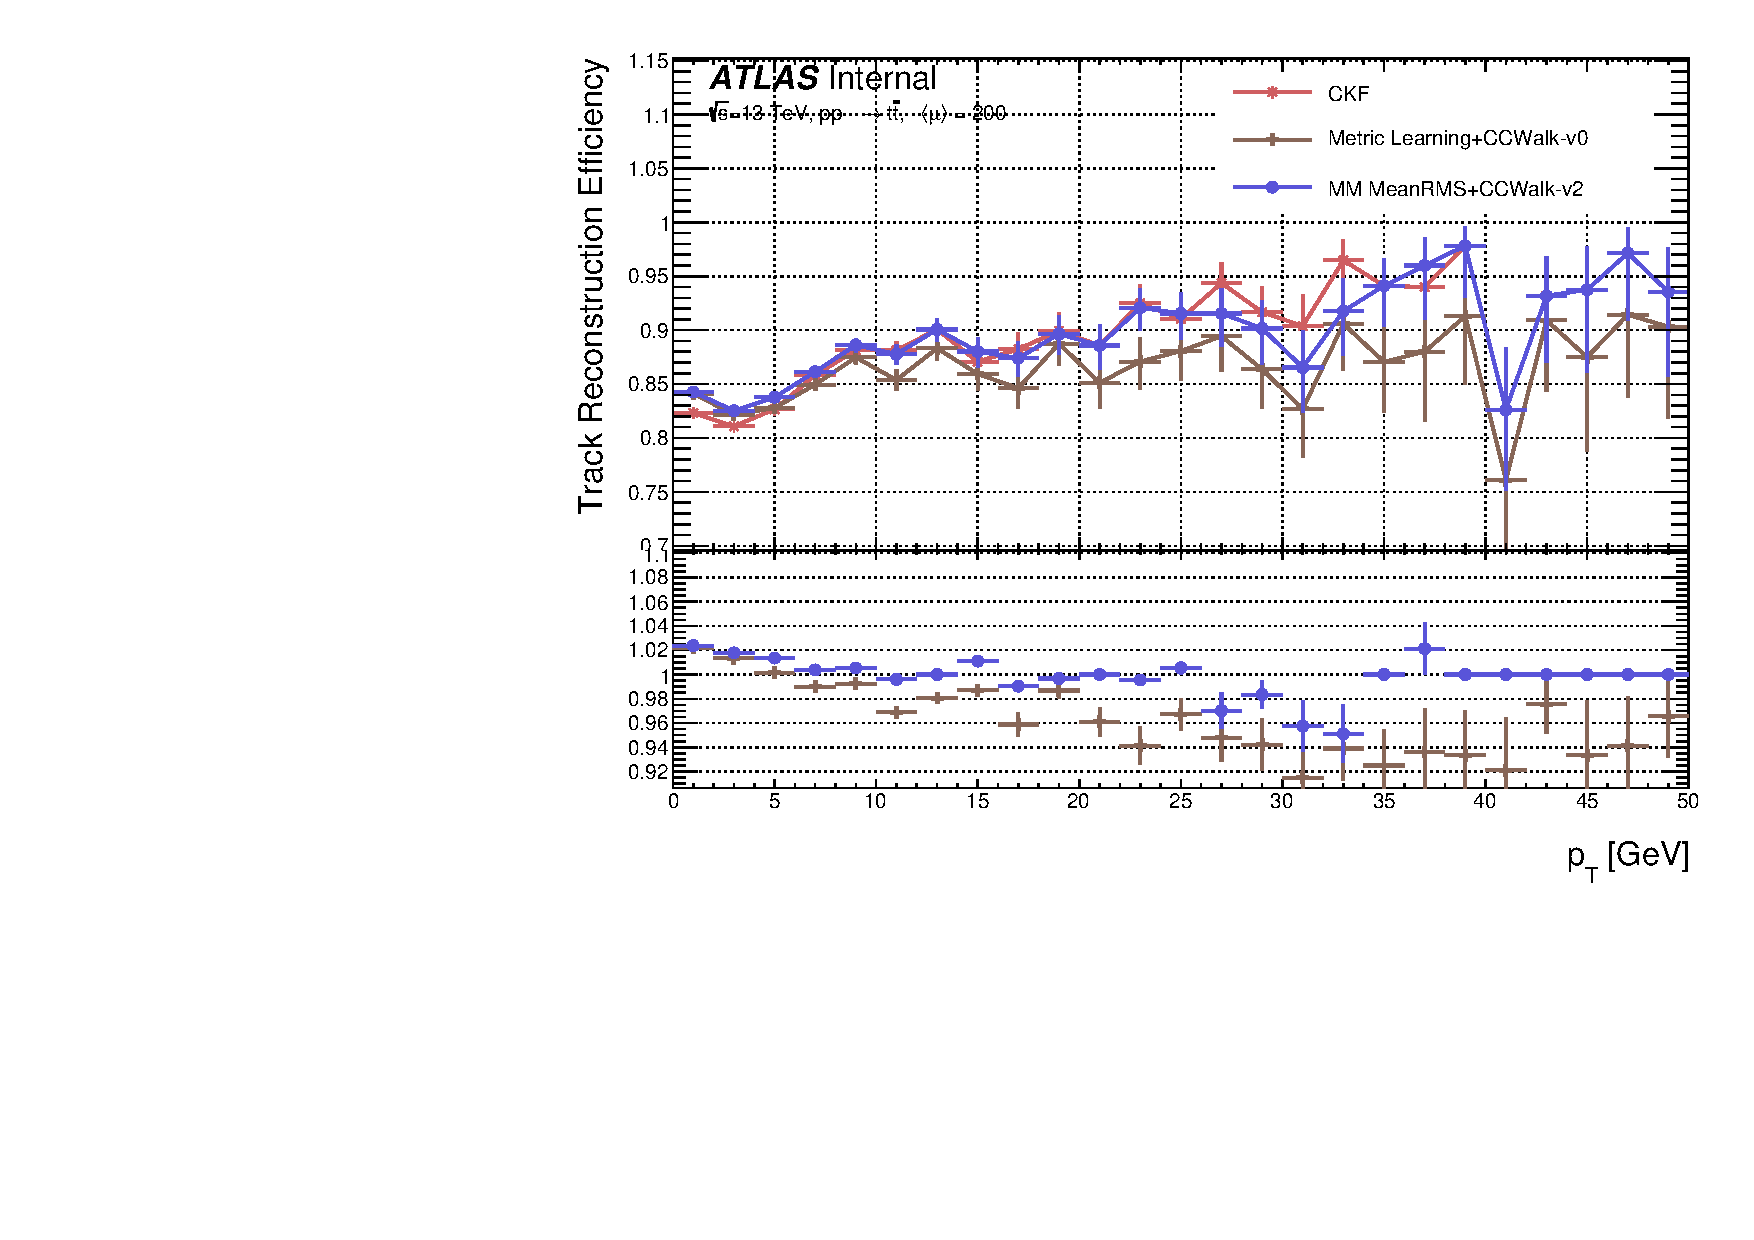
\includegraphics[width=\textwidth]{figures/Efficiency/efficiency_vs_pt.pdf}
%     \caption{vs pt}
%     \label{subfig:tracking-eff-pt}
% \end{subfigure}
% \begin{subfigure}[b]{0.45\textwidth}
%     \centering
%     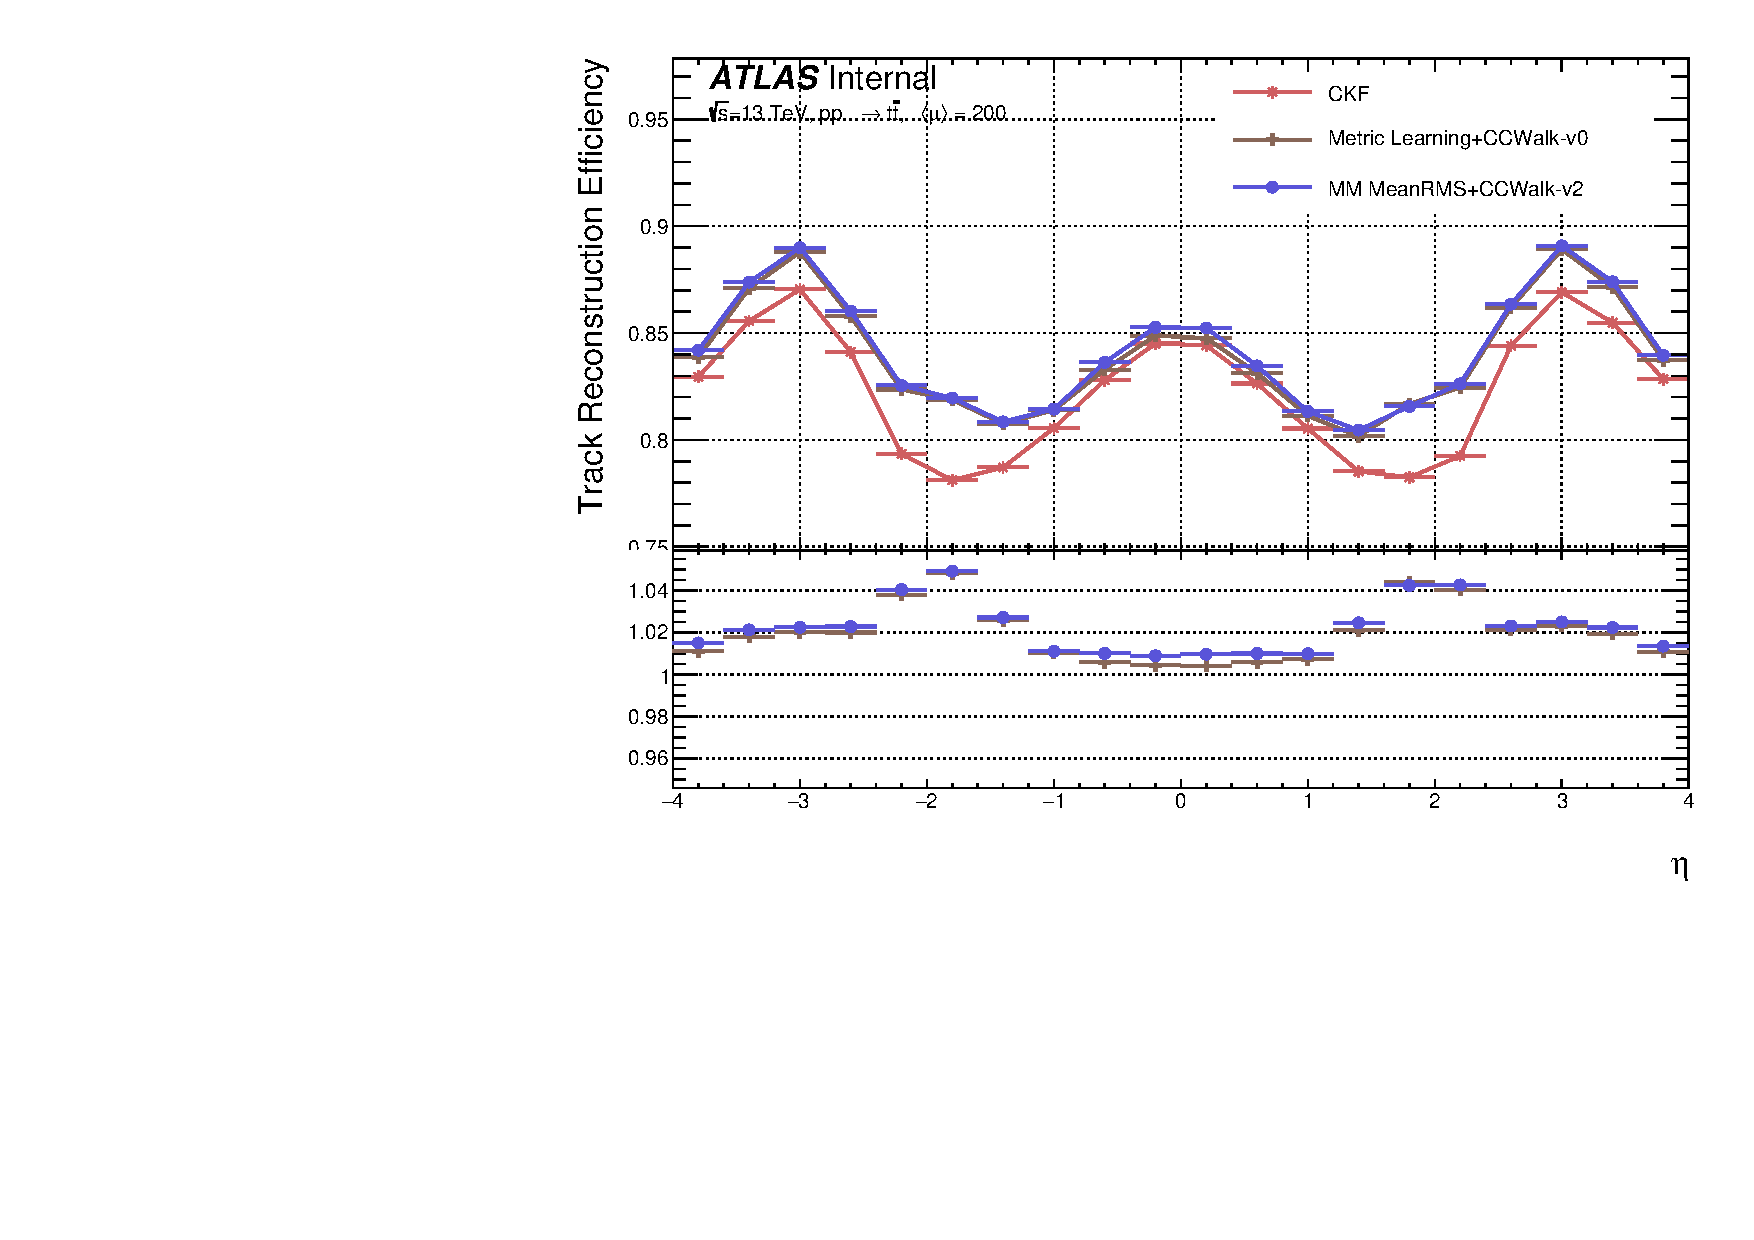
\includegraphics[width=\textwidth]{figures/Efficiency/efficiency_vs_eta.pdf}
%     \caption{Vs eta}
%     \label{subfig:tracking-eff-eta-hs}
% \end{subfigure}
% \begin{subfigure}[b]{0.45\textwidth}
%     \centering
%     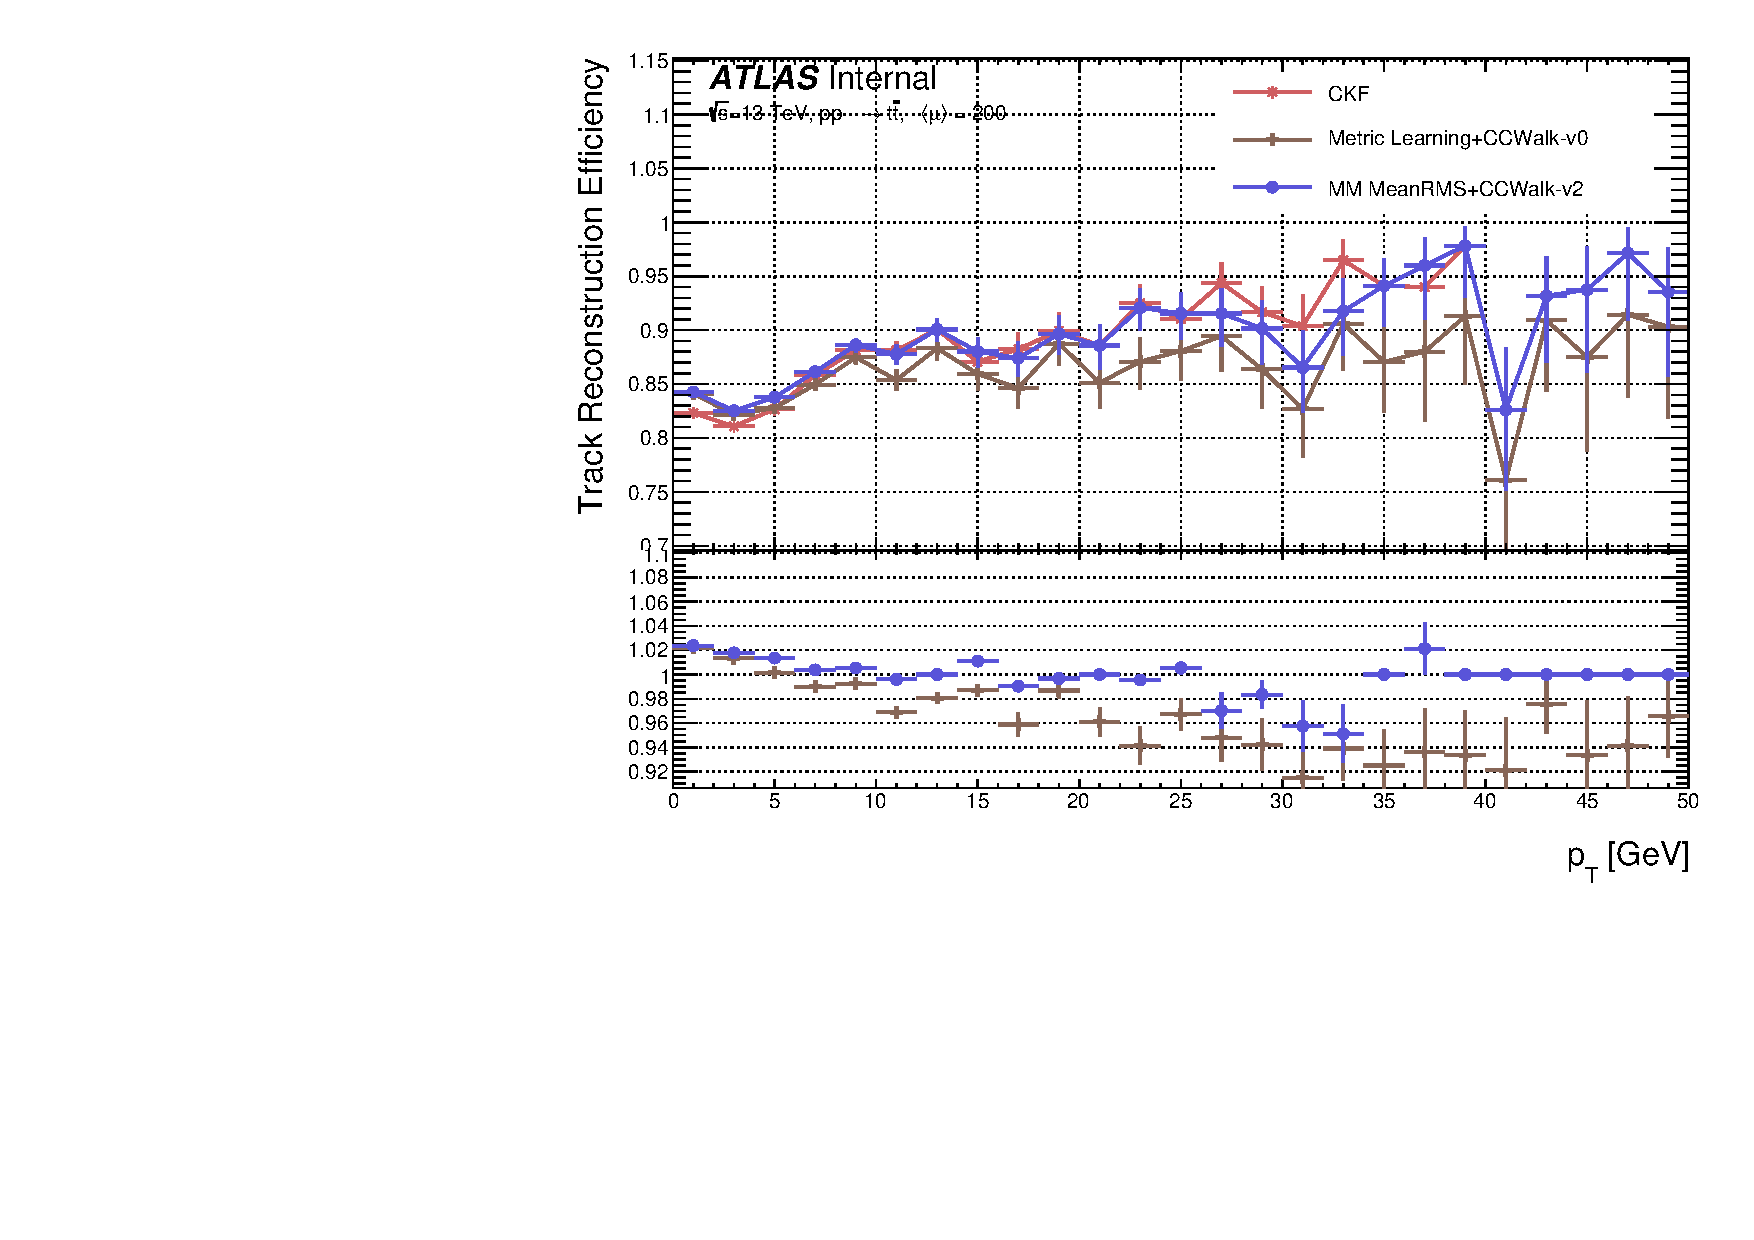
\includegraphics[width=\textwidth]{figures/Efficiency/efficiency_vs_pt.pdf}
%     \caption{vs pt}
%     \label{subfig:tracking-eff-pt-hs}
% \end{subfigure}
%     \caption{Tracking efficiency}
%     \label{fig:tracking-efficiency-eta-pt}
% \end{sidewaysfigure}

\begin{figure}[h]
    \centering
    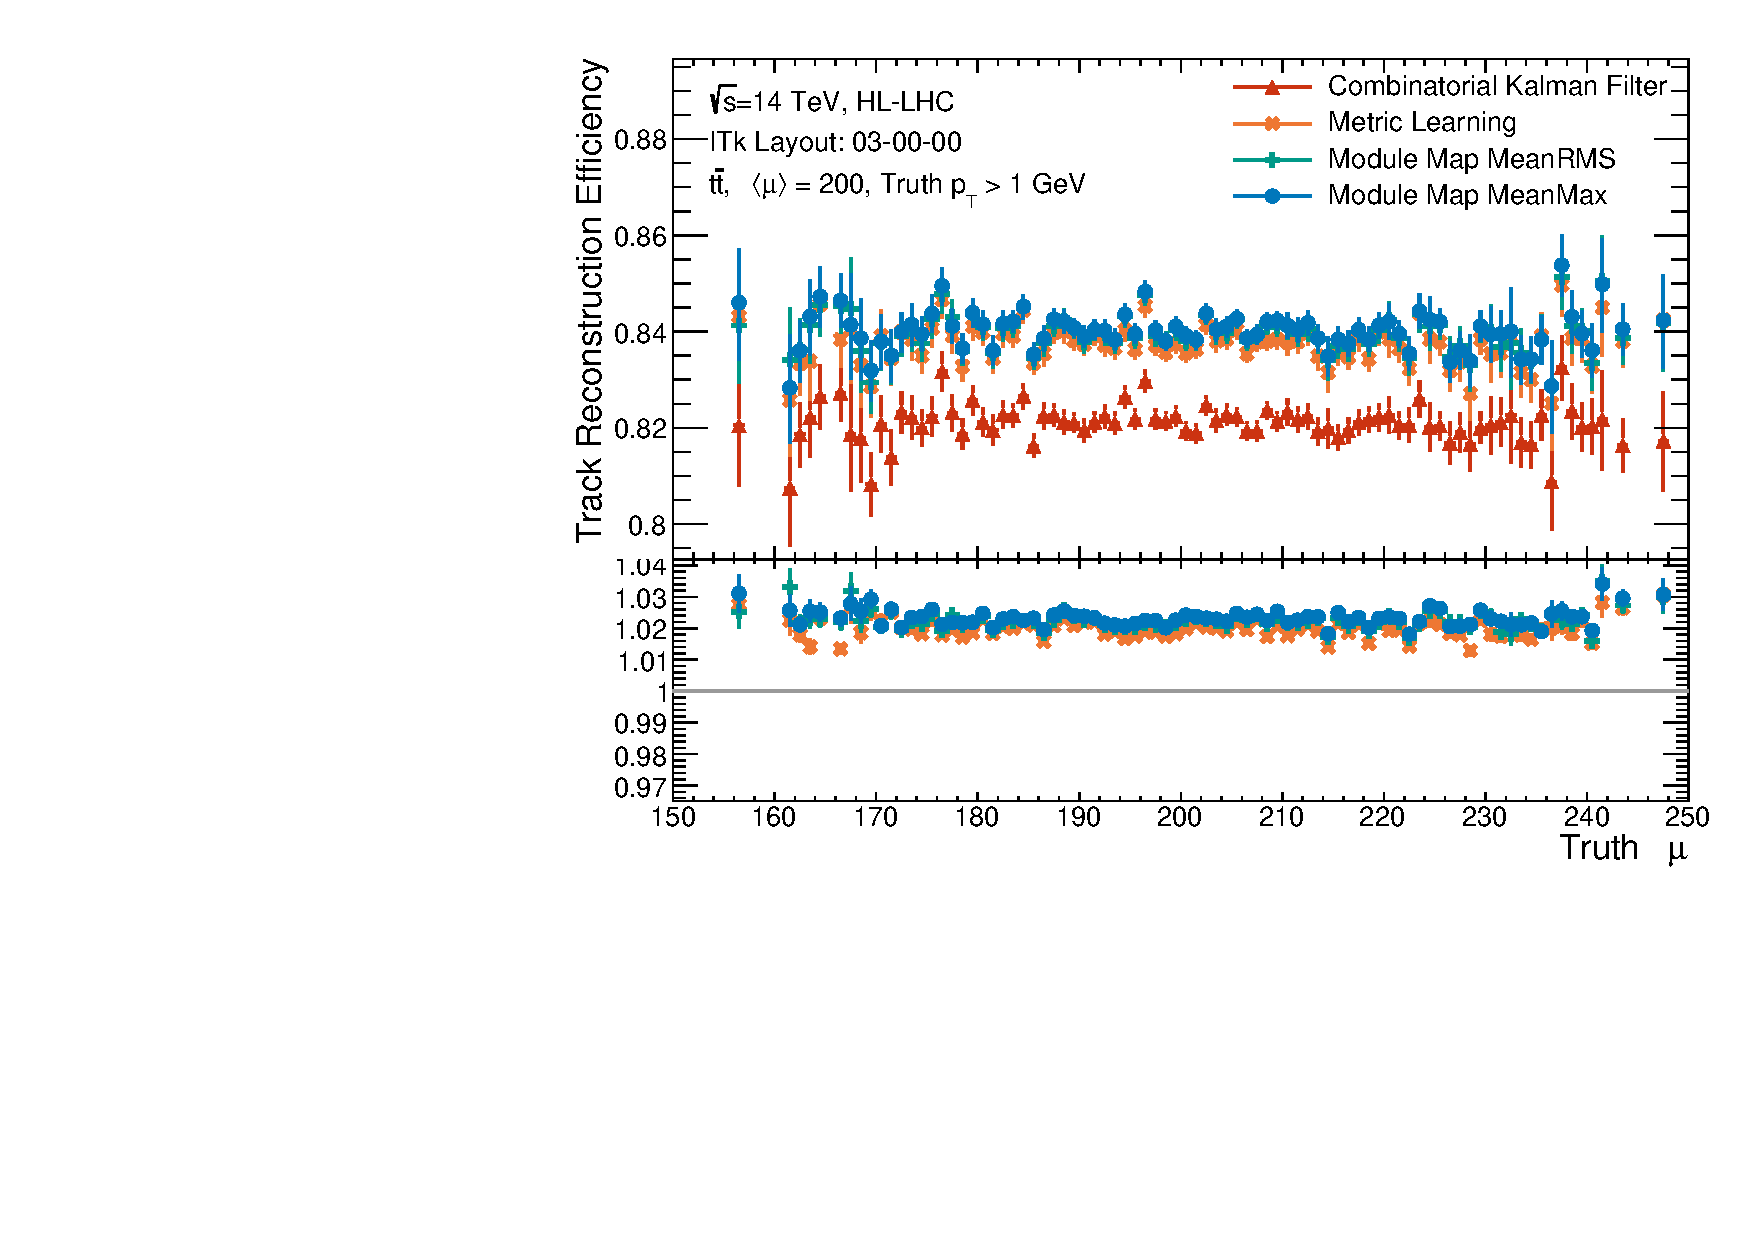
\includegraphics[width=0.65\textwidth]{figures/ckf-gnn/Efficiency/efficiency_vs_truthMu.pdf}
    \caption{Tracking efficiency as a function of the pile-up level $\expval{\mu}$. The bottom plots show the ratio of the GNN-based curves to the CKF-based curve.}
    \label{fig:tracking-eff-mu}
\end{figure}
Figure \ref{fig:tracking-eff-mu} shows the tracking efficiency as a function of truth pile-up level.
The tracking efficiency is found to be stable over a range of pile-up from $\mu=160$ to $\mu=240$. 
The GNN-based track builders are on average 84\% efficiency, while the CKF is 82\%. 
No degradation is observed with increased pile-up.

\subsection{Track fake rate}
\label{subsect:tracking-fake}

The proportion of track candidates without a matching truth particle as functions of the truth pseudorapidity and pile-up is shown in figures  \ref{subfig:tracking-fake-eta} and \ref{subfig:tracking-fake-mu}. 
While both the GNN4ITk and the CKF have fake rate order $\mathcal{O}(10^{-5})$, the former produces fewer fake tracks than the latter.
As seen in table \ref{tab:integrated-fake}, the total number of fake tracks from the GNN is approximately $1/6$ of those from the CKF.
Despite more truth particles are reconstructed by the GNN than by the CKF, evidenced by the better efficiency, only track candidates matched to these particles are created in excess. 
In other words, we achieve higher efficiency without paying the cost of building more low-quality, unassociated tracks. 
It lends support to the use of selection criteria that are adapted to a specific algorithm of interest, rather than rigidly adopting a predetermined working point optimized for a different one. 
% In the case of the GNN4ITk, many true particle tracks are uniquely reconstructed but would not be selected by the nominal selections due to the missing single clusters. 
% respectively show the tracking fake rate as functions of the particle's pseudorapidity $\eta$ and transverse momentum \pT.

\begin{figure}[h!]
\centering
\begin{subfigure}[b]{0.6\textwidth}
    \centering
    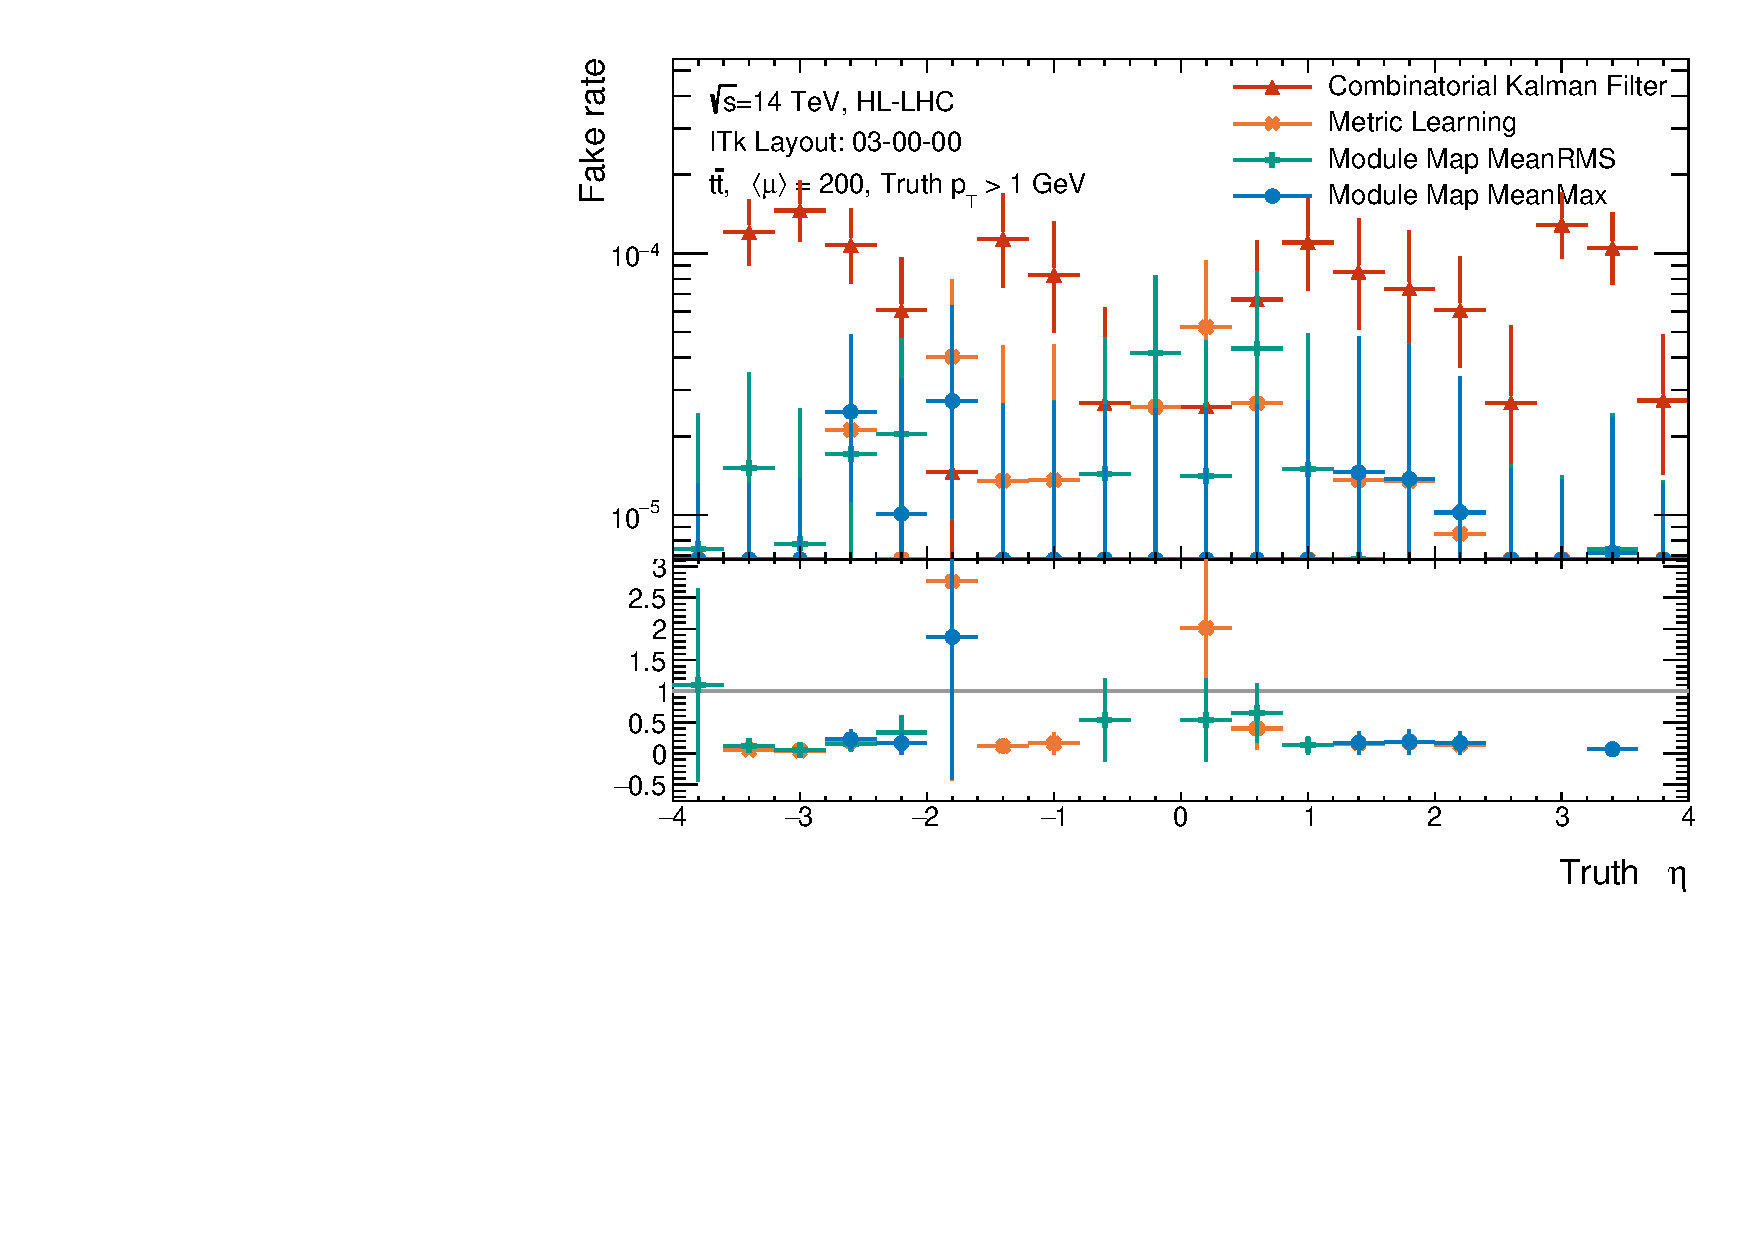
\includegraphics[width=\textwidth]{figures/ckf-gnn/FakeRate/fakerate_vs_eta.pdf}
    \caption{}
    \label{subfig:tracking-fake-eta}
\end{subfigure}
\begin{subfigure}[b]{0.6\textwidth}
    \centering
    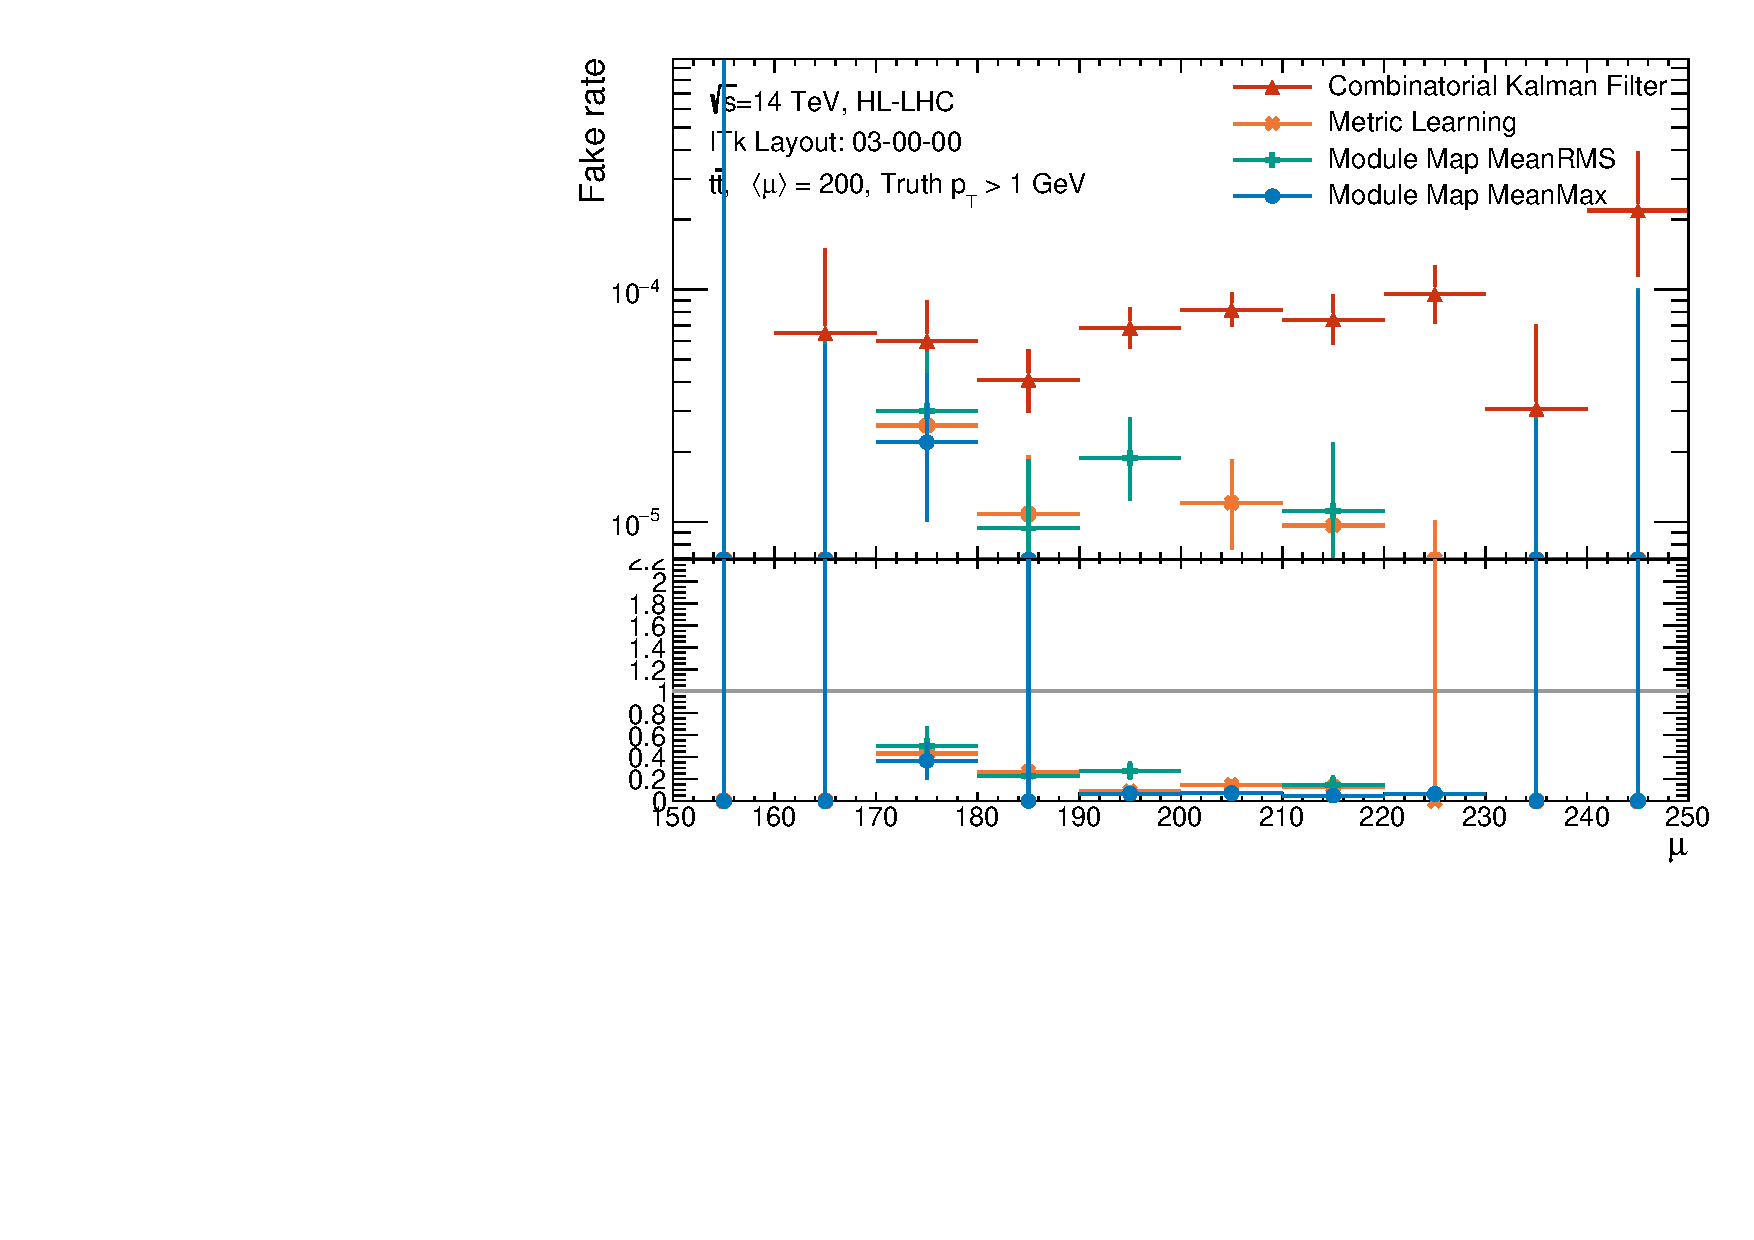
\includegraphics[width=\textwidth]{figures/ckf-gnn/FakeRate/fakerate_vs_mu.pdf}
    \caption{}
    \label{subfig:tracking-fake-mu}
\end{subfigure}
    \caption{The proportion of reconstructed tracks reconstructed by the GNN4ITk and CKF chains having matching probability less than 0.5 as a function of the track pseudorapidity $\eta$ (a) and the truth pile-up (b). The bottom plots show the ratio of the GNN-based curves to the CKF-based curve.}
    \label{fig:tracking-fake-eta-mu}
\end{figure}

Given the small number of fake tracks, it is difficult to examine their spatial distribution and variation with pile-up, the latter being of particular importance. 
This is due to the small number of $t\bar{t}$ events used in evaluation. 
Future work may address this problem with a larger test sample.

\newpage
\subsection{Parameter resolution}
\label{subsect:parameter-reso}

Track parameter resolution quantifies how well the reconstructed track candidate represents the underlying truth particle, and is thus an important aspect of tracking.
It is evaluated by comparing the parameters at the perigee surface extracted from the global $\chi^2$ fit discussed in section \ref{sect:chi2-fit} and the corresponding truth value using equation \ref{eq:track-fit:10}.
In MC simulation, the truth impact parameters are specified by the primary vertex position, and the truth kinematics the momentum at the vertex. 
The are generated along the particles and stored for tracking validation. 

\begin{figure}[h!]
\centering
\begin{subfigure}[b]{0.65\textwidth}
    \centering
    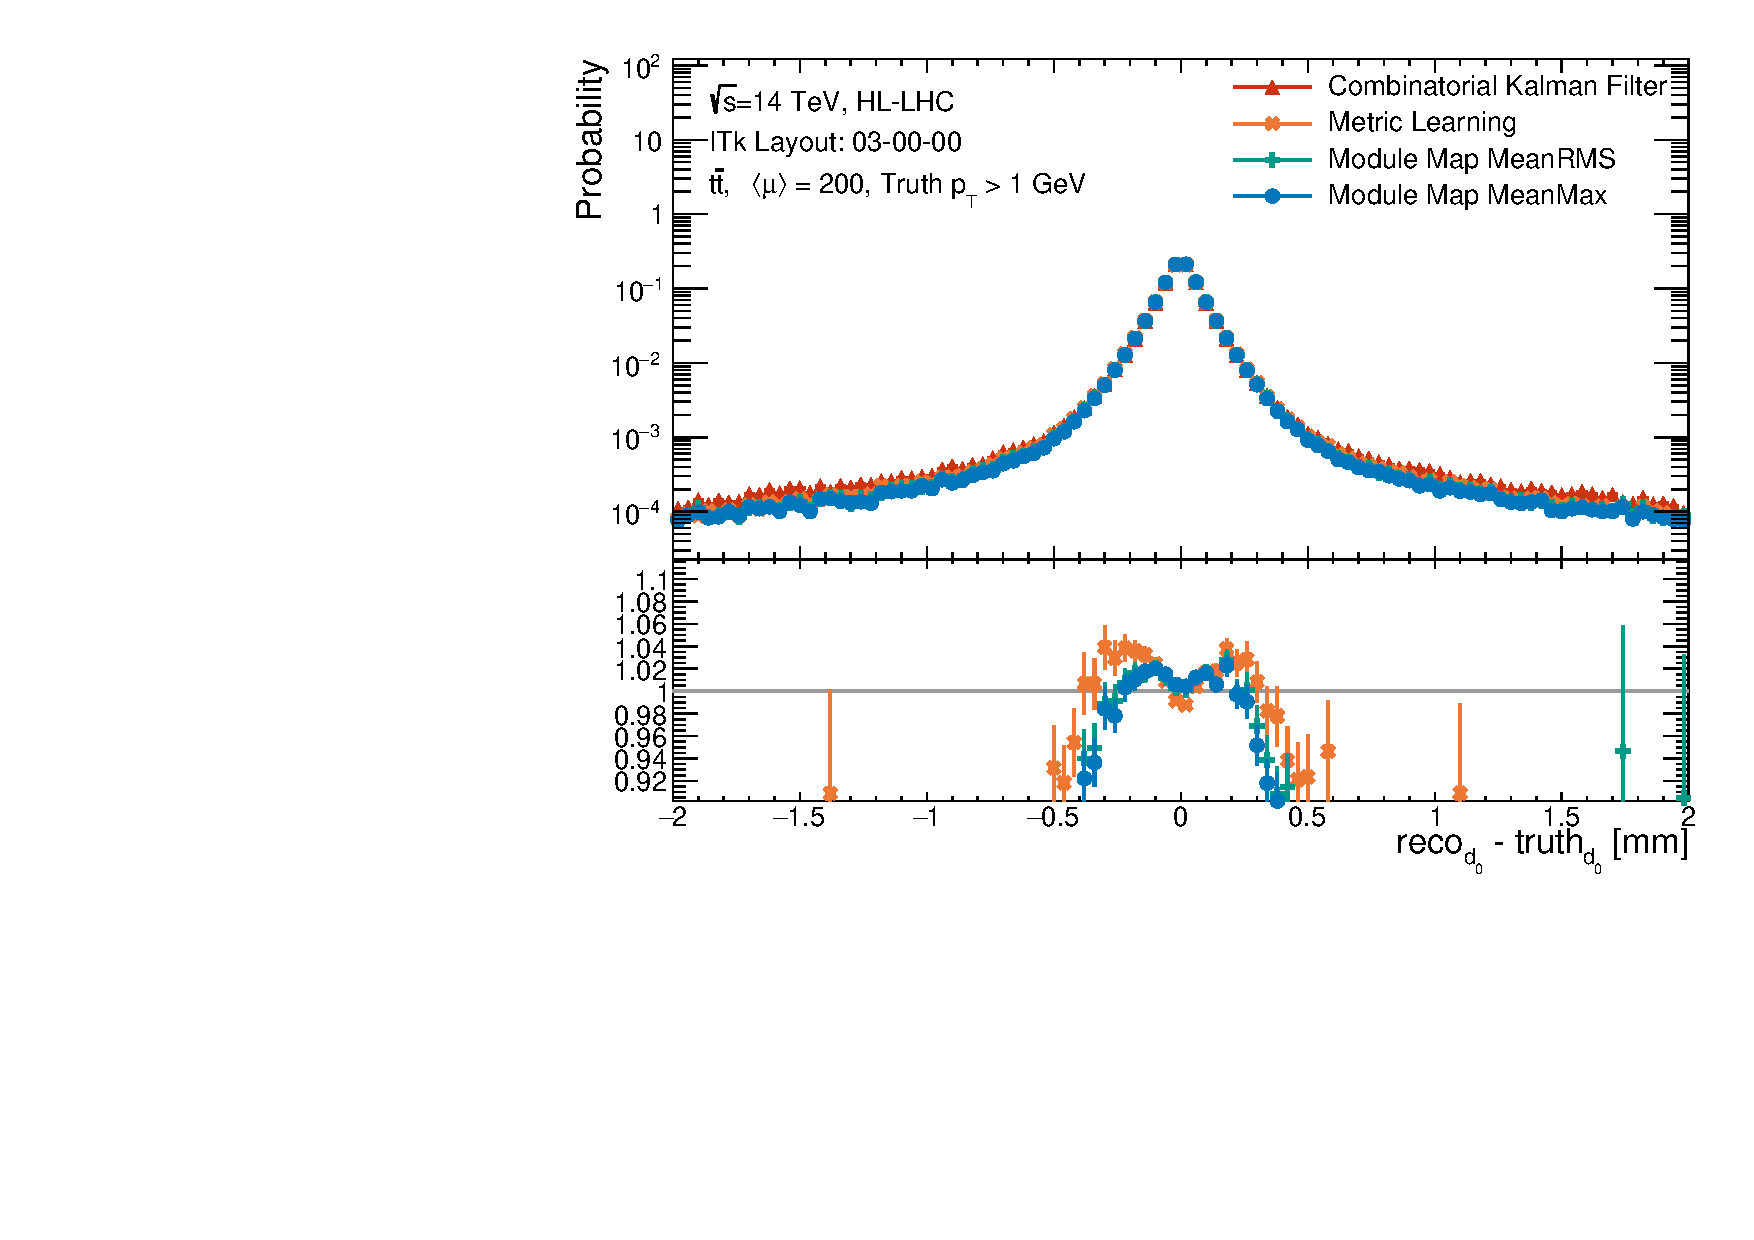
\includegraphics[width=\textwidth]{figures/ckf-gnn/Matched/Resolutions/Primary/res_d0.pdf}
    \caption{Transverse impact parameter resolution $\sigma(d_0)$}
    \label{subfig:res-d0}
\end{subfigure}
\begin{subfigure}[b]{0.65\textwidth}
    \centering
    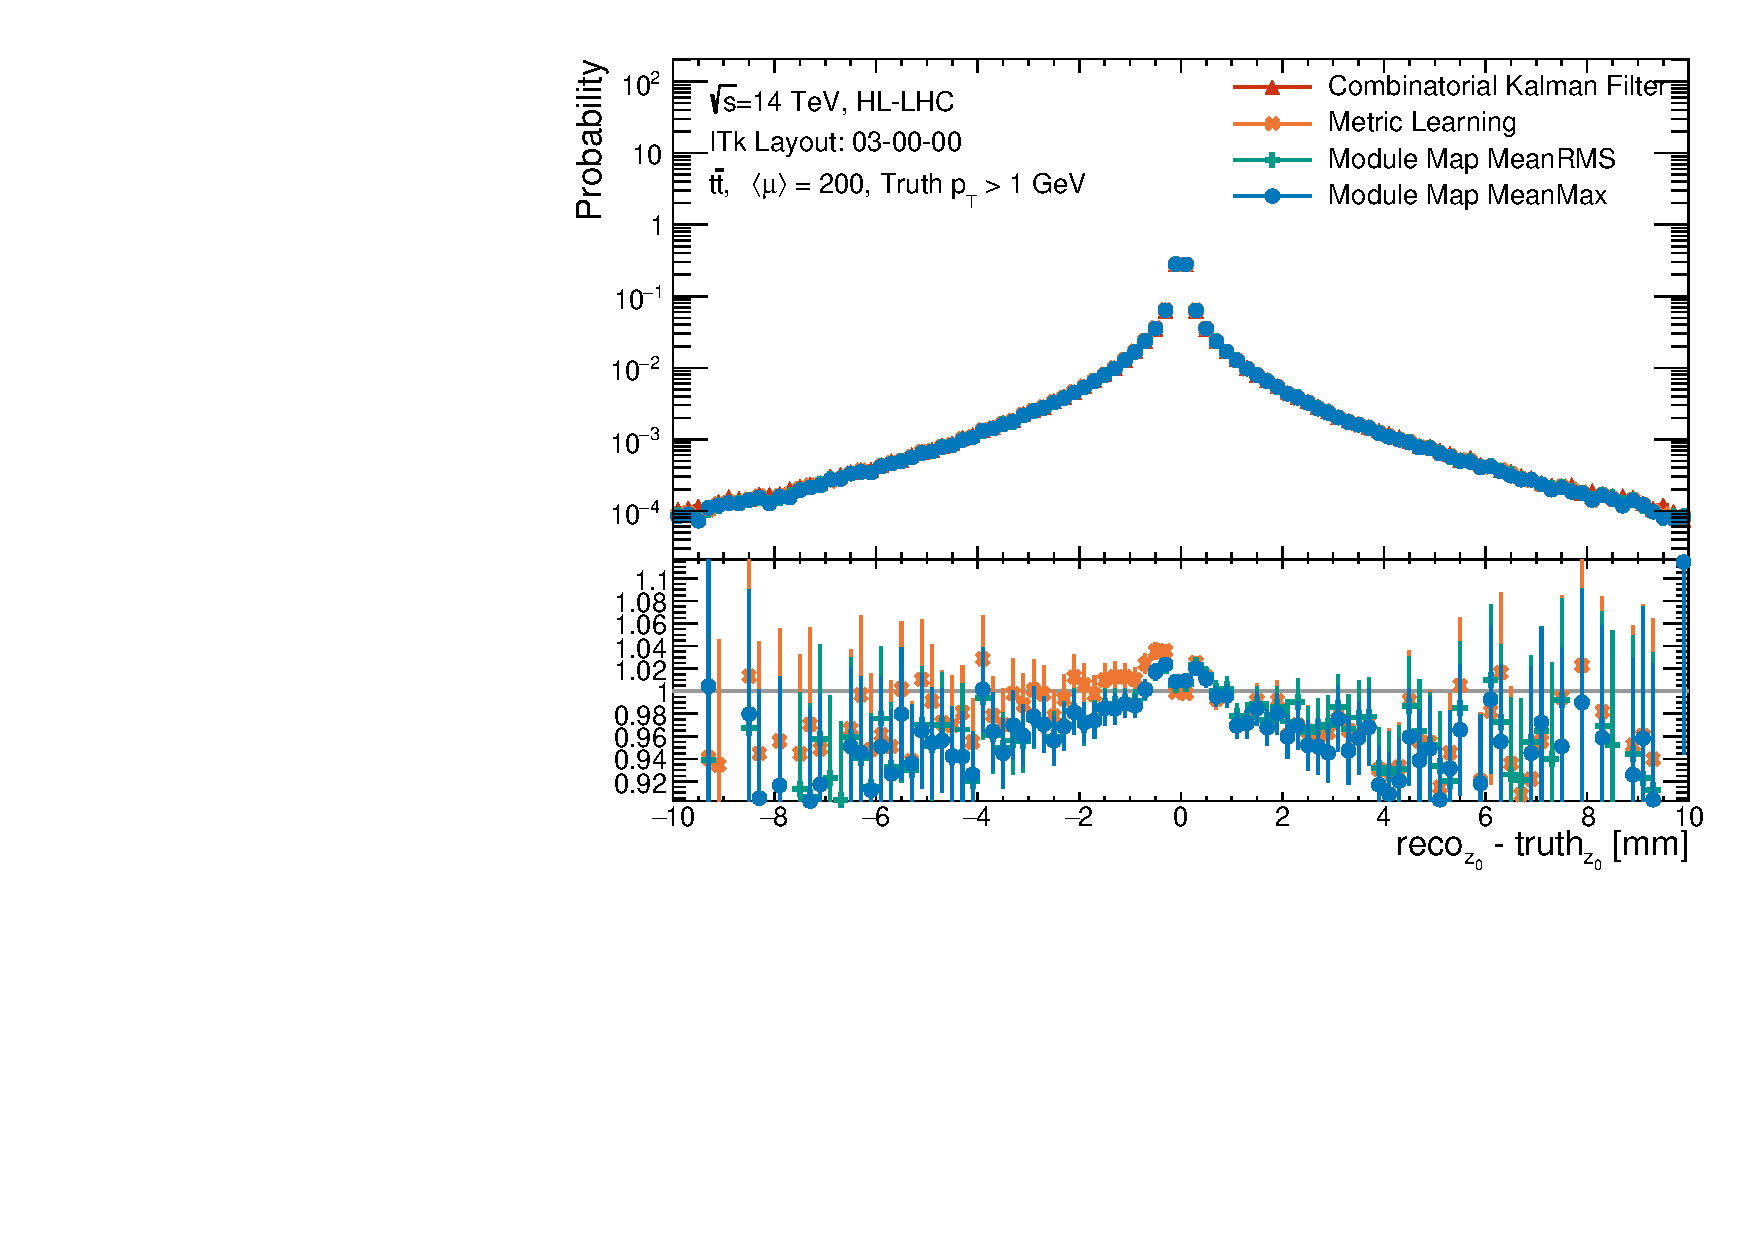
\includegraphics[width=\textwidth]{figures/ckf-gnn/Matched/Resolutions/Primary/res_z0.pdf}
    \caption{Longitudinal impact parameter resolution $\sigma(z_0)$}
    \label{subfig:res-z0}
\end{subfigure}
    \caption{Transverse (a) and longitudinal (b) impact parameter resolution shown as histograms of $\sigma(d_0)$ and $\sigma(z_0)$ respectively. Note that the resolution of parameter $x$ is inversely proportional to $\sigma(x)$.}
    \label{fig:res-d0-z0}
\end{figure}

The resolution of the longitudinal $(z_0)$ and transverse $(d_0)$ impact parameters of the track candidates produced by both the GNN- and CKF-based algorithms is shown in figure \ref{fig:res-d0-z0}. 
The vertical axis in these plots displays the number of matched track--particle pairs normalized to unity. 
All track builders show a spectrum peaking at $\sigma(d_0) = 0$ and $\sigma(z_0)=0$. 
In general, the GNN-based algorithms produce a larger proportion of tracks whose resolution concentrates around 0 for both impact parameters than does the CKF.
Despite having higher efficiency, i.e. reconstructing more particles, the GNN-based track candidates are less tail-heavy.
In other words, the excess tracks found by the GNN4ITk are overwhelmingly good-quality tracks accurately characterizing the impact parameters of the underlying particle.
The distributions from the two Module Map variants appear similar, while that of the Metric Learning variant is slightly more tail-heavy. 

% Impact parameter resolution is heavily determined by the innermost hit on the track candidate. 
The good resolution observed for the GNN-based algorithm can be explained by the efficiency in finding the hit on the innermost pixel layer, which provides a strong constraint on the impact parameters. 
Figure \ref{fig:n-innermost-pix} shows the number innermost pixel hits as a function of track pseudorapidity.
The Module Map variants build tracks with the same average number of innermost pixel hits as does the CKF, with tracks in the barrel region having $\expval{N_{pix,innermost}}=1$.
The Metric Learning variant is slightly less hit-efficient in the barrel, which would explain its lower resolution.

\begin{figure}[h!]
    \centering
    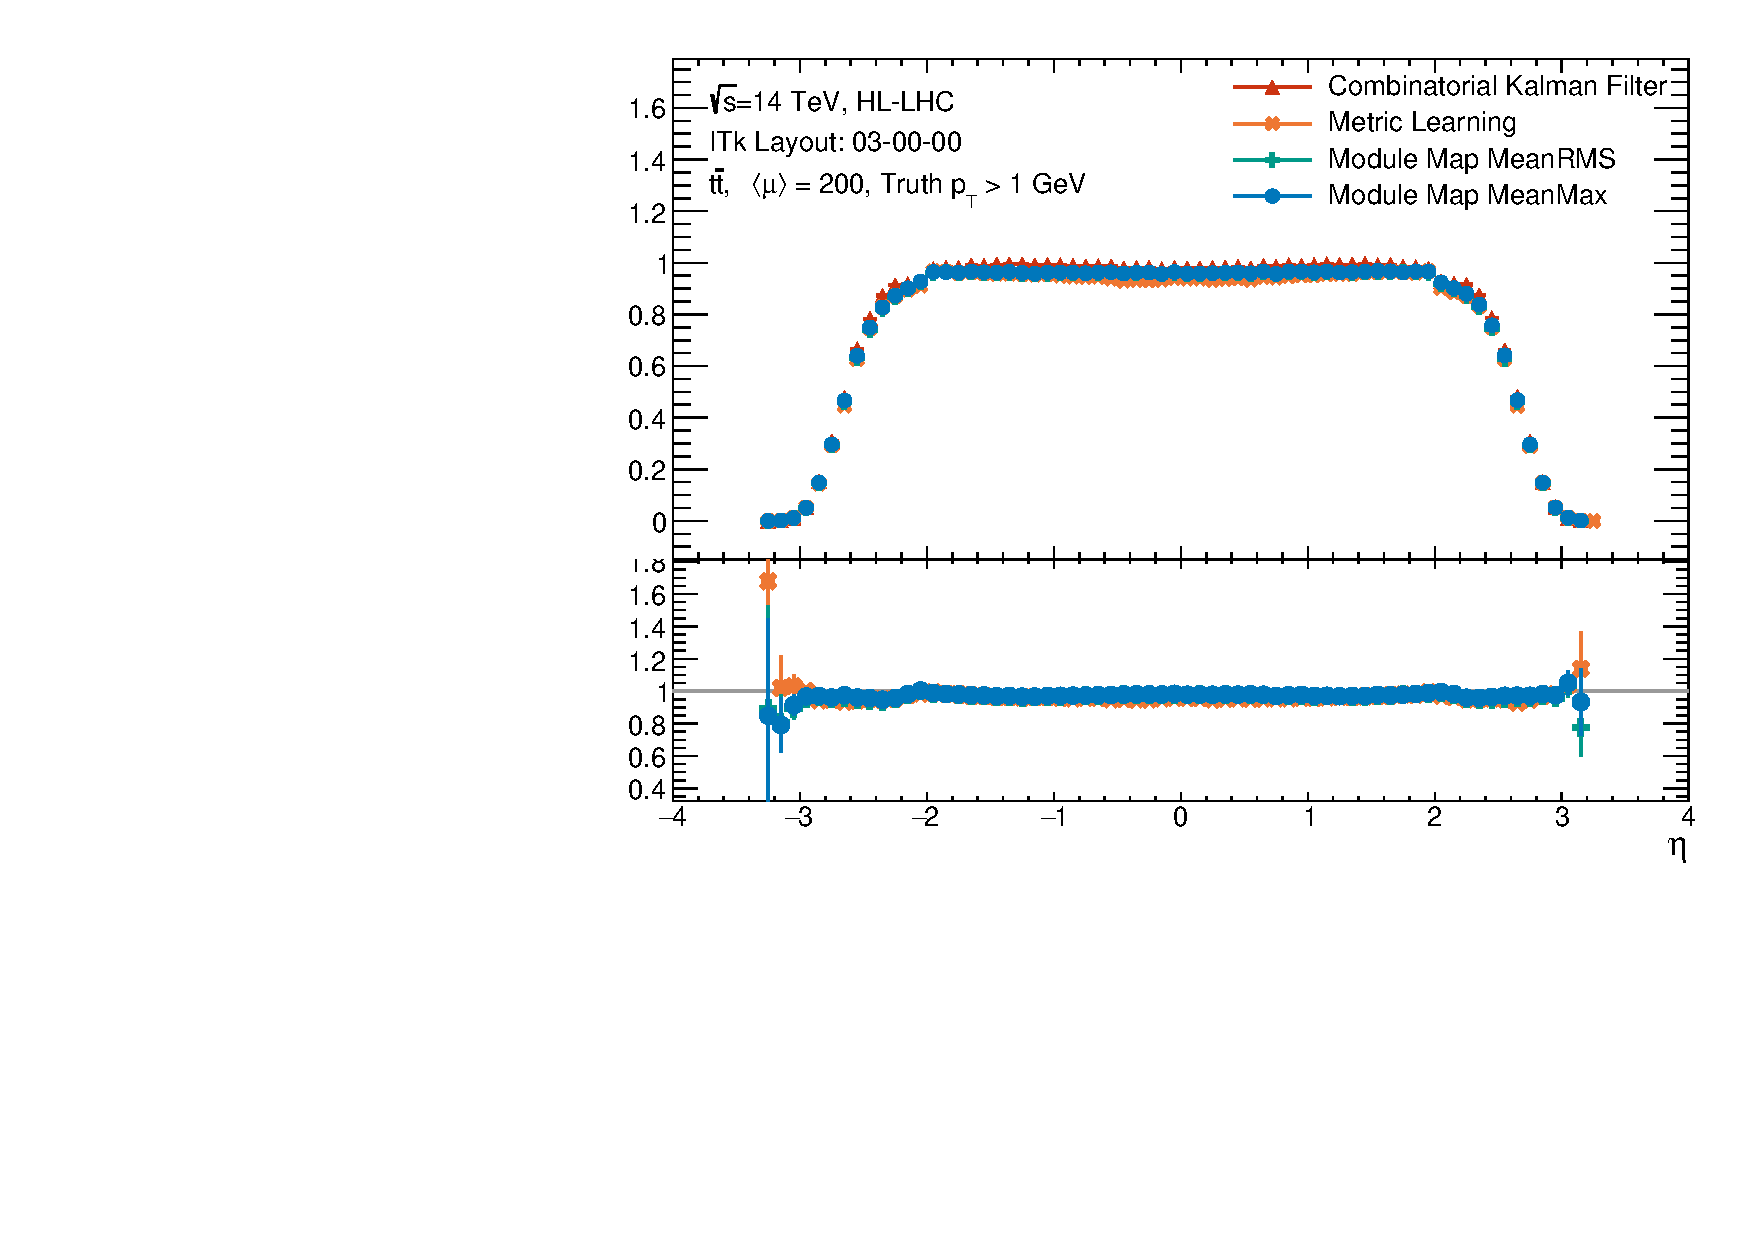
\includegraphics[width=0.65\textwidth]{figures/ckf-gnn/HitsOnTracks/nInnerMostPixelHits_vs_eta.pdf}
    \caption{The number of hits from the inner most pixel layer as a function of reconstructed pseudorapidity $\eta$.}
    \label{fig:n-innermost-pix}
\end{figure}

\begin{figure}[h!]
\centering
    \centering
    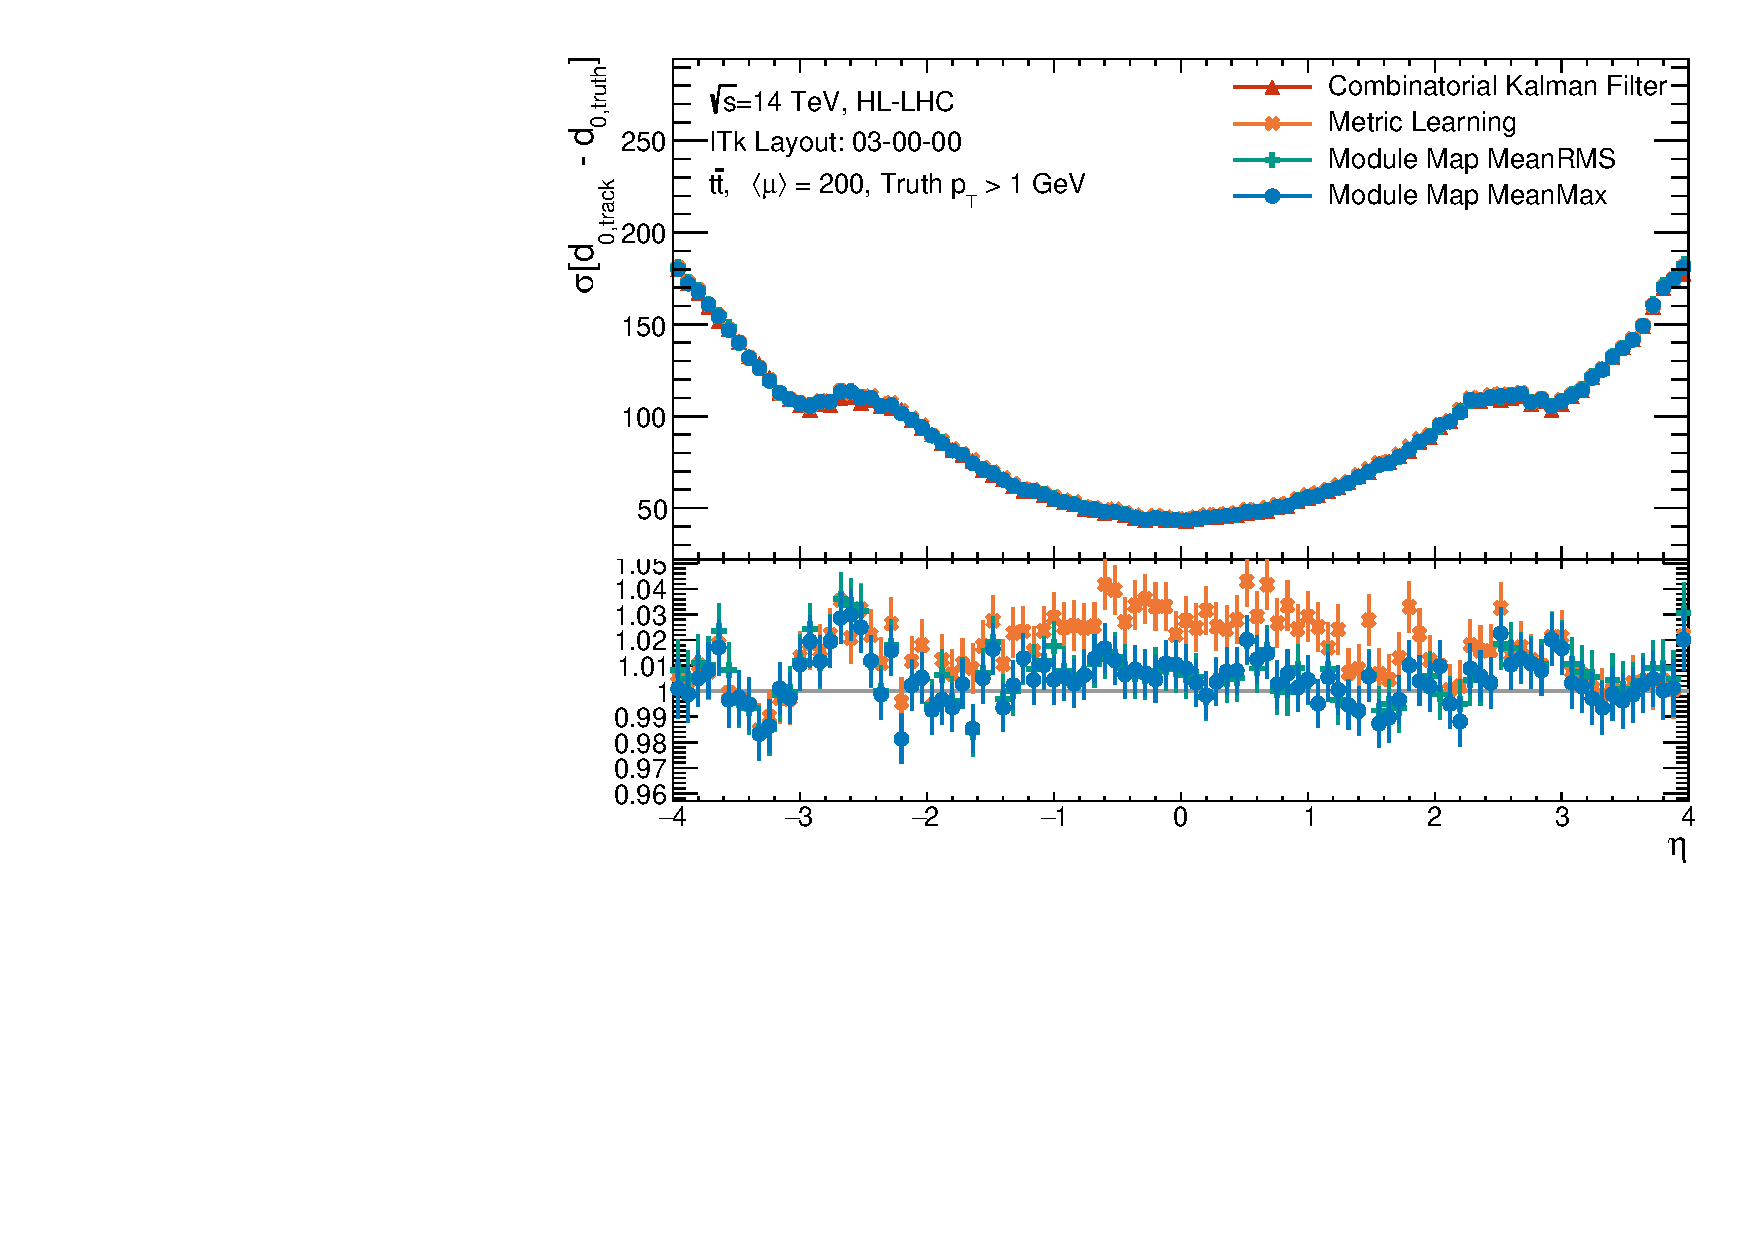
\includegraphics[width=0.65\textwidth]{figures/ckf-gnn/Matched/Resolutions/Primary/resolution_vs_eta_d0.pdf}
    \caption{  Transverse impact parameter resolution $\sigma(d_0)$ of as a function of truth $\eta$, evaluated on tracks reconstructed by the GNN4ITk and the CKF chains. The bottom plots show the ratio of the GNN-based curves to the CKF-based curve. }
    \label{fig:res-vs-eta-d0}
\end{figure}

Another measure of resolution is the RMS of the core of the distribution of the difference between the reconstructed and true values of the parameter. 
Figures \ref{fig:res-vs-eta-d0} and \ref{fig:res-vs-eta-z0} respectively show the RMS of the $(d_{0,reco} - d_{0,truth})$ distribution and the the $(z_{0,track} - z_{0,truth})$ distribution, measured in $\mu$m, as a function of $\eta$. 
Over the entire $\eta$ range, the resolution of the Module Map variants is in good agreement with that of the CKF, while that of the Metric Learning is slightly degraded in the barrel region. 
Here we can clearly observe the correlation between the number of innermost pixel hits and the impact parameter resolution, as the degradation occurs where the former quantity is the most deficient among the the Metric Learning track candidates.

\begin{figure}[h!]
\centering
    \centering
    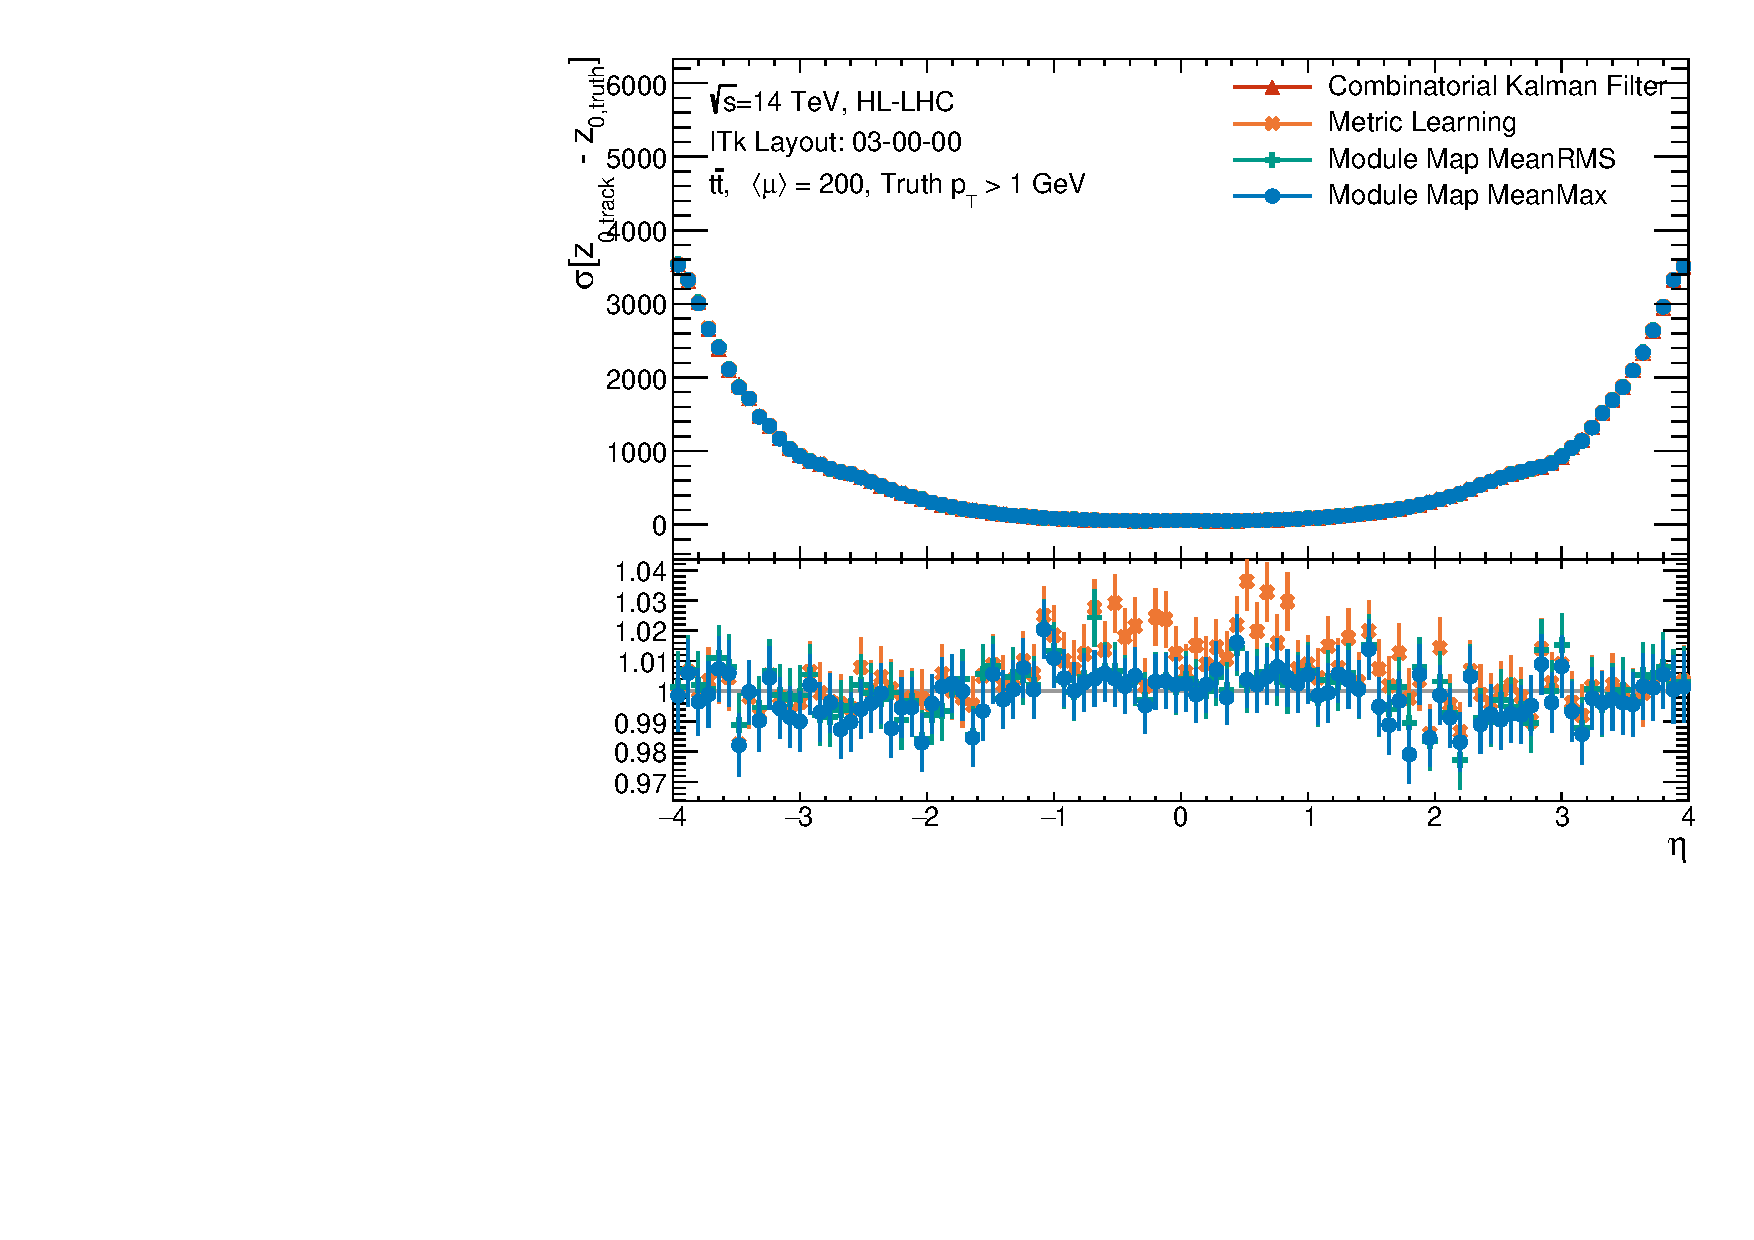
\includegraphics[width=0.65\textwidth]{figures/ckf-gnn/Matched/Resolutions/Primary/resolution_vs_eta_z0.pdf}
    \caption{Longitudinal impact parameter resolution $\sigma(z_0)$ of as a function of truth $\eta$, evaluated on tracks reconstructed by the GNN4ITk and the CKF chains. The bottom plots show the ratio of the GNN-based curves to the CKF-based curve.}
    \label{fig:res-vs-eta-z0}
\end{figure}

\newpage
The transverse momentum resolution as a histogram is shown in figure \ref{subfig:res-pt-hist} and as a function of $\eta$ in figure \ref{subfig:res-pt-eta}.
Unlike the other parameters' resolution, the dimensionless transverse momentum resolution is computed as $$
\sigma(\pT) = p_{T,truth}  \times \left ( \frac{q}{p_{T, reco}} - \frac{q}{p_{T, truth}} \right).$$
While other track parameters are directly obtained from the $\chi^2$ fit, the transverse momentum is derived from the total momentum $p$ and the azimuthal angle $\theta$ in the ATLAS parametrization (equation \eqref{eq:tracking-performance:1}). 
There is no straightforward relationship between its resolution and elements of the global fit.
However, given that it is derived from fit parameter $q/p$, whose uncertainty is driven by material interaction, one expects lower \pT resolution with more detector material encountered on the trajectory.
This effect is observed on figure \ref{subfig:res-pt-eta},  viewed in tandem with figure \ref{subfig:itk-rad-len}, which shows the material budget traversed by a straight track in radiation length as a function of the particle's pseudorapidity.
The total radiation length increases generally with $\eta$, so the closer to the beamline is the particle, the more its energy--and thus momentum--is eroded, weakening the constraints on \pT. 
In consequence, the \pT resolution decreases monotonically with $\eta$.

\begin{figure}[h!]
\centering
\begin{subfigure}[b]{0.65\textwidth}
    \centering
    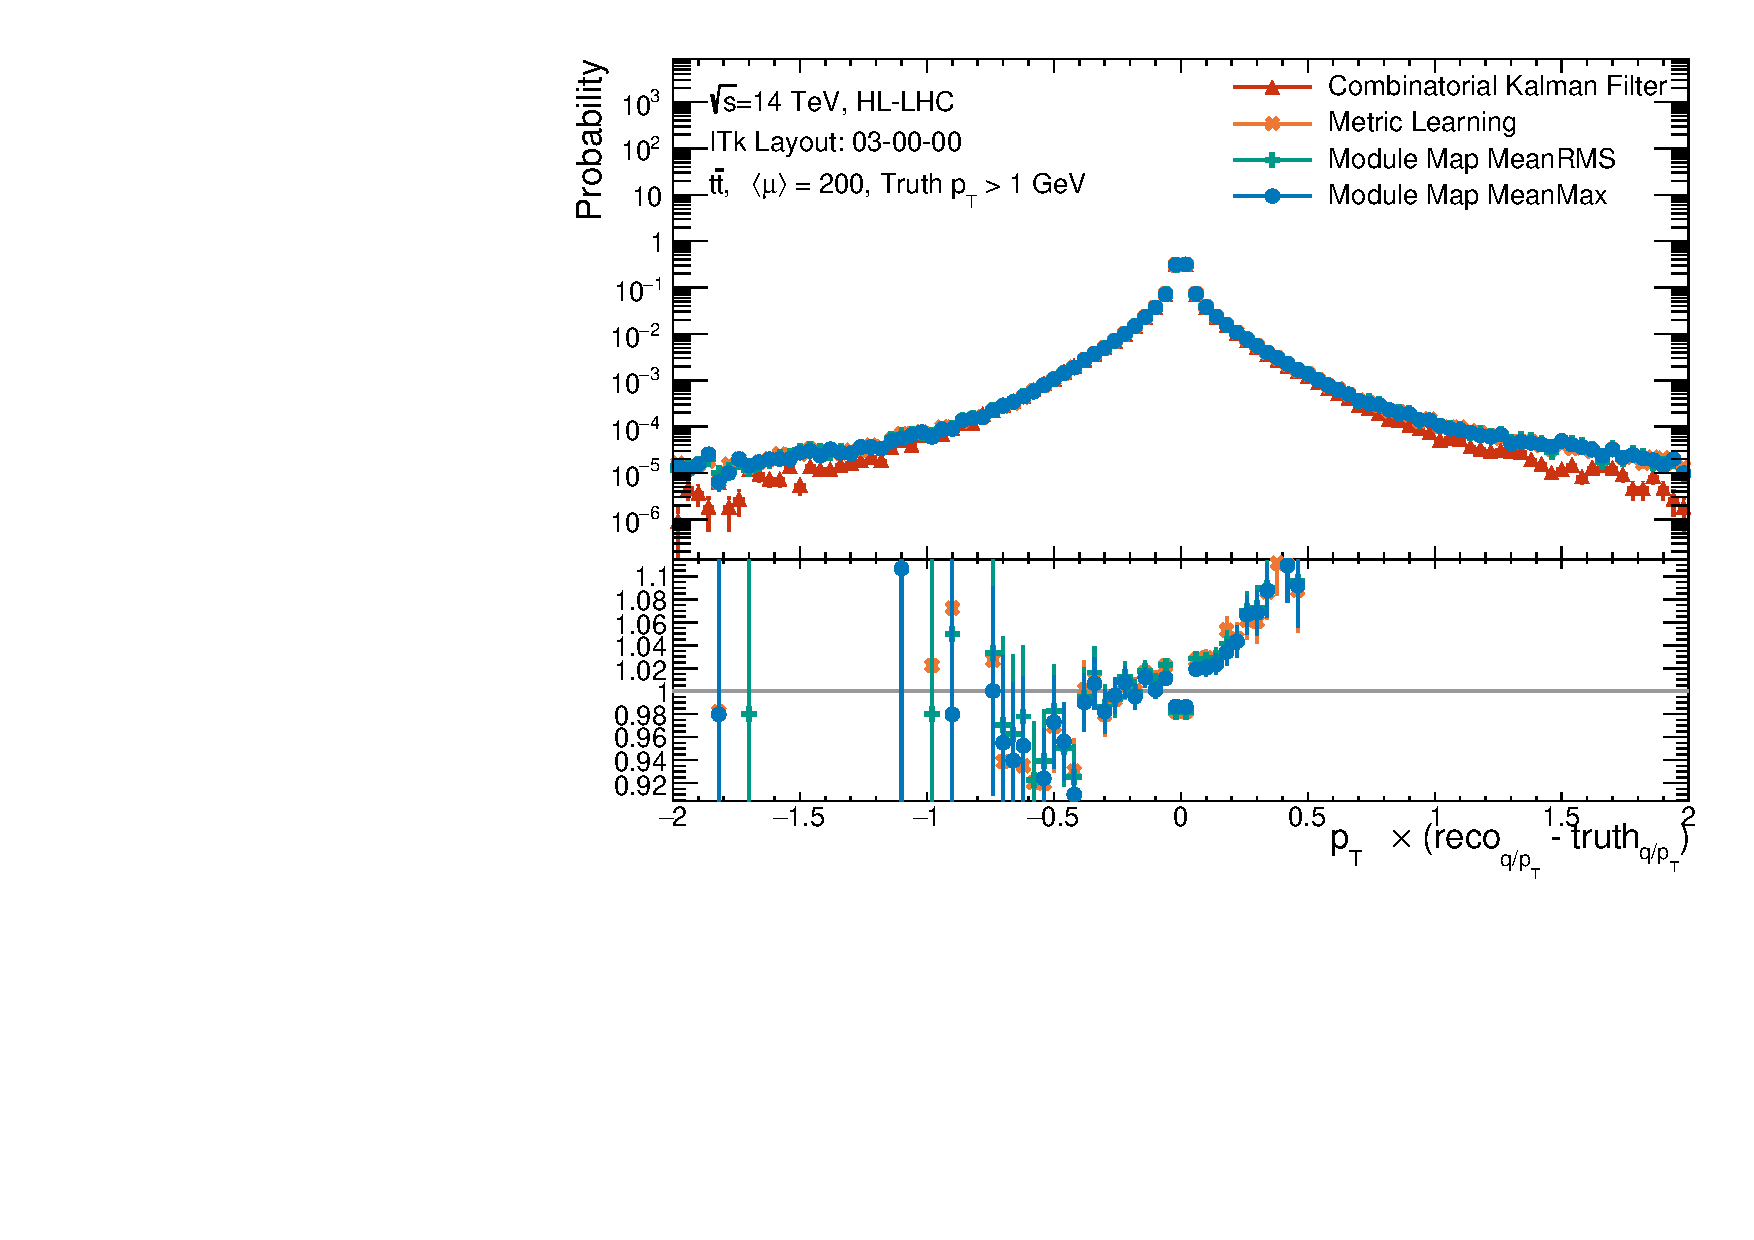
\includegraphics[width=\textwidth]{figures/ckf-gnn/Matched/Resolutions/Primary/res_ptqopt.pdf}
    \caption{Transverse momentum resolution $\pT  \times \left ( \frac{q}{p_{T, reco}} - \frac{q}{p_{T, truth}} \right)$}
    \label{subfig:res-pt-hist}
\end{subfigure}
\begin{subfigure}[b]{0.65\textwidth}
    \centering
    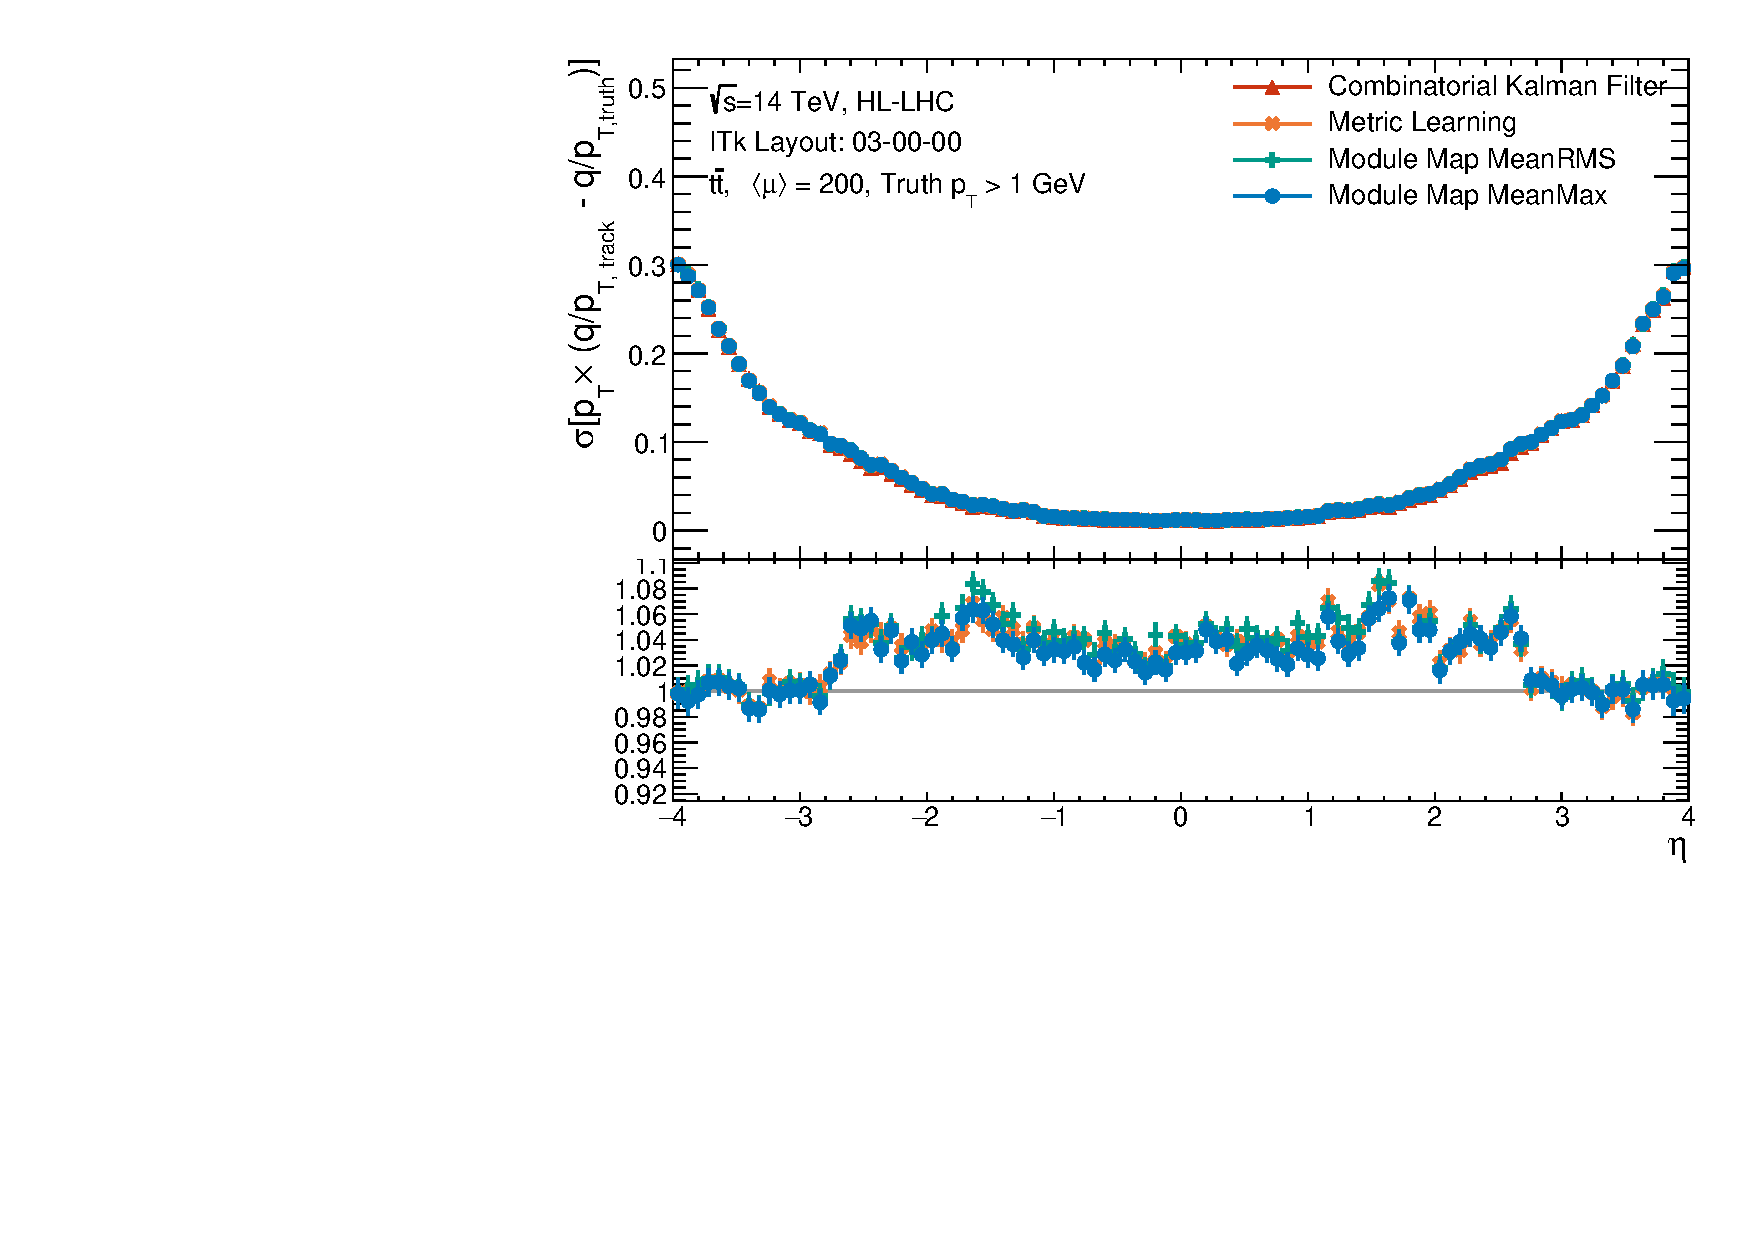
\includegraphics[width=\textwidth]{figures/ckf-gnn/Matched/Resolutions/Primary/resolution_vs_eta_ptqopt.pdf}
    \caption{Transverse momentum resolution $\pT \times \left ( \frac{q}{p_{T, reco}} - \frac{q}{p_{T, truth}} \right)$ as a function of $\eta$}
    \label{subfig:res-pt-eta}
\end{subfigure}
    \caption{Transverse momentum resolution shown as a histogram of $\sigma(\pT)$ (a) and a function of the truth pseudorapidity $\eta$ (b). }
    \label{fig:res-pt}
\end{figure}

The transverse momentum is proportional to the radius of the curved trajectory, which in turn is geometrically constrained by the hits found between the outermost hits of the track candidate\footnote{Intuitively, imagine fitting a circle passing through two outermost points. If no intermediate points exists, any of infinitely many possible circles is equally likely, hence null constraint. If an intermediate measurement exists with some measurement error, the closer a circle passes by the points, the more likely hit is. More intermediate measurements provide better constraining power, hence better resolution.}.
Therefore, the \pT resolution generally improves with the number of measurements and degrades with the number of holes of the track candidate. 
In light of this principle, the difference in \pT resolution between the GNN4ITk and the CKF may be elucidated.
On figure \ref{subfig:res-pt-eta}, the observed \pT resolution of the GNN4ITk is similar to that of the CKF in the all-pixel region, for $\abs{\eta}>2.6$.
Both algorithms find relatively long tracks in this region, having on average 13--14 hits, shown in figure \ref{subfig:n-pix-hits}. 
Track candidates from the GNN4ITk are slightly shorter than those from the CKF.
However, these the former contains on average fewer holes, as seen on figure \ref{subfig:n-pix-holes}. 
In other words, pixel-only GNN-tracks are shorter, but skip fewer layers than do the CKF counterparts.
Though not simply quantifiable, these factors have opposite impacts on the \pT resolution and likely yield similar performance in this region in effect.

On the other hand, in the barrel $(\abs{\eta}<2)$ and transition regions $(2<\abs{\eta}<2.6)$, the \pT resolution of all GNN-based variants is lower than that of the CKF.
The RMS width of the $\sigma(\pT)$-distribution from the GNN4ITk is at worst $8\%$ larger than from CKF.
In this region, the GNN-based tracks contain fewer clusters and more holes than the CKF-based tracks.
The gap is particularly pronounced in the strip detector, due to the presence of single clusters. 
In the barrel, despite the same average number of pixel clusters and negligible numbers of pixel holes, the GNN4ITk finds about $90\%$ the average number of strip hits found by the CKF, and leaves up to 5 times the number of holes left by the latter.
In the transition region, this trend repeats.
The combination of cluster deficiency and enrichment of holes explains the degraded \pT resolution in this region.
In general, the GNN, being trained on incomplete data, performs worse than the CKF does in the strip detector. 
In addition, the relaxed track selection cuts in $\abs{\eta}<2.6$--range allow short and layer-skipping GNN tracks to pass through, contributing to their increased abundance.
This is the trade-off we make in exchange for better efficiency.

\begin{figure}[h!]
\centering
\begin{subfigure}[b]{0.49\textwidth}
    \centering
    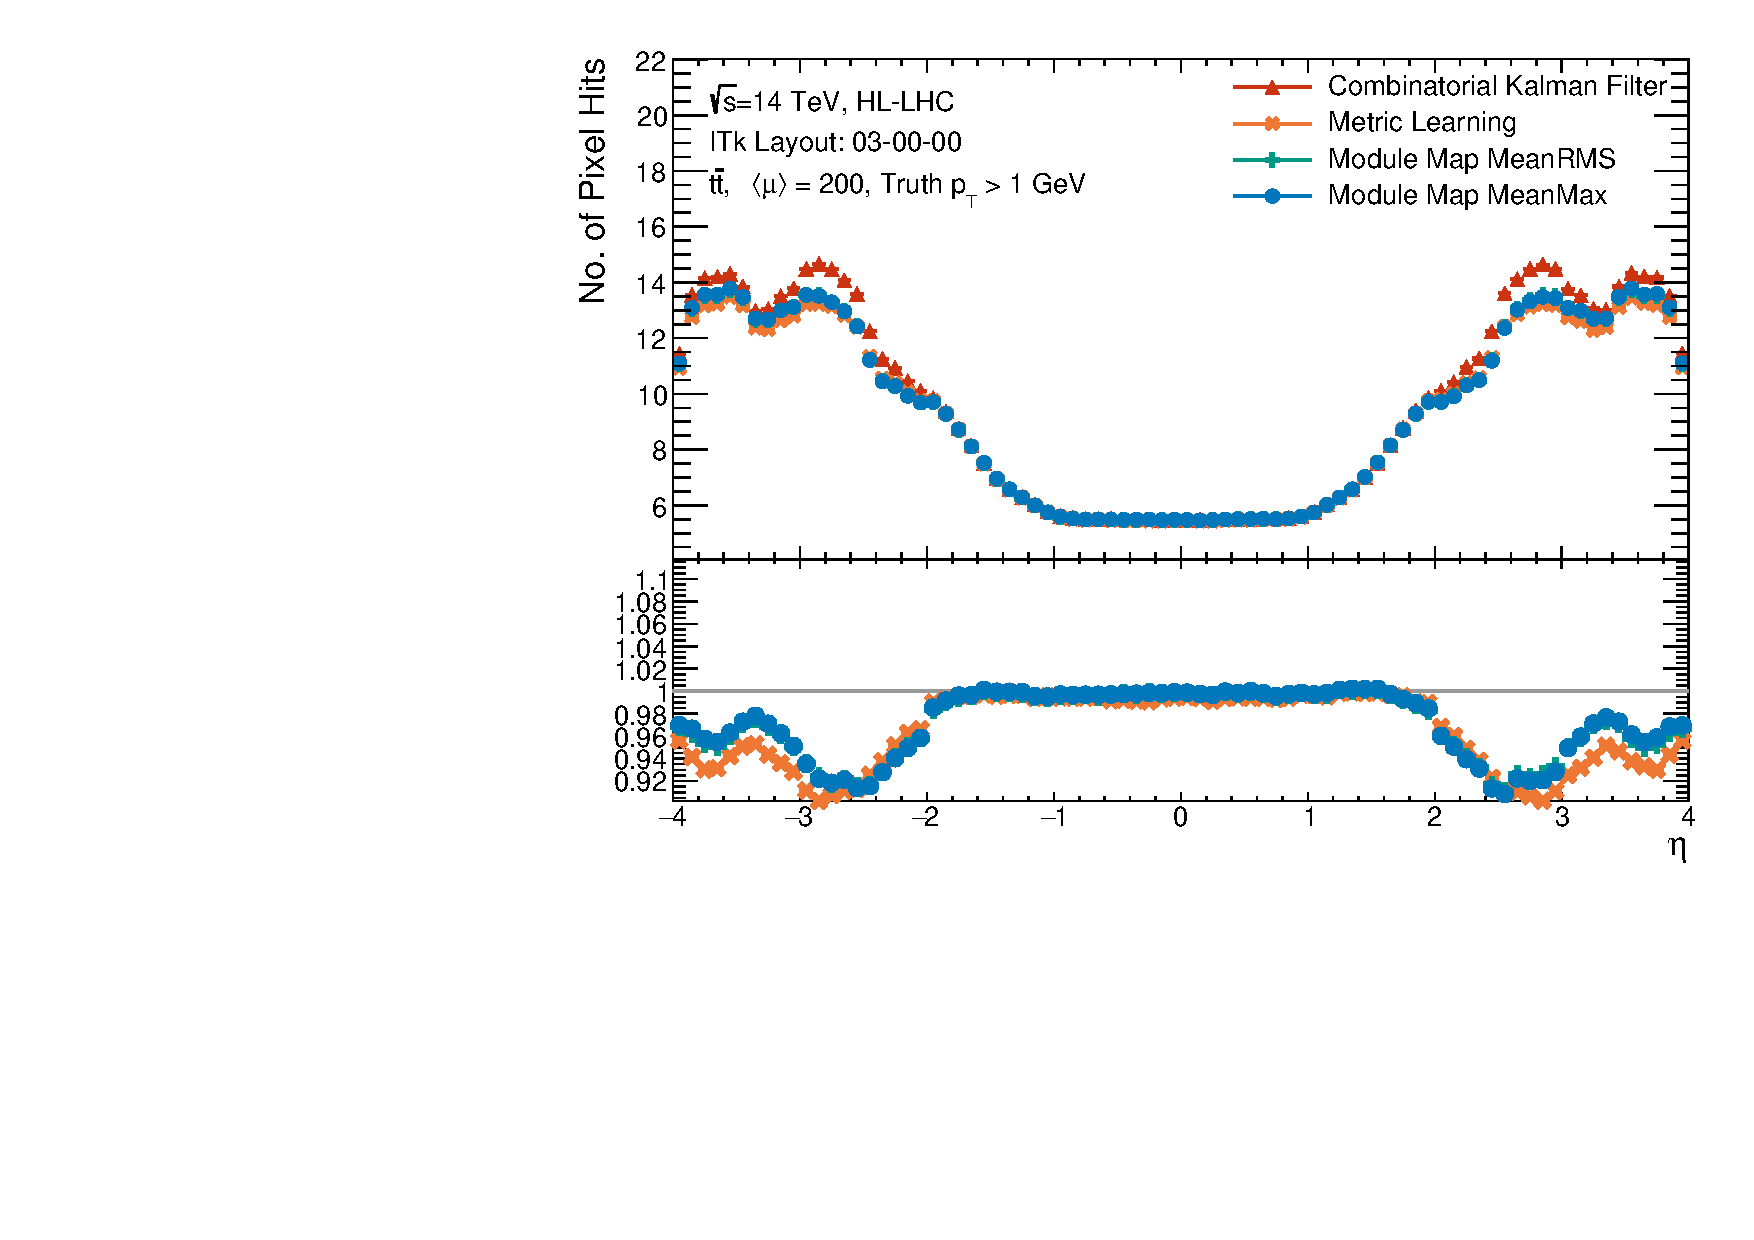
\includegraphics[width=\textwidth]{figures/ckf-gnn/HitsOnTracks/nPixelHits_vs_eta.pdf}
    \caption{Average number of pixel clusters on selected track candidates.}
    \label{subfig:n-pix-hits}
\end{subfigure}
\begin{subfigure}[b]{0.49\textwidth}
    \centering
    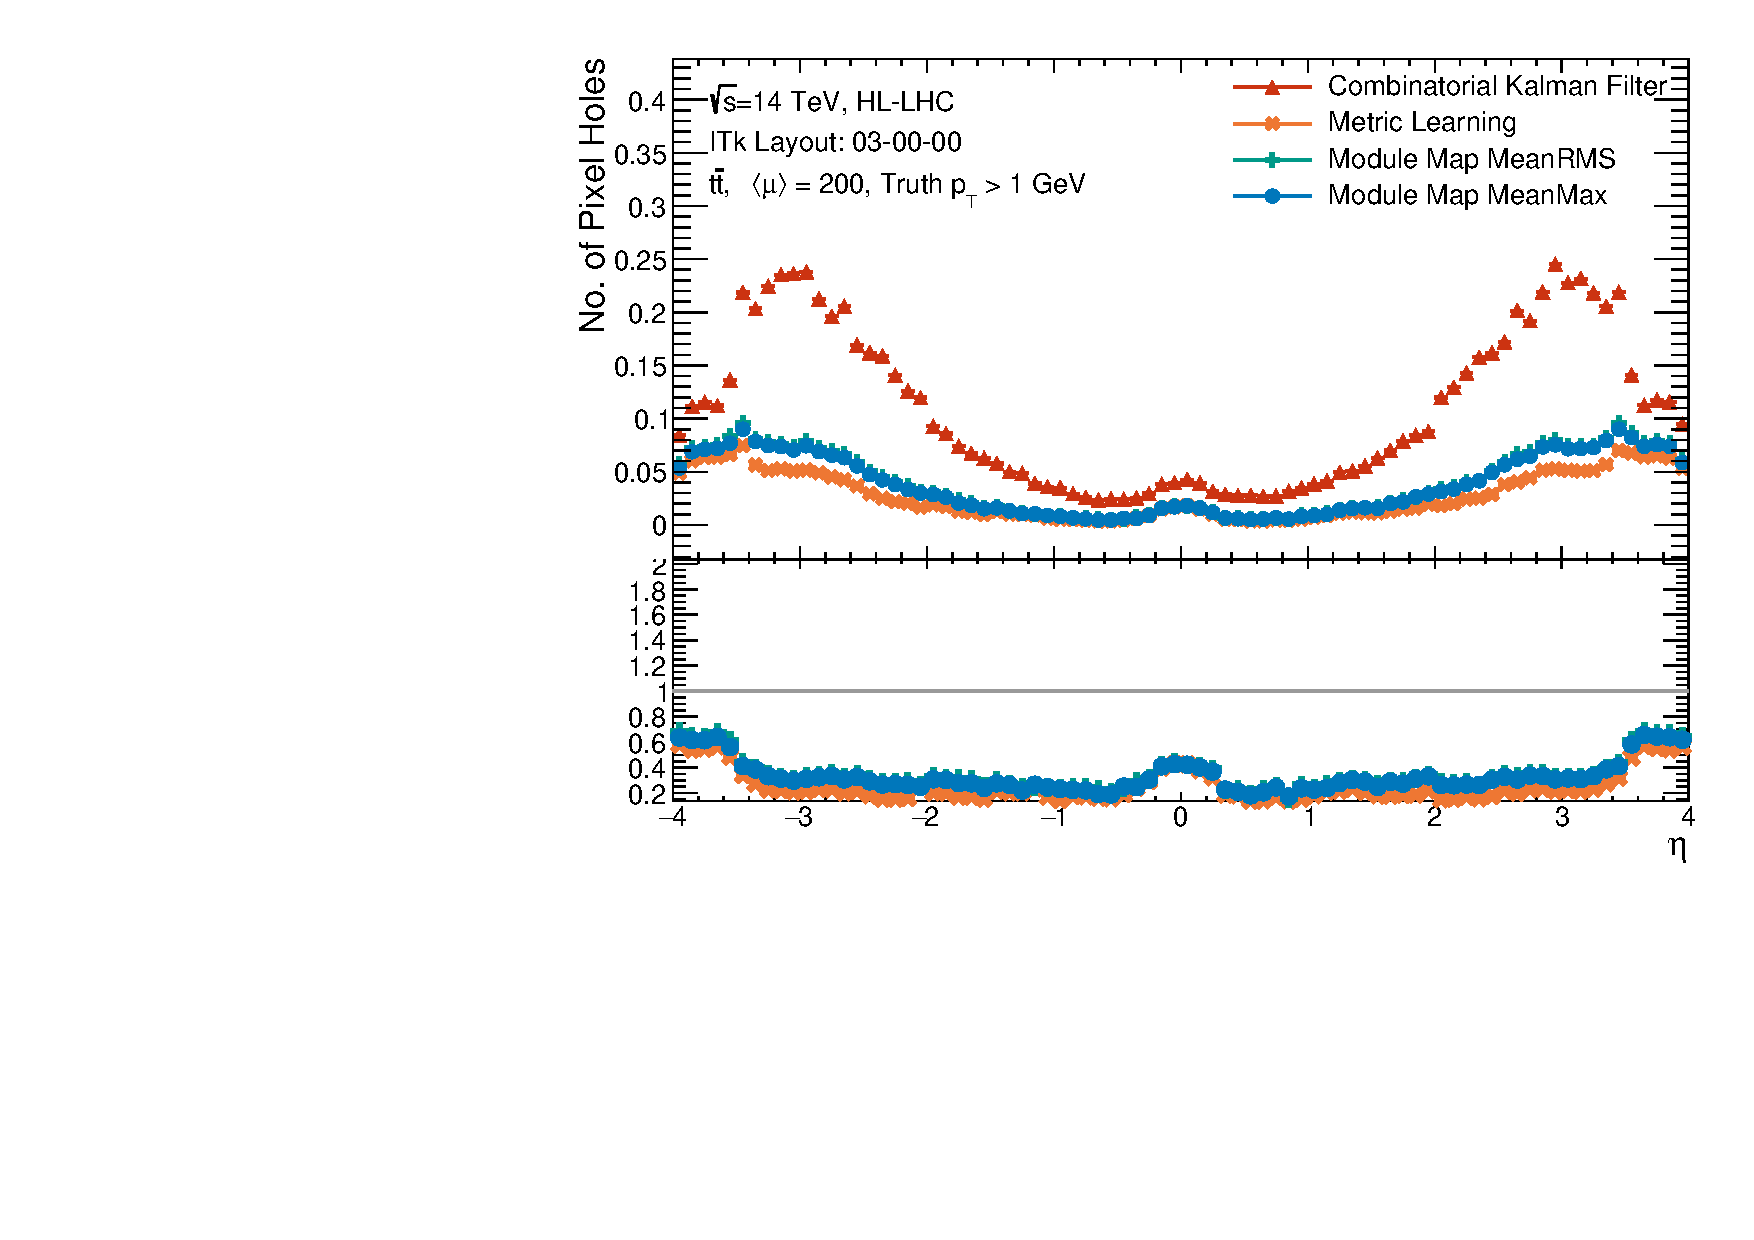
\includegraphics[width=\textwidth]{figures/ckf-gnn/HitsOnTracks/nPixelHoles_vs_eta.pdf}
    \caption{Average number of pixel holes on selected track candidates.}
    \label{subfig:n-pix-holes}
\end{subfigure}
\begin{subfigure}[b]{0.49\textwidth}
    \centering
    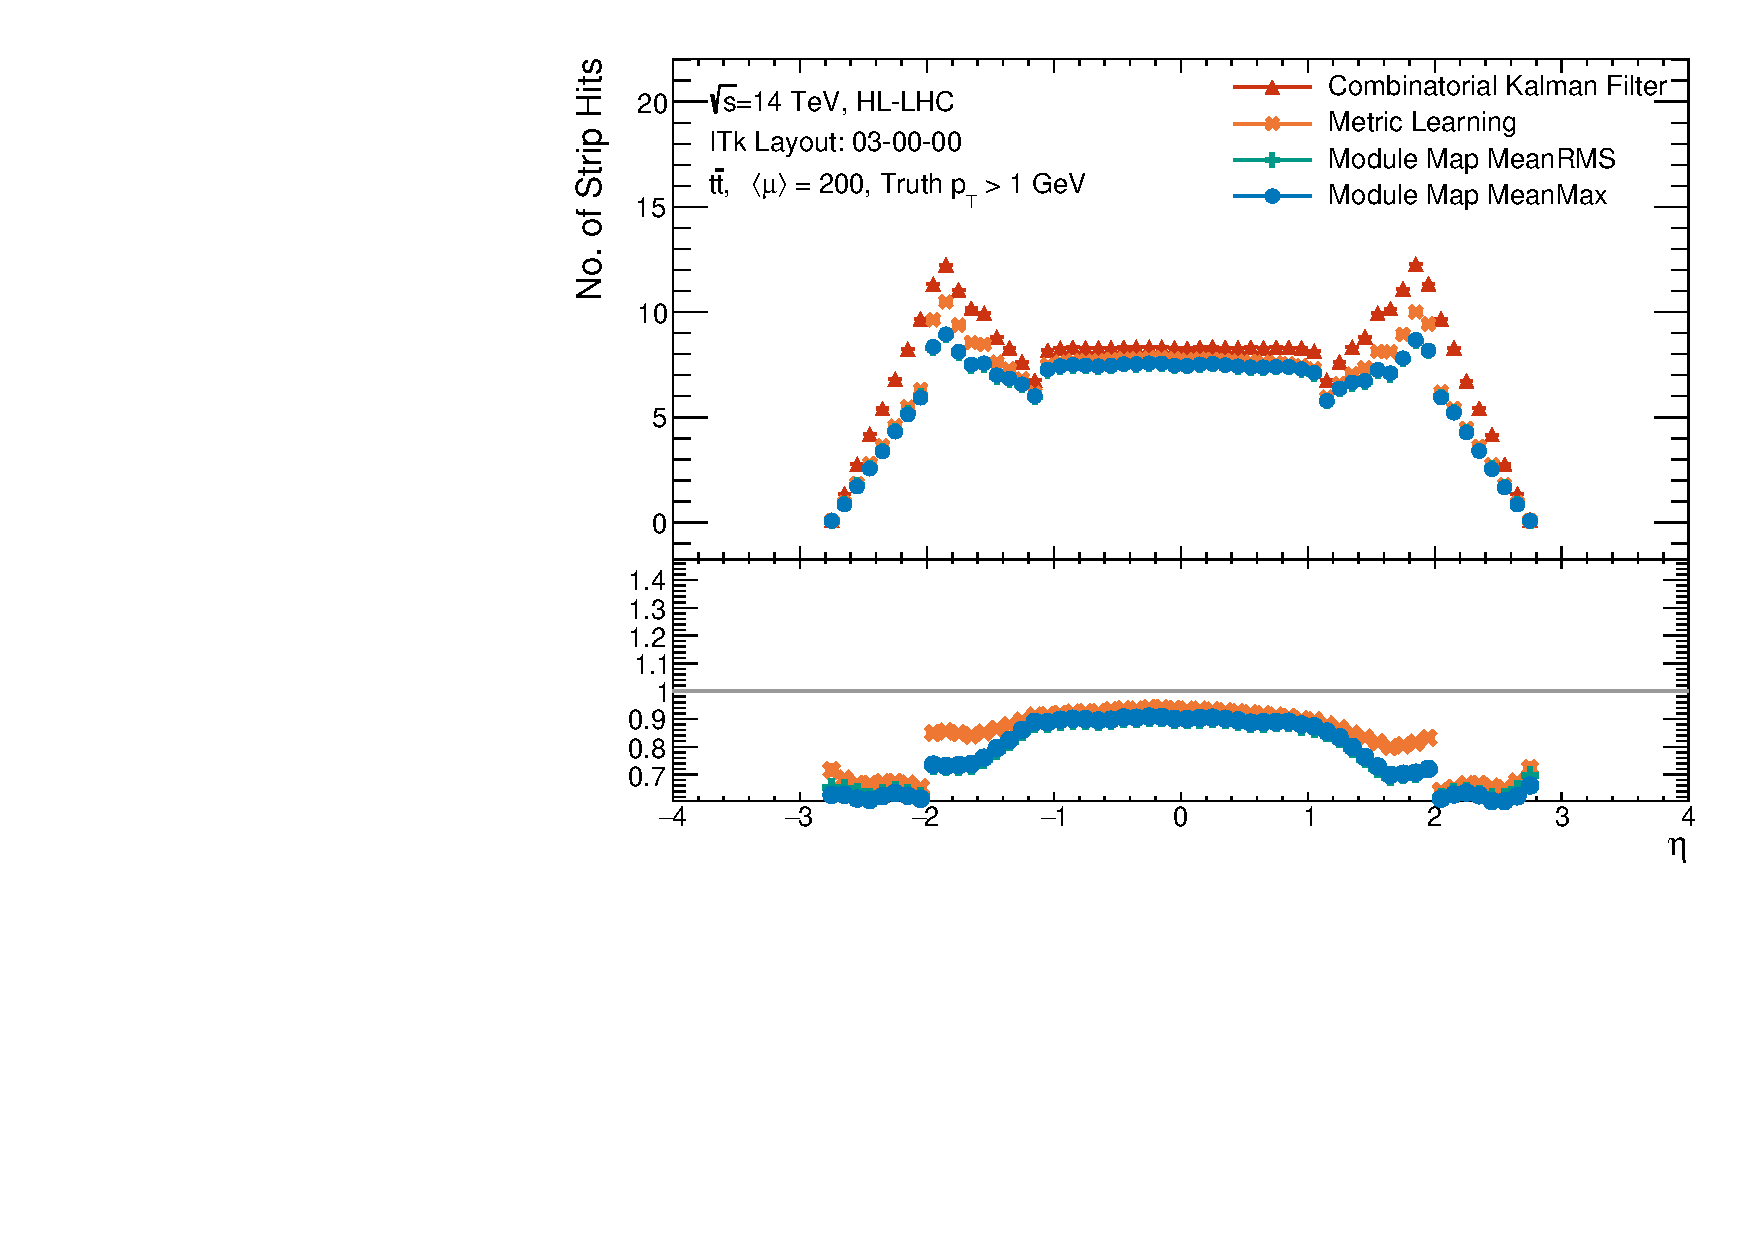
\includegraphics[width=\textwidth]{figures/ckf-gnn/HitsOnTracks/nSCTHits_vs_eta.pdf}
    \caption{Average number of strip clusters on selected track candidates}
    \label{subfig:n-strip-hits}
\end{subfigure}
\begin{subfigure}[b]{0.49\textwidth}
    \centering
    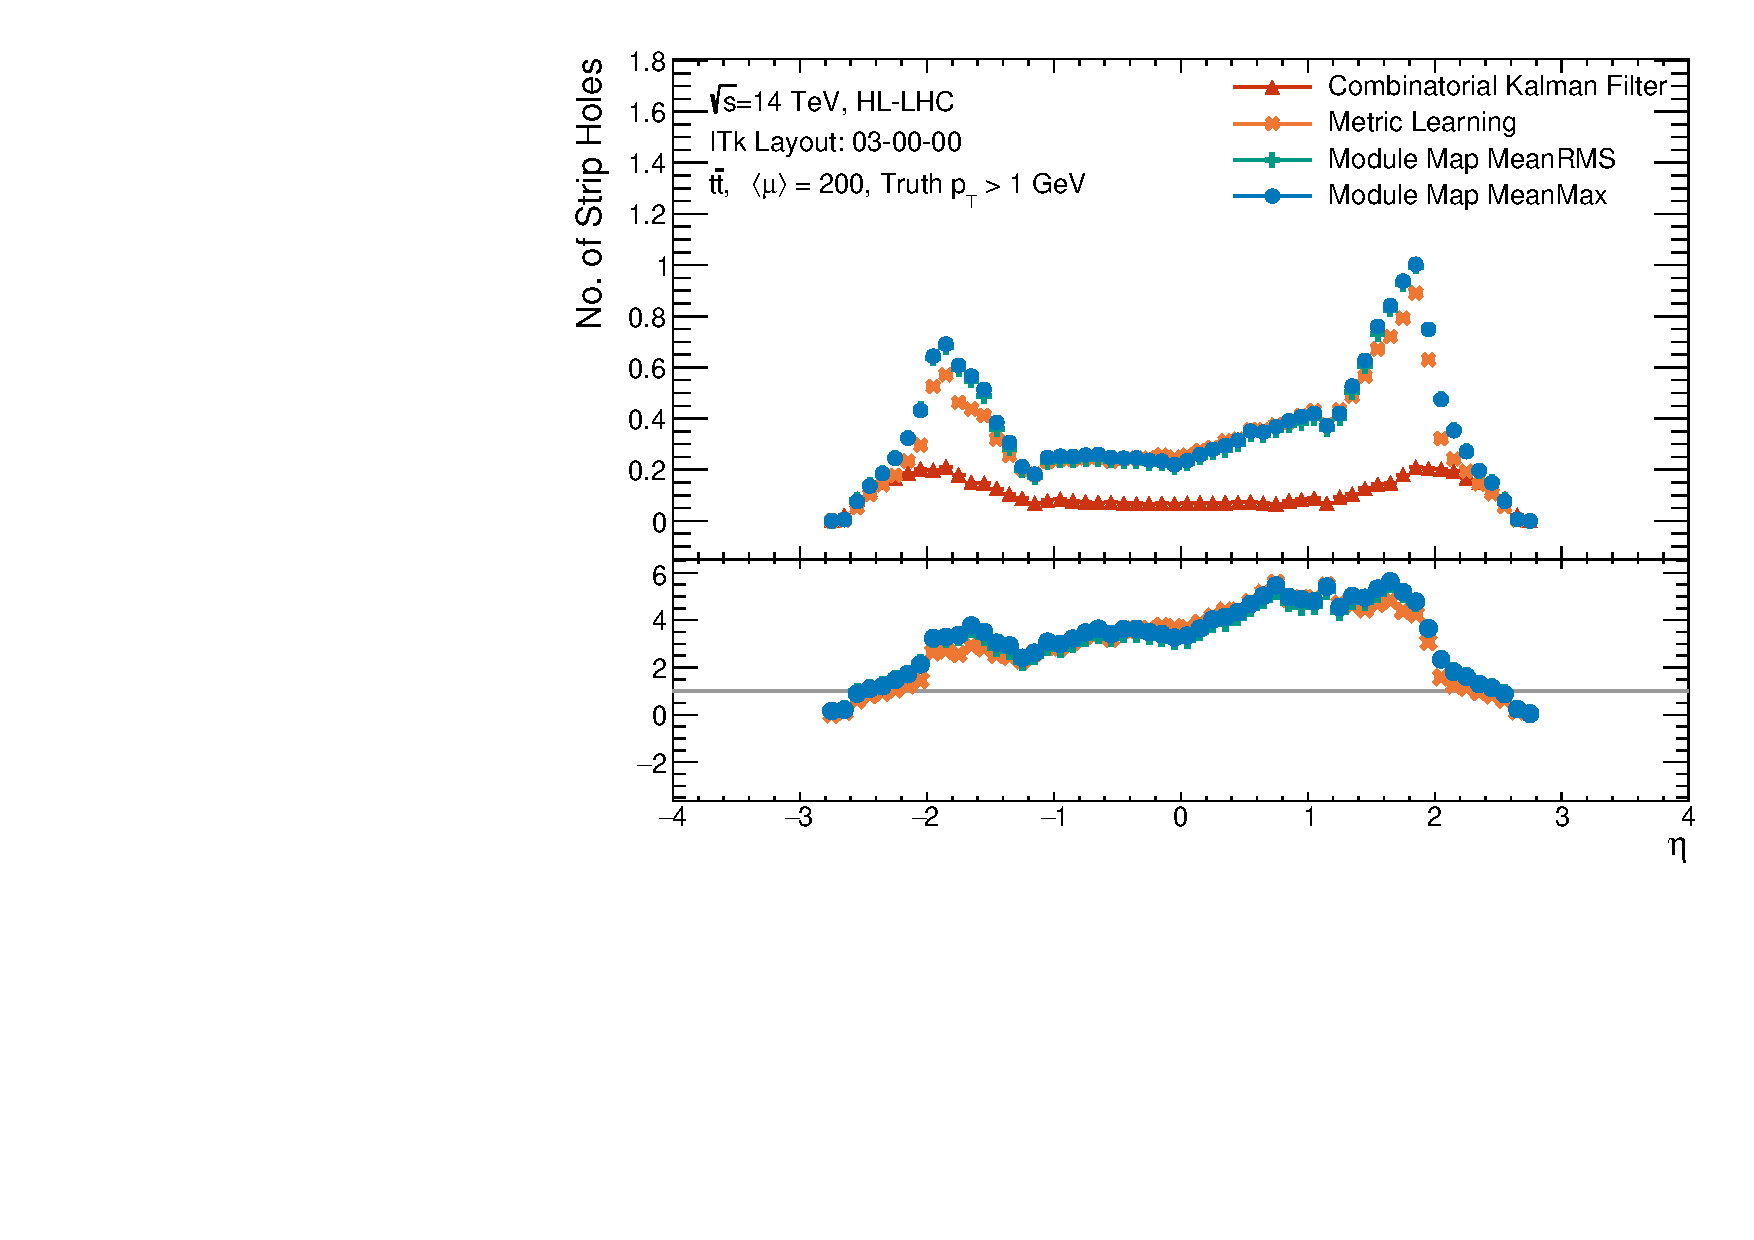
\includegraphics[width=\textwidth]{figures/ckf-gnn/HitsOnTracks/nSCTHoles_vs_eta.pdf}
    \caption{Average number of strip holes on selected track candidates}
    \label{subfig:n-strip-holes}
\end{subfigure}
    \caption{Hit content of selected track candidates, demonstrated by the average number pixel clusters (a), pixel holes (b), strip clusters (c) and strip holes (d). These quantities are shown as functions of the reconstructed pseudorapidity $\eta$.}
    \label{fig:n-hits}
\end{figure}

\newpage
In accordance with our discussion on figure \ref{subfig:res-pt-eta}, the $\eta$-independent GNN-based distributions of $\sigma(\pT)$ is manifestly wider than corresponding CKF-based distribution
The tail-heavy histograms verify that the GNN4ITk yields lower \pT resolution than does the CKF. 
Notably, the GNN-based distributions are not symmetric around $\sigma(\pT)=0$, but instead leaning more heavily toward positive values of $\sigma(\pT)$. 
Although occurring with low statistics, this asymmetry is apparent and merits further investigation.
We hypothesize that the asymmetric distribution of strip holes observed in figure \ref{subfig:n-strip-holes} could contribute to this phenomenon, but more careful inspection is needed.

% The resolution of the angles $\theta$ and $\phi$ is in good agreement with the CKF. They are shown in apprendix []
% \begin{figure}[htbp]
% \centering
% \begin{subfigure}[b]{0.65\textwidth}
%     \centering
%     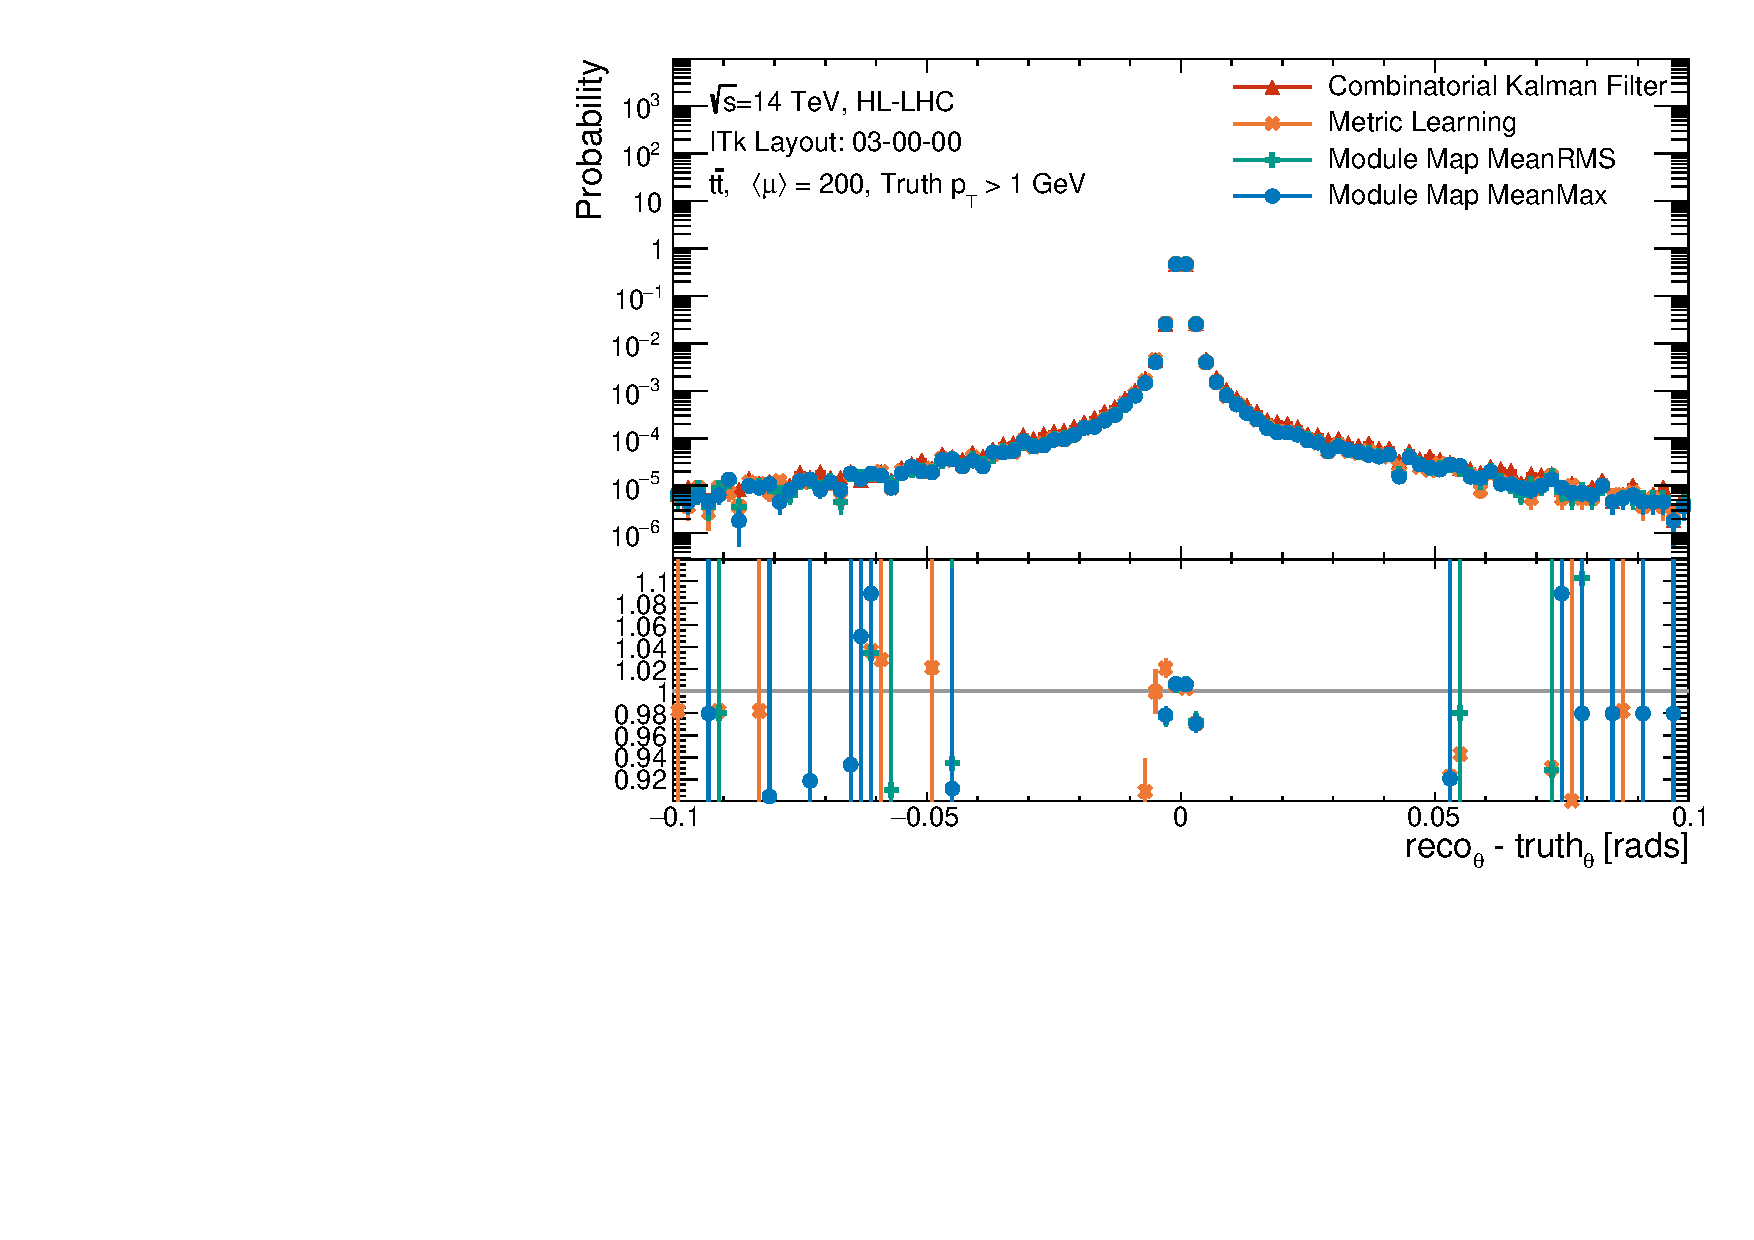
\includegraphics[width=\textwidth]{figures/ckf-gnn/Matched/Resolutions/Primary/res_theta.pdf}
%     \caption{Transverse momentum resolution $\pT  \times \left ( \frac{q}{p_{T, reco}} - \frac{q}{p_{T, truth}} \right)$}
%     \label{subfig:res-pt-hist}
% \end{subfigure}
% \begin{subfigure}[b]{0.65\textwidth}
%     \centering
%     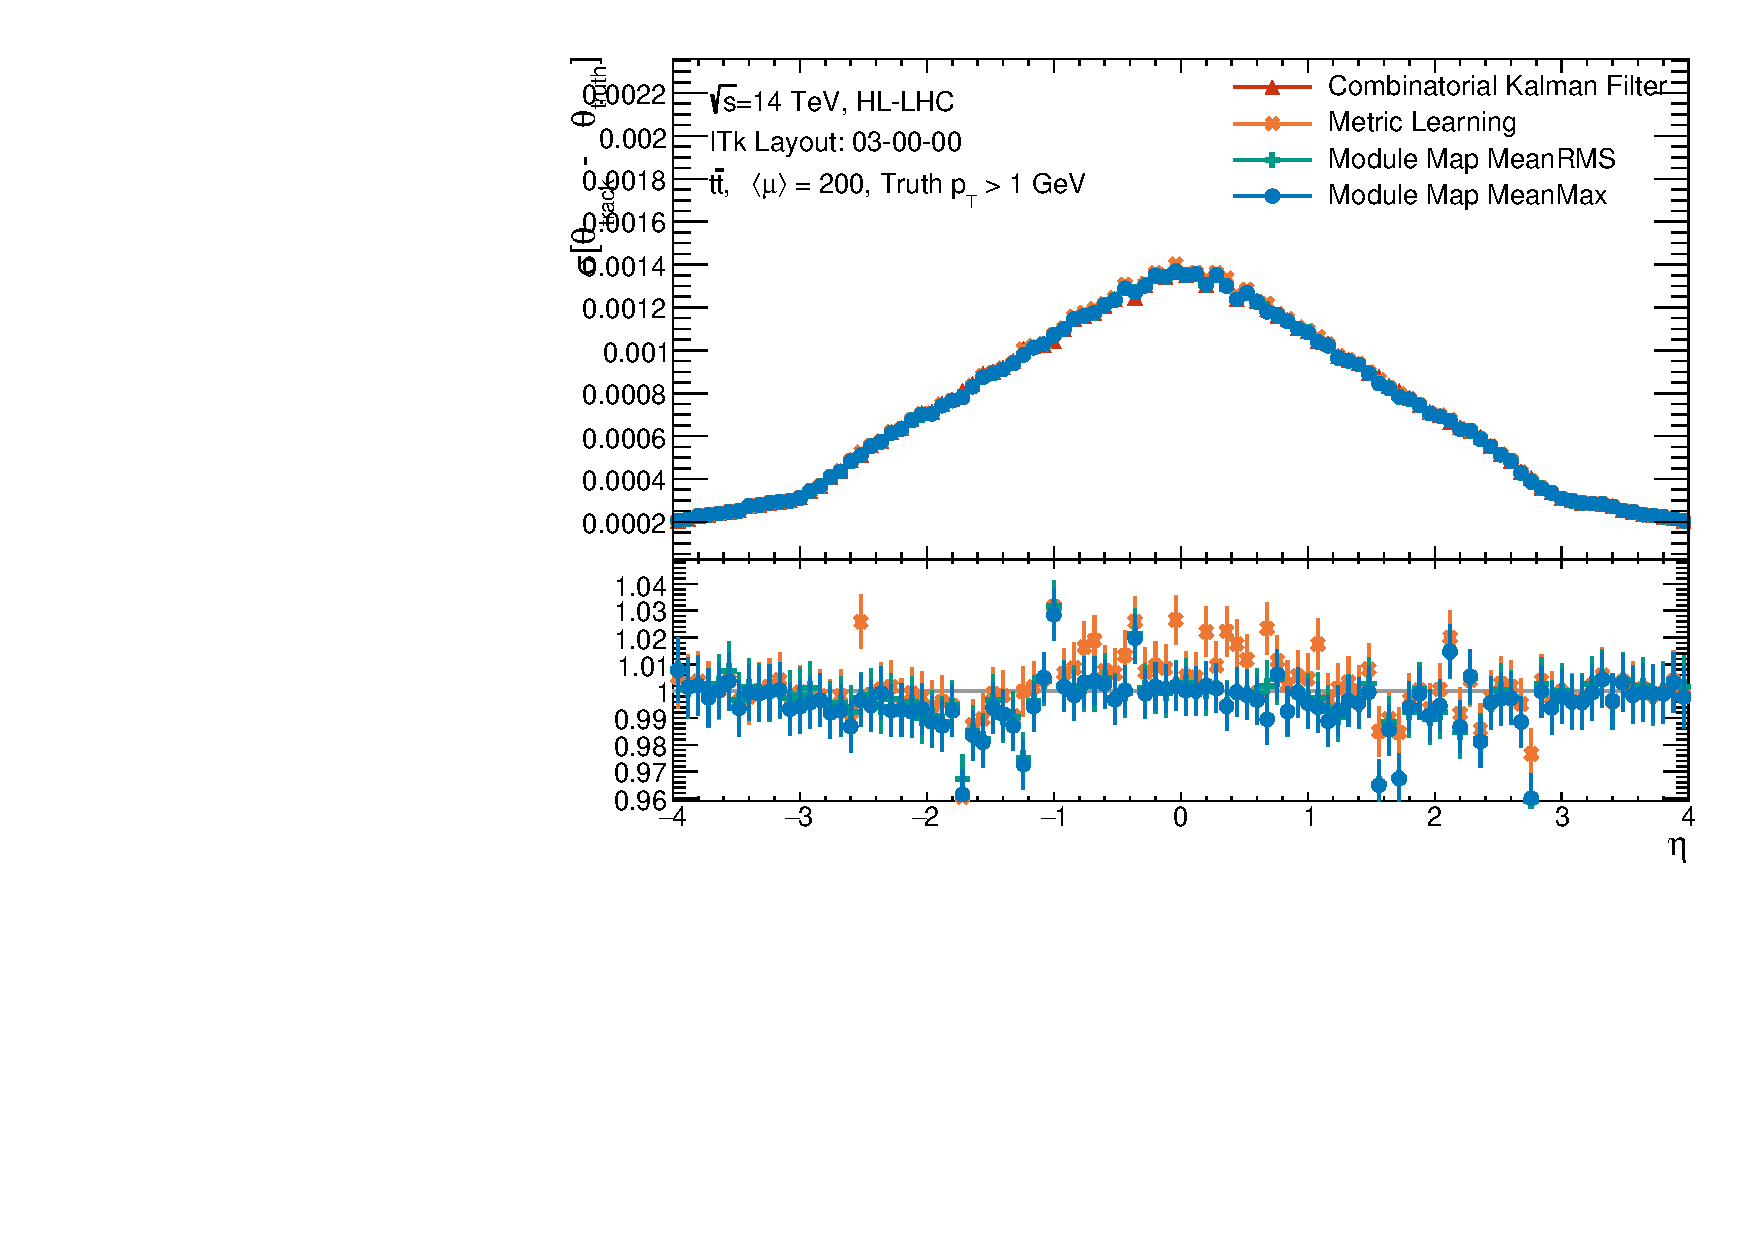
\includegraphics[width=\textwidth]{figures/ckf-gnn/Matched/Resolutions/Primary/resolution_vs_eta_theta.pdf}
%     \caption{Transverse momentum resolution $\pT \times \left ( \frac{q}{p_{T, reco}} - \frac{q}{p_{T, truth}} \right)$ as a function of $\eta$}
%     \label{subfig:res-pt-eta}
% \end{subfigure}
%     \caption{Impact parameter resolution}
%     \label{fig:res-pt}
% \end{figure}

% \begin{figure}
%     \centering
%     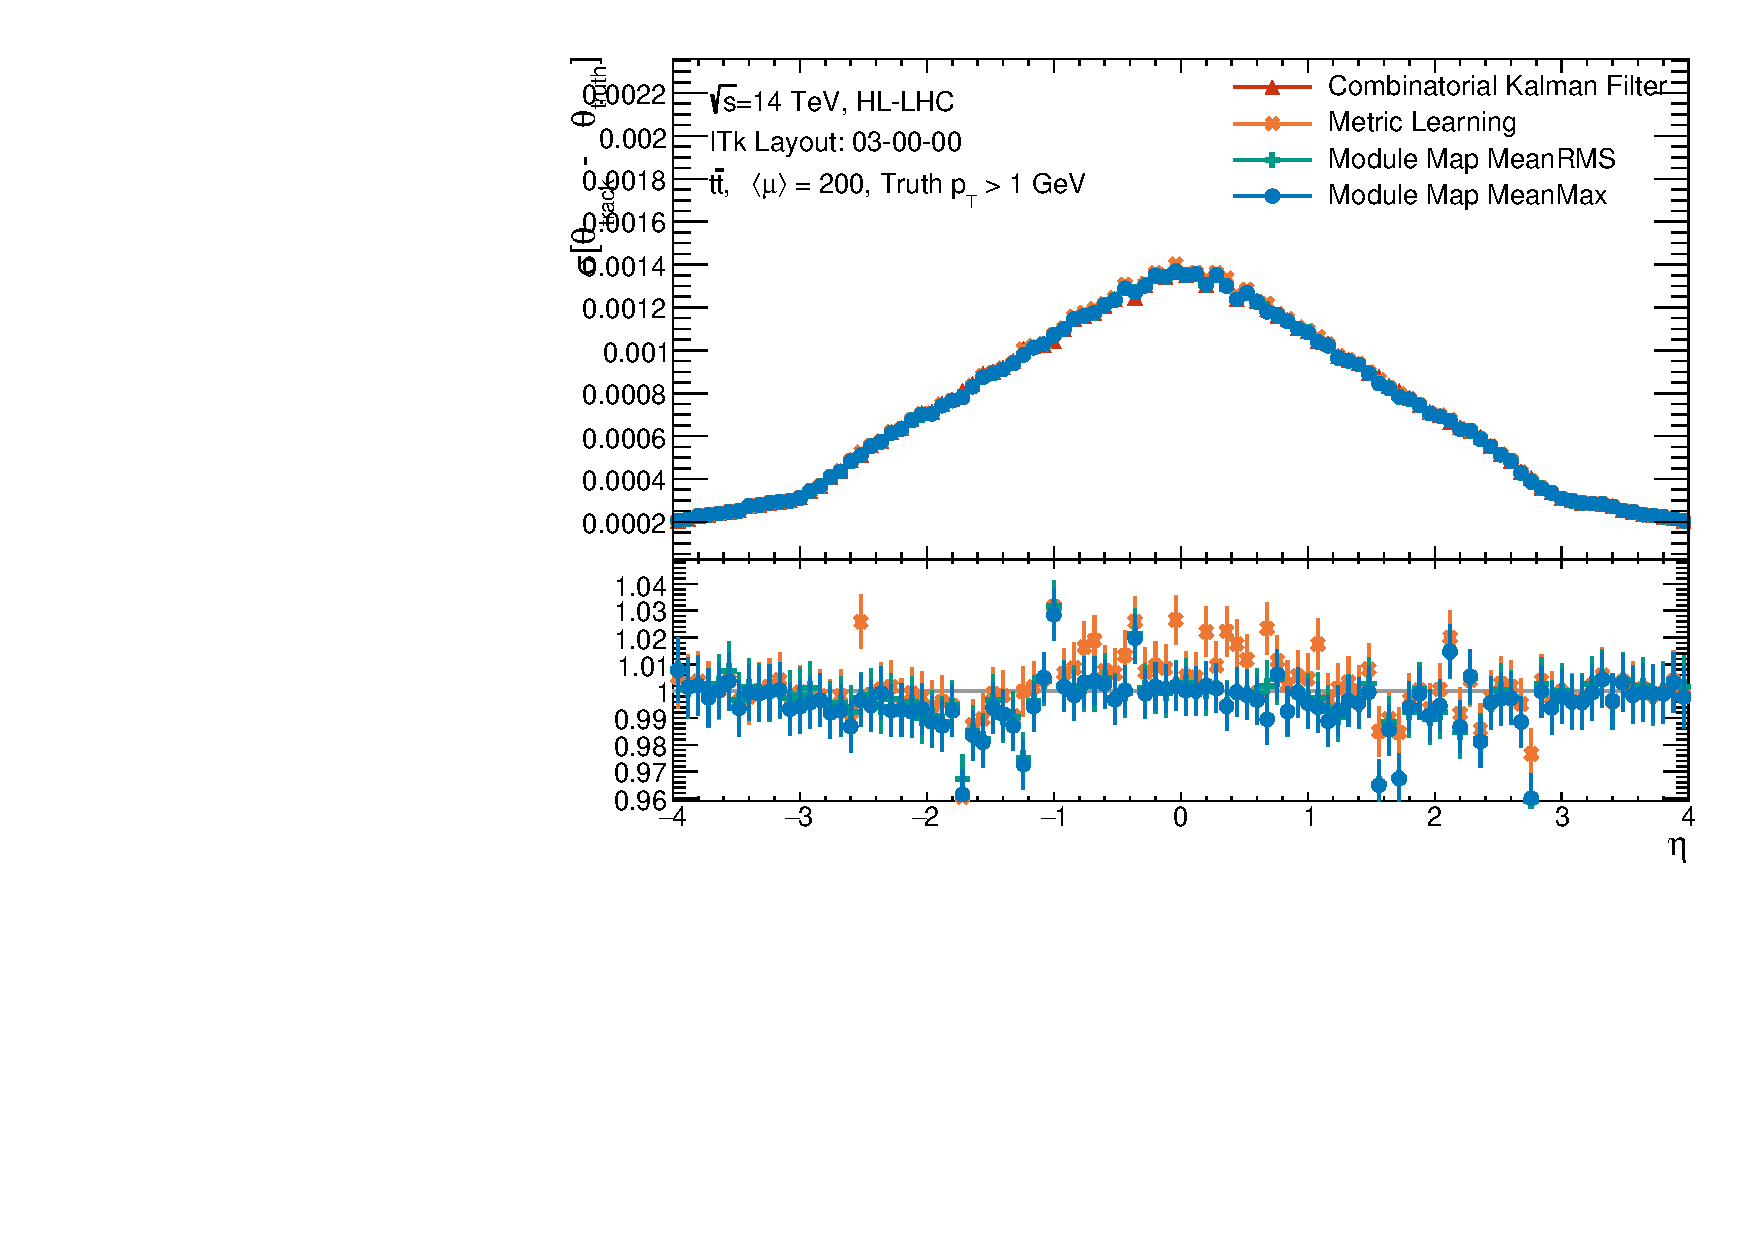
\includegraphics[width=0.65\linewidth]{figures/ckf-gnn/Matched/Resolutions/Primary/resolution_vs_eta_theta.pdf}
%     \caption{Caption}
%     \label{fig:enter-label}
% \end{figure}

% \begin{figure}
%     \centering
%     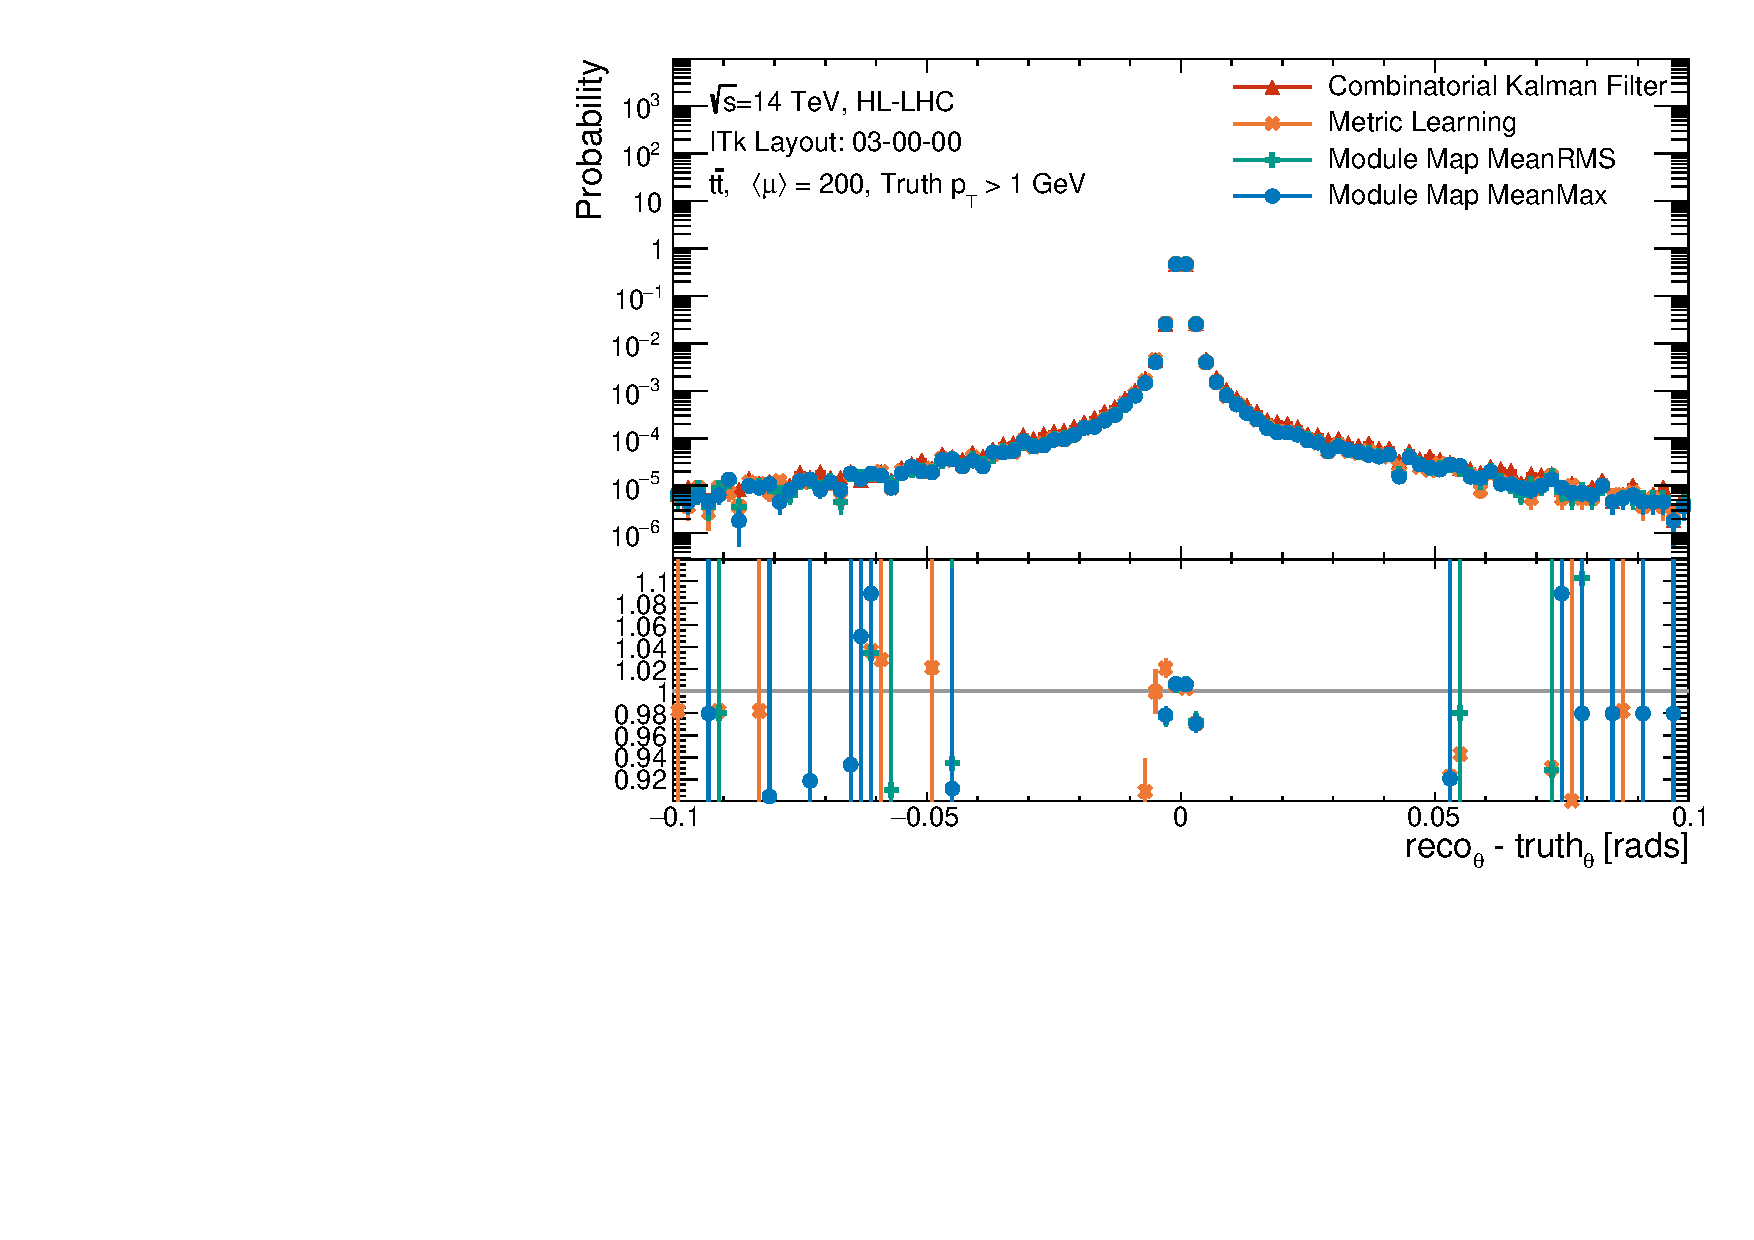
\includegraphics[width=0.75\linewidth]{figures/ckf-gnn/Matched/Resolutions/Primary/res_theta.pdf}
%     \caption{Caption}
%     \label{fig:enter-label}
% \end{figure}
